% !Mode:: "TeX:UTF-8"
% !TEX program = xelatex

%%%%%%%%%% Port for macOS %%%%%%%%%%%
% Modified: Qin Yubo

\def\usewhat{xelatex}
\documentclass[12pt,openany,twoside]{book}
%强制目录页的第一页的页眉页脚样式
\AtBeginDocument{\addtocontents{toc}{\protect\thispagestyle{only_foot}}}
                                                     % 本科生毕业论文通常采用单页排版
\input{setup/package}                                % 定义本文所使用宏包
\graphicspath{{figures/}}                            % 定义所有的图像文件在 figures 子目录下
\usepackage{makecell}
\begin{document}                                     % 开始全文
\renewcommand{\algorithmcfname}{算法}
% !Mode:: "TeX:UTF-8"
%  Authors: 张井   Jing Zhang: prayever@gmail.com     天津大学2010级管理与经济学部信息管理与信息系统专业硕士生
%           余蓝涛 Lantao Yu: lantaoyu1991@gmail.com  天津大学2008级精密仪器与光电子工程学院测控技术与仪器专业本科生

%%%%%%%%%% Fonts Definition and Basics %%%%%%%%%%%%%%%%%
\newcommand{\song}{\songti}    % 宋体
\newcommand{\fs}{\fangsong}        % 仿宋体
\newcommand{\kai}{\kaishu}      % 楷体
\newcommand{\hei}{\heiti}      % 黑体
\newcommand{\li}{\lishu}        % 隶书
\newcommand{\kaiGB}{\CJKfamily{kai}}      % 楷体GB2312, 用于独创性说明
\newcommand{\yihao}{\fontsize{26pt}{26pt}\selectfont}       % 一号, 1.倍行距
\newcommand{\xiaoyi}{\fontsize{24pt}{24pt}\selectfont}      % 小一, 1.倍行距
\newcommand{\erhao}{\fontsize{22pt}{1.25\baselineskip}\selectfont}       % 二号, 1.25倍行距
\newcommand{\xiaoer}{\fontsize{18pt}{18pt}\selectfont}      % 小二, 单倍行距
\newcommand{\sanhao}{\fontsize{16pt}{16pt}\selectfont}      % 三号, 1.倍行距
\newcommand{\xiaosan}{\fontsize{15pt}{15pt}\selectfont}     % 小三, 1.倍行距
\newcommand{\sihao}{\fontsize{14pt}{14pt}\selectfont}       % 四号, 1.0倍行距
\newcommand{\xiaosi}{\fontsize{12pt}{20pt}\selectfont}      % 小四, 1.倍行距
\newcommand{\wuhao}{\fontsize{10.5pt}{10.5pt}\selectfont}   % 五号, 单倍行距
\newcommand{\xiaowu}{\fontsize{9pt}{9pt}\selectfont}        % 小五, 单倍行距

\setmainfont{Times New Roman}

%\CJKcaption{gb_452}
%\CJKtilde  % 重新定义了波浪符~的意义
\newcommand\prechaptername{第}
\newcommand\postchaptername{章}

% 调整罗列环境的布局
\setitemize{leftmargin=3em,itemsep=0em,partopsep=0em,parsep=0em,topsep=-0em}
\setenumerate{leftmargin=3em,itemsep=0em,partopsep=0em,parsep=0em,topsep=0em}
%\setlength{\baselineskip}{20pt}
%\renewcommand{\baselinestretch}{1.38} % 设置行距

%避免宏包 hyperref 和 arydshln 不兼容带来的目录链接失效的问题。
\def\temp{\relax}
\let\temp\addcontentsline
\gdef\addcontentsline{\phantomsection\temp}

% 自定义项目列表标签及格式 \begin{publist} 列表项 \end{publist}
\newcounter{pubctr} %自定义新计数器
\newenvironment{publist}{%%%%%定义新环境
\begin{list}{[\arabic{pubctr}]} %%标签格式
    {
     \usecounter{pubctr}
     \setlength{\leftmargin}{2.5em}     % 左边界 \leftmargin =\itemindent + \labelwidth + \labelsep
     \setlength{\itemindent}{0em}     % 标号缩进量
     \setlength{\labelsep}{1em}       % 标号和列表项之间的距离,默认0.5em
     \setlength{\rightmargin}{0em}    % 右边界
     \setlength{\topsep}{0ex}         % 列表到上下文的垂直距离
     \setlength{\parsep}{0ex}         % 段落间距
     \setlength{\itemsep}{0ex}        % 标签间距
     \setlength{\listparindent}{0pt} % 段落缩进量
    }}
{\end{list}}%%%%%

\makeatletter
\renewcommand\normalsize{
  \@setfontsize\normalsize{12pt}{12pt} % 小四对应12pt
  \setlength\abovedisplayskip{4pt}
  \setlength\abovedisplayshortskip{4pt}
  \setlength\belowdisplayskip{\abovedisplayskip}
  \setlength\belowdisplayshortskip{\abovedisplayshortskip}
  \setlength{\baselineskip}{20pt} % 设置固定行间距为20pt
  \let\@listi\@listI}
\def\defaultfont{\renewcommand{\baselinestretch}{1.0}\normalsize\selectfont}
% 设置行距和段落间垂直距离
\renewcommand{\CJKglue}{\hskip -0.08pt plus 0.08\baselineskip} % 每行大概35个字符

\makeatother
%%%%%%%%%%%%% Contents %%%%%%%%%%%%%%%%% 目录样式修改,(天津大学关于博士、硕士学位论文统一格式的规定 2016.10.24)


\renewcommand{\contentsname}{目\qquad 录}
\setcounter{tocdepth}{2}
\titlecontents{chapter}[0em]{\vspace{0pt}\xiaosi\song}%
             {\prechaptername\thecontentslabel\postchaptername\quad}{} %
             {\hspace{.5em}\titlerule*[7pt]{.}\xiaosi\contentspage}
\titlecontents{section}[2em]{\vspace{0pt}\xiaosi\song} %
            {\thecontentslabel\quad}{} %
            {\hspace{.5em}\titlerule*[7pt]{.}\xiaosi\contentspage}
\titlecontents{subsection}[4em]{\vspace{0pt}\xiaosi\song} %
            {\thecontentslabel\quad}{} %
            {\hspace{.5em}\titlerule*[7pt]{.}\xiaosi\contentspage}
%\titlecontents{subsubsection}[6em]{\vspace{0pt}\xiaosi\song} %
%            {\thecontentslabel\quad}{} %
%            {\hspace{.5em}\titlerule*[7pt]{.}\xiaosi\contentspage}

%%%%%%%%%% Chapter and Section %%%%%%%%%%%%%%%%% 各级标题样式((天津大学关于博士、硕士学位论文统一格式的规定 2016.10.24))
\setcounter{secnumdepth}{4}
\setlength{\parindent}{2em}
\renewcommand{\chaptername}{\prechaptername\thechapter\postchaptername}
\titleformat{\chapter}{\centering\xiaosan\hei}{\chaptername}{1em}{}
\titlespacing{\chapter}{0pt}{33pt}{33pt}
\titleformat{\section}{\sihao\hei}{\thesection}{1em}{}
\titlespacing{\section}{0pt}{21pt}{21pt}
\titleformat{\subsection}{\sihao\hei}{\thesubsection}{1em}{}
\titlespacing{\subsection}{0pt}{13pt}{13pt}
\titleformat{\subsubsection}{\xiaosi\hei}{\thesubsubsection}{1em}{}
\titlespacing{\subsubsection}{0pt}{10pt}{10pt}

%%%%%%%%%% Table, Figure and Equation %%%%%%%%%%%%%%%%%
\renewcommand{\tablename}{表} % 插表题头
\renewcommand{\figurename}{图} % 插图题头
\renewcommand{\thefigure}{\arabic{chapter}-\arabic{figure}} % 使图编号为 7-1 的格式 %\protect{~}
\renewcommand{\thetable}{\arabic{chapter}-\arabic{table}}%使表编号为 7-1 的格式
\renewcommand{\theequation}{\arabic{chapter}-\arabic{equation}}%使公式编号为 7-1 的格式
\renewcommand{\thesubfigure}{(\alph{subfigure})}%使子图编号为 (a)的格式
\renewcommand{\thesubtable}{(\alph{subtable})} %使子表编号为 (a)的格式
\makeatletter
\renewcommand{\p@subfigure}{\thefigure~} %使子图引用为 7-1 a) 的格式,母图编号和子图编号之间用~加一个空格
\makeatother

\renewcommand{\arraystretch}{1.2}   % 扩大表格行距,以近似达到垂直居中
\setlength{\abovecaptionskip}{5pt}  % 图标标题文字与图或表之间的间隔
\setlength{\belowcaptionskip}{5pt}
%% 定制浮动图形和表格标题样式
\makeatletter
\long\def\@makecaption#1#2{%
   \vskip\abovecaptionskip
   \sbox\@tempboxa{\centering\wuhao\song{#1\qquad #2} }%
   \ifdim \wd\@tempboxa >\hsize
     \centering\wuhao\song{#1\qquad #2} \par
   \else
     \global \@minipagefalse
     \hb@xt@\hsize{\hfil\box\@tempboxa\hfil}%
   \fi
   \vskip\belowcaptionskip}
\makeatother
\captiondelim{~~~~} %用来控制longtable表头分隔符

%%%%%%%%%% Theorem Environment %%%%%%%%%%%%%%%%%
\theoremstyle{plain}
\theorembodyfont{\song\rmfamily}
\theoremheaderfont{\hei\rmfamily}
\newtheorem{theorem}{定理~}[chapter]
\newtheorem{lemma}{引理~}[chapter]
\newtheorem{axiom}{公理~}[chapter]
\newtheorem{proposition}{命题~}[chapter]
\newtheorem{corollary}{推论~}[chapter]
\newtheorem{definition}{定义~}[chapter]
\newtheorem{conjecture}{猜想~}[chapter]
\newtheorem{example}{例~}[chapter]
\newtheorem{remark}{注~}[chapter]
% \newtheorem{algorithm}{算法~}[chapter]
\newenvironment{proof}{\noindent{\hei 证明:}}{\hfill $ \square $ \vskip 4mm}
\theoremsymbol{$\square$}

%%%%%%%%%% Page: number, header and footer  %%%%%%%%%%%%%%%%%

%\frontmatter 或 \pagenumbering{roman}
%\mainmatter 或 \pagenumbering{arabic}
\makeatletter
\renewcommand\frontmatter{\clearpage
  \@mainmatterfalse
  \pagenumbering{Roman}} % 正文前罗马字体编号
\makeatother

%%%%%%%%%% References %%%%%%%%%%%%%%%%%
\renewcommand{\bibname}{参考文献}
% 重定义参考文献样式,来自thu
\makeatletter
\renewenvironment{thebibliography}[1]{%
   \chapter*{\bibname}%
   \xiaosi
   \list{\@biblabel{\@arabic\c@enumiv}}%
        {\renewcommand{\makelabel}[1]{##1\hfill}
         \setlength{\baselineskip}{17pt}
         \settowidth\labelwidth{0.5cm}
         \setlength{\labelsep}{0pt}
         \setlength{\itemindent}{0pt}
         \setlength{\leftmargin}{\labelwidth+\labelsep}
         \addtolength{\itemsep}{-0.7em}
         \usecounter{enumiv}%
         \let\p@enumiv\@empty
         \renewcommand\theenumiv{\@arabic\c@enumiv}}%
    \sloppy\frenchspacing
    \clubpenalty4000%
    \@clubpenalty \clubpenalty
    \widowpenalty4000%
    \interlinepenalty4000%
    \sfcode`\.\@m}
   {\def\@noitemerr
     {\@latex@warning{Empty `thebibliography' environment}}%
    \endlist\frenchspacing}
\makeatother

\addtolength{\bibsep}{3pt} % 增加参考文献间的垂直间距
\setlength{\bibhang}{2em} %每个条目自第二行起缩进的距离

% 参考文献引用作为上标出现
%\newcommand{\citeup}[1]{\textsuperscript{\cite{#1}}}
\makeatletter
    \def\@cite#1#2{\textsuperscript{[{#1\if@tempswa , #2\fi}]}}
\makeatother
%% 引用格式
\bibpunct{[}{]}{,}{s}{}{,}

%%%%%%%%%% Cover %%%%%%%%%%%%%%%%%
% 封面、摘要、版权、致谢格式定义
\makeatletter
\def\ctitle#1{\def\@ctitle{#1}}\def\@ctitle{}
\def\etitle#1{\def\@etitle{#1}}\def\@etitle{}
\def\caffil#1{\def\@caffil{#1}}\def\@caffil{}
\def\cmacrosubject#1{\def\@cmacrosubject{#1}}\def\@cmacrosubject{}
\def\cmacrosubjecttitle#1{\def\@cmacrosubjecttitle{#1}}\def\@cmacrosubjecttitle{}
\def\csubject#1{\def\@csubject{#1}}\def\@csubject{}
\def\csubjecttitle#1{\def\@csubjecttitle{#1}}\def\@csubjecttitle{}
\def\cgrade#1{\def\@cgrade{#1}}\def\@cgrade{}
\def\cauthor#1{\def\@cauthor{#1}}\def\@cauthor{}
\def\cauthortitle#1{\def\@cauthortitle{#1}}\def\@cauthortitle{}
\def\csupervisor#1{\def\@csupervisor{#1}}\def\@csupervisor{}
\def\csupervisortitle#1{\def\@csupervisortitle{#1}}\def\@csupervisortitle{}
\def\ccorsupervisor#1{\def\@ccorsupervisor{#1}}\def\@ccorsupervisor{}
\def\ccorsupervisortitle#1{\def\@ccorsupervisortitle{#1}}\def\@ccorsupervisortitle{}
\def\cfirstsubject#1{\def\@cfirstsubject{#1}}\def\@cfirstsubject{}   % “一级学科”
\def\cfirstsubjecttitle#1{\def\@cfirstsubjecttitle{#1}}\def\@cfirstsubjecttitle{} % 一级学科名称
\def\teachertable#1{\def\@teachertable{#1}}\def\@teachertable{}  % 答辩老师表格
\def\cdate#1{\def\@cdate{#1}}\def\@cdate{}
\def\declaretitle#1{\def\@declaretitle{#1}}\def\@declaretitle{}
\def\declarecontent#1{\def\@declarecontent{#1}}\def\@declarecontent{}
\def\authorizationtitle#1{\def\@authorizationtitle{#1}}\def\@authorizationtitle{}
\def\authorizationcontent#1{\def\@authorizationcontent{#1}}\def\@authorizationconent{}
\def\authorizationadd#1{\def\@authorizationadd{#1}}\def\@authorizationadd{}
\def\authorsigncap#1{\def\@authorsigncap{#1}}\def\@authorsigncap{}
\def\supervisorsigncap#1{\def\@supervisorsigncap{#1}}\def\@supervisorsigncap{}
\def\signdatecap#1{\def\@signdatecap{#1}}\def\@signdatecap{}
\long\def\cabstract#1{\long\def\@cabstract{#1}}\long\def\@cabstract{}
\long\def\eabstract#1{\long\def\@eabstract{#1}}\long\def\@eabstract{}
\def\ckeywords#1{\def\@ckeywords{#1}}\def\@ckeywords{}
\def\ekeywords#1{\def\@ekeywords{#1}}\def\@ekeywords{}

%在book文件类别下,\leftmark自动存录各章之章名,\rightmark记录节标题
\pagestyle{fancy}
%去掉章节标题中的数字 务必放到\pagestyle{fancy}之后才会起作用
%%不要注销这一行,否则页眉会变成:“第1章1  绪论”样式
\renewcommand{\chaptermark}[1]{\markboth{\chaptername~\ #1}{}}
  \fancyhf{}
%   \fancyhead[C]{\song\wuhao \leftmark} % 页眉显示章节名称
  \fancyhead[CO]{\song\wuhao \leftmark}  % 奇数页,显示章标题
  \fancyhead[CE]{\song\wuhao 天津大学硕士学位论文} % 偶数页,显示“天津大学硕士学位论文”
  \fancyfoot[C]{\song\xiaowu ~\thepage~}
  \renewcommand{\headrulewidth}{0.7pt}%
  \renewcommand{\footrulewidth}{0pt}%

\fancypagestyle{plain}{% 设置开章页页眉页脚风格
    \fancyhf{}%
    \fancyhead[C]{\song\wuhao \leftmark}
    \fancyfoot[C]{\song\xiaowu ~\thepage~ } %%首页页脚格式
    \renewcommand{\headrulewidth}{0.7pt}%
    \renewcommand{\footrulewidth}{0pt}%
}

\fancypagestyle{only_foot}{% 设置摘要、目录的页眉页脚风格:无页眉((天津大学关于博士、硕士学位论文统一格式的规定 2016.10.24)貌似要这种only_foot的样式)
    \fancyhf{}%
    \fancyfoot[C]{\song\xiaowu ~\thepage~ }
    \renewcommand{\headrulewidth}{0pt}%
    \renewcommand{\footrulewidth}{0pt}%
}


\newlength{\@title@width}
\def\@put@covertitle#1{\makebox[\@title@width][s]{#1}}
% 定义封面
\def\makecover{
\clearpage{\pagestyle{empty}\cleardoublepage}
   \phantomsection
    \pdfbookmark[-1]{\@ctitle}{ctitle}

    \begin{titlepage}
      \vspace*{0.8cm}
      \begin{center}

      \vspace*{1cm}
      \begin{center}
      \renewcommand{\baselinestretch}{1.25} % 设置行距
      \song\erhao\textbf{\@ctitle} % 修改成宋体加粗 (天津大学关于博士、硕士学位论文统一格式的规定, 2016.10.24)
      \renewcommand{\baselinestretch}{1.25} % 设置行距
      \end{center}
      \vspace*{1cm}

    %  \vspace*{1cm}

      \begin{center}
      \renewcommand{\baselinestretch}{1.25} % 设置行距
      \song\erhao\textbf{\@etitle}  % 修改成宋体加粗1.25倍行距(英文默认变成了Times new Roman) (天津大学关于博士、硕士学位论文统一格式的规定, 2016.10.24)
      \renewcommand{\baselinestretch}{1.25} % 设置行距
      \end{center}

      \vspace*{1cm} %3cm
      \setlength{\@title@width}{5em}
      {\song\sihao
      \begin{tabular}{p{\@title@width}@{:}l}
        \@put@covertitle{\@cfirstsubjecttitle} & \@cfirstsubject \\
        \@put@covertitle{\@csubjecttitle} & \@csubject \\
        \@put@covertitle{\@cauthortitle} & \@cauthor \\
        \@put@covertitle{\@csupervisortitle} & \@csupervisor \\
        \@put@covertitle{\@ccorsupervisortitle} & \@ccorsupervisor \\
      \end{tabular}
      }
      
      \vspace*{1cm}
      {\@teachertable}


  \vspace*{1.5cm}
  \song\sihao\@caffil \\
  \song\sihao\@cdate

\end{center}
%  另起一页: 独创性声明和学位论文版权使用授权书
\newpage
    \clearpage{\pagestyle{empty}\cleardoublepage} %去除空白页的页眉页脚(由于每章从奇数页开始因此有空白页)
    \thispagestyle{empty} %去掉页眉页脚
    \vspace*{1cm}
    \renewcommand{\baselinestretch}{1} % 设置行距
    \begin{center}\song\xiaoer{\@declaretitle}\end{center}\par
    \vspace*{0.5cm}
    \song\xiaosi{\@declarecontent}\par
    \vspace*{1cm}
    {\song\xiaosi
    \@authorsigncap \makebox[2.5cm][s]{}
    \@signdatecap \makebox[2cm][s]{} 年 \makebox[1cm][s]{} 月 \makebox[1cm][s]{} 日
    }

    \vspace*{3cm}
    \begin{center}\song\xiaoer{\@authorizationtitle}\end{center}\par
    \vspace*{1cm}
    {
    \song\xiaosi{\@authorizationcontent}

    \@authorizationadd\par
    }

    \vspace*{2cm}
    {\song\xiaosi\setlength{\parindent}{-0.45em}
    \begin{tabularx}{\textwidth}{ll}
        \@authorsigncap \makebox[3.5cm][s]{}  & \@supervisorsigncap \makebox[3.5cm][s]{}   \\
         &  \\
        \@signdatecap \makebox[1.5cm][s]{} 年 \makebox[1cm][s]{} 月 \makebox[1cm][s]{} 日 &
         \@signdatecap \makebox[1.5cm][s]{} 年 \makebox[1cm][s]{} 月 \makebox[1cm][s]{} 日 \\
    \end{tabularx}
    }
\end{titlepage}

%%%%%%%%%%%%%%%%%%%   Abstract and Keywords  %%%%%%%%%%%%%%%%%%%%%%%
\clearpage{\pagestyle{empty}\cleardoublepage} %去除空白页的页眉页脚(由于每章从奇数页开始因此有空白页)
\markboth{摘~要}{摘~要}
\addcontentsline{toc}{chapter}{摘\qquad 要}
\chapter*{\centering\song\erhao\textbf{摘\qquad 要}}
\thispagestyle{only_foot}

\setcounter{page}{1}
\song\defaultfont
\@cabstract
\vspace{\baselineskip}

%\hangafter=1\hangindent=52.3pt\noindent   %如果取消该行注释,关键词换行时将会自动缩进
\noindent
{\song\sihao\textbf{ 关键词:}} \@ckeywords

%%%%%%%%%%%%%%%%%%%   English Abstract  %%%%%%%%%%%%%%%%%%%%%%%%%%%%%%
\clearpage{\pagestyle{empty}\cleardoublepage} %去除空白页的页眉页脚(由于每章从奇数页开始因此有空白页)
\markboth{ABSTRACT}{ABSTRACT}
\addcontentsline{toc}{chapter}{ABSTRACT}
\chapter*{\centering\erhao\textbf{ABSTRACT}}
\thispagestyle{only_foot}
\@eabstract
\vspace{\baselineskip}

%\hangafter=1\hangindent=60pt\noindent  %如果取消该行注释,KEY WORDS换行时将会自动缩进
\noindent
{\sihao\textbf{KEY WORDS:}}  \@ekeywords
}

\makeatother                       % 完成对论文各个部分格式的设置
\frontmatter                               % 以下是论文导言部分,包括论文的封面,中英文摘要和中文目录
% % !Mode:: "TeX:UTF-8"

% %%  可通过增加或减少 setup/format.tex中的
% %%  第274行 \setlength{\@title@width}{8cm}中 8cm 这个参数来 控制封面中下划线的长度。

% \cheading{天津大学~2016~届本科生毕业论文}      % 设置正文的页眉,需要填上对应的毕业年份
% \ctitle{基于顾客有限理性预期的定价与供应链结构}    % 封面用论文标题,自己可手动断行
% \caffil{管理与经济学部} % 学院名称
% \csubject{工业工程}   % 专业名称
% \cgrade{2012~级}            % 年级
% \cauthor{秦昱博}            % 学生姓名
% \cnumber{3012209017}        % 学生学号
% \csupervisor{杨道箭}        % 导师姓名
% \crank{副教授}              % 导师职称

% \cdate{\the\year~年~\the\month~月~\the\day~日}

% \cabstract{
% 中文摘要一般在~400~字以内,简要介绍毕业论文的研究目的、方法、结果和结论,语言力求精炼。中英文摘要均要有关键词,一般为~3~—~7~个。字体为小四号宋体,各关键词之间要有分号。英文摘要应与中文摘要相对应,字体为小四号~Times New Roman,详见模板。
% }

% \ckeywords{关键词~1;关键词~2;关键词~3;……;关键词~7(关键词总共~3~—~7~个,最后一个关键词后面没有标点符号)}

% \eabstract{
% The upper bound of the number of Chinese characters is 400. The abstract aims at introducing the research purpose, research methods, research results, and research conclusion of graduation thesis, with refining words. Generally speaking, both the Chinese and English abstracts require the keywords, the number of which varies from 3 to 7, with a semicolon between adjacent words. The font of the English Abstract is Times New Roman, with the size of 12pt(small four).
% }

% \ekeywords{keyword 1, keyword 2, keyword 3, ……, keyword 7 (no punctuation at the end)}

% \makecover

% \clearpage


% !Mode:: "TeX:UTF-8"


\ctitle{基于生成式对抗网络的图像编辑与多模态图像转换}  %封面用论文标题,自己可手动断行
\etitle{Generative Adversarial Networks Based Image Editing and Multi Modal Image Translation}
\caffil{天津大学智能与计算学部} %学院名称
\cfirstsubjecttitle{\textbf{专业类别}}
\cfirstsubject{计算机技术}   %专业
\csubjecttitle{\textbf{研究方向}}
\csubject{计算机视觉}   %专业
\cauthortitle{\textbf{作者姓名}}     % 学位
\cauthor{刘家旭}   %学生姓名
\csupervisortitle{\textbf{指导教师}}
\csupervisor{朱鹏飞~~副教授} %导师姓名
\ccorsupervisortitle{\textbf{企业导师}}
\ccorsupervisor{刘昕} %导师姓名

\teachertable{
\begin{table}[h]
\centering
\song\xiaosi{
\begin{tabularx}{\textwidth}{|*{4}{>{\centering\arraybackslash}X|}}
\hline
\textbf{答辩日期}                & \multicolumn{3}{c|}{2021 年   月   日}       \\ \hline
\textbf{答辩委员会}               & \textbf{姓名} & \textbf{职称} & \textbf{工作单位} \\ \hline
\textbf{主席}                  &             &             &               \\ \hline
\multirow{2}{*}{\textbf{委员}} &             &             &               \\ \cline{2-4} 
                             &             &             &               \\ \hline
\end{tabularx}}
\end{table}}


\declaretitle{独创性声明}
\declarecontent{
本人声明所呈交的学位论文是本人在导师指导下进行的研究工作和取得的研究成果,除了文中特别加以标注和致谢之处外,论文中不包含其他人已经发表或撰写过的研究成果,也不包含为获得 {\underline{\kaiGB{\sihao{\textbf{~~天津大学~~}}}}} 或其他教育机构的学位或证书而使用过的材料。与我一同工作的同志对本研究所做的任何贡献均已在论文中作了明确的说明并表示了谢意。
}
\authorizationtitle{学位论文版权使用授权书}
\authorizationcontent{
本学位论文作者完全了解{\underline{\kaiGB{\sihao{\textbf{~~天津大学~~}}}}}有关保留、使用学位论文的规定。特授权{\underline{\kaiGB{\sihao{\textbf{~~天津大学~~}}}}} 可以将学位论文的全部或部分内容编入有关数据库进行检索,并采用影印、缩印或扫描等复制手段保存、汇编以供查阅和借阅。同意学校向国家有关部门或机构送交论文的复印件和磁盘。
}
\authorizationadd{(保密的学位论文在解密后适用本授权说明)}
\authorsigncap{学位论文作者签名:}
\supervisorsigncap{导师签名:}
\signdatecap{签字日期:}


\cdate{\CJKdigits{\the\year} 年\CJKnumber{\the\month} 月 \CJKnumber{\the\day} 日}
% 如需改成二零一二年四月二十五日的格式,可以直接输入,即如下所示
\cdate{二零二一年十月}
% \cdate{\the\year 年\the\month 月 \the\day 日} % 此日期显示格式为阿拉伯数字 如2012年4月25日
\cabstract{

生成式对抗网络(Generative Adversarial Nets,GANs)是2014年由Goodfellow等人提出的基于对抗训练的生成模型,伴随着深度学习的发展,GANs采用了更加高效的网络结构,同时研究人员不断提出更适合对抗训练的损失函数,GANs生成数据的质量有了很大提高,目前已广泛用于图像生成、图像编辑、图像转换、语音与音乐合成等领域。

虽然GANs在各类应用领域取得了极佳的成果,但仍存在一些不足,如:在图像属性编辑方面,隐空间编辑方法是当前的研究热点,但隐空间本身存在语义耦合的问题;在多模态图像转换方面,现有的方法难以对多个输入之间的相关性高效建模。本文梳理了GANs的发展和在图像方面的应用,并针对目前基于GANs的图像编辑与多模态图像转换存在的问题,做了如下的研究:

(1)为了解决GANs隐空间存在语义耦合的问题,并更准确地控制生成图像的属性,我们提出了属性一致生成对抗网络ACGAN。具体来说,我们预定义了正交的语义方向,从而形成正交的语义空间,并将隐变量分解为内容变量和属性变量,其中属性变量位于正交属性空间中,表示每种属性的强度。最后,我们在训练GANs的过程中约束属性变量与生成图像属性的一致性。由于语义方向是正交的,从而在理论上保证属性之间的解耦。

(2)多模态图像转换是图像转换的特例,可用于多模态图像数据补全。在本文中,我们探索了如何通过注意力机制对多个模态的相关性建模,并提出了一种联合注意力生成式对抗网络JAGAN。JAGAN包含两个重要的注意力模块:模态内注意力和模态间注意力。模态内注意力用于过滤与目标模态无关的信息,模态间注意力用于输入模态间的信息互补。二者的关系在于模态内注意力提供模态间注意力必需的特征兼容性。

本文在人脸、自然风景、医学图像等数据集上做了大量实验,通过定量和定量两方面的实验分析,验证了所提出模型相对于现有方法的先进性。

% 就基于GANs的图像编辑而言,研究表明,在预训练GANs的隐空间中进行特定的向量运算,我们可以人为控制生成图像的属性变化。受此影响,现有的基于GANs的图像编辑方法聚焦于在隐空间搜索属性对应的语义方向,然后将这些语义方向用于隐空间的向量运算,从而改变生成图像的属性。然而,这类方法往往存在语义耦合的问题,即在改变某一属性时,其他属性也发生了变化。为了解决语义耦合问题,并更准确地控制生成图像的属性,我们提出了属性一致生成对抗网络(Attribute Consistent Generative Adversarial Nets),简称ACGAN。具体来说,我们预定义了正交的语义方向形成正交的语义空间,并将隐变量分解为内容变量和属性变量,其中属性变量位于正交属性空间中,表示每种属性的强度。最后,我们在训练GANs的过程中约束属性变量与生成图像属性的一致性。由于语义方向是正交的,从而在理论上保证属性之间的解耦。

% 如今从临床诊断到公共安全,许多实际场景都需要多模态图像。在多模态图像转换方面,GANs刚刚被应用到多模态图像转换,就展现出了惊人的性能,但由于多模态数据获取难度大,数据集规模往往较小,因此难以对多个输入之间的相关性高效建模,多模态图像转换仍然非常具有挑战性。在本文中,我们探索了如何通过注意力机制对多个模态的相关性建模,并提出了一种联合注意力生成式对抗网络 (Joint Attention Generative Adversarial Networks, JAGAN) 框架。JAGAN包含两个重要的注意力模块:模态内注意力和模态间注意力,充分挖掘了多模态的跨模态一致性和模态间互补性,实验表明我们提出的JAGAN生成的多模态图像质量显著高于其他方法。
    
% JAGAN通过可用的多模态图像生成缺失的模态图像。为了更有效地提取所需模态对应的多模态表示,我们使用自表示网络来驱动注意力模块。提取出的多模态特征可以与目标模态保持通道级的一致性,极大地提高了多模态图像转换性能。

}

\ckeywords{生成式对抗网络,图像编辑,多模态图像转换,语义耦合}

\eabstract{

Generative Adversarial Nets (GANs) is a generative model based on adversarial training proposed by Goodfellow et al. in 2014. With the development of deep learning, GANs adopt a more efficient network structure, and researchers continue to propose more suitable loss functions for adversarial training. The quality of the data generated by GANs is significantly improved. GANs have been widely used in image generation, image editing, image translation, voice and music synthesis, and other fields.

Although GAN has achieved inadequate results in various application fields, there are still some concerns. First, the latent space editing methods suffer from semantic entanglements.  Although GANs based image translation achieved great progress, multimodal image translation is still challenging due to the difficulty in modeling correlations between multiple inputs. Here, we discuss the development and application of GANs and do the following research to solve existing problems of GANs-based image editing and multimodal image translation.

(1) To solve the problem of semantic entanglements in latent space and control attributes of generated images more accurately, we propose Attribute Consistent Generative Adversarial Nets, termed ACGAN. We pre-defined orthogonal semantic directions, forming the orthogonal attribute space. We decompose the latent code into the content code and the attribute code. The consistency between input attribute code and attribute of generated images is optimized in the training phase. The attribute code lies in the above orthogonal space, to theoretically ensure disentanglement between attributes.

(2) Multimodal image translation is a special case of image translation, which can be used for multimodal image completion. In this article, we explored how to model the correlation of model modalities by attention mechanism, and proposed a joint attention GAN, JAGAN. JAGAN contains two important attention modules: intra-modal attention and inter-modal attention. Intra-modal attention is used to filter information that has nothing to do with the target modality, and inter-modal attention is used to complement the information between input modalities. The relationship between the two is that intra-modal attention provides the necessary feature compatibility for inter-modal attention.

In this paper, we conducted extensive experiments on datasets such as human faces, natural scenery, and medical images. Through quantitative and quantitative experimental analysis, we have verified the advanced performance of the proposed models compared to existing methods.
    

% Generative Adversarial Networks (GAN) are currently widely used in image editing, image translation and other fields.

% Recent research suggests that Generative Adversarial Networks can produce realistic images with different attributes. To precisely control each attribute of generated images, current methods search the semantic directions in the latent space of a pretrained model. Since the generative models are trained without the supervision of attribute labels, these methods yield semantic entanglement. To tackle these concerns, we propose Attribute Consistent Generative Adversarial Nets, termed ACGAN, to train an attribute-based generative model while projecting the controllable semantic directions to an orthogonal space. Specifically, we first design an attribute quantification method to obtain the continuous labels. An attribute regressor trained by them is applied to constrain the attribute consistency between the input attribute code and the generated results. We decompose the latent code into the content code and the attribute code. The attribute code lies in an orthogonal space, so as to theoretically ensure disentanglement between attributes.

% Multimodal images are required in many practical scenarios, ranging from clinical diagnosis to public security. Data missing often leads to decision bias. Although GAN based image translation achieved great progress, multimodal image translation is still challenging due to the difficulty in modeling correlations between multiple inputs. In this paper, we novelly proposed a joint attention GAN (JAGAN) framework to generate the missing modality image through available multimodal images. JAGAN contains two important attention modules: intra-modal attention and inter-modal attention, which fully explores the cross-modal consistency and inter-modal complementarity of multimodal inputs. Experiments show that quality of images generated by our proposed JAGAN is significantly higher than other methods.
% To effectively extract the multimodal representation specific to desired modality, we use a self-representation network to drive a inter-modal attention module. The extracted multimodal features can maintain kernel-level consistency with the target modality, which greatly improved the image translation performance.

}

\ekeywords{Generative Adversarial Networks, Image Editing, Multimodal Image Translation, Semantic Entanglement}

\makecover
\clearpage                      % 封面

%%%%%%%%%%   目录   %%%%%%%%%%
\clearpage{\pagestyle{empty}\cleardoublepage}
\defaultfont
\clearpage{
    \pagestyle{only_foot}
    \tableofcontents                           % 中文目录
    \thispagestyle{only_foot}
}
\clearpage{\pagestyle{empty}\cleardoublepage}

%%%%%%%%%% 正文部分内容  %%%%%%%%%%
\mainmatter\defaultfont\sloppy\raggedbottom
\chapter{绪论}

\section{生成式对抗网络的前世今生}

生成式对抗网络(Generative Adversarial Networks, GANs)自2014年由Goodfellow等人提出以来~\cite{GANs},一直是深度学习领域的热门研究方向。仅在2018年,就出现了大约11800与GANs相关的论文。换句话说,每天约有32篇,不到一个小时就有一篇相关论文问世\cite{review}。本节我将按时间顺序,以GANs领域中若干个重要工作为节点,从GANs的萌芽、发展与最新进展三个阶段,阐述GANs的发展历程及其应用。

\subsection{萌芽:机器学习领域十年来最有趣的思想}
机器学习模型分为判别式模型和生成式模型,Goodfellow等人提出的GANs正是一种生成式模型。相比于之前的生成式模型,GANs最大的贡献在于提出了一种基于对抗的训练方式。GANs由两个网络组成,分别是生成器和判别器。其中生成器将输入映射到目标空间,从而捕捉目标空间的数据分布;判别器一般是一个二值分类器,用于区分判断生成器生成的图片和数据集中真实的图片。GANs训练过程是一个交替优化生成器和判别器的过程,在这个过程中,生成器的目标是生成可以骗过判别器的图片,判别器的目标则是尽可能区分生成图片与真实图片。详细的训练过程将在第二章介绍。

原始GANs的输入是高斯噪声,这也就意味着你无法控制生成图像的类别,在这种情况下,如果需要生成猫和狗两类图片,只能在猫图片数据集和狗图片数据集上分别训练GANs。为了解决这个问题,Mehdi Mirza等人提出了条件生成式对抗网络(Conditional GANs, CGANs)~\cite{CGANs}。同时,我们也将最初的这类输入不含标签的GANs称为非条件生成式对抗网络(unconditional GANs)。如图\ref{CGAN-result}所示,CGAN可以控制生成器生成指定的手写数字。

\begin{figure}
    \centering
    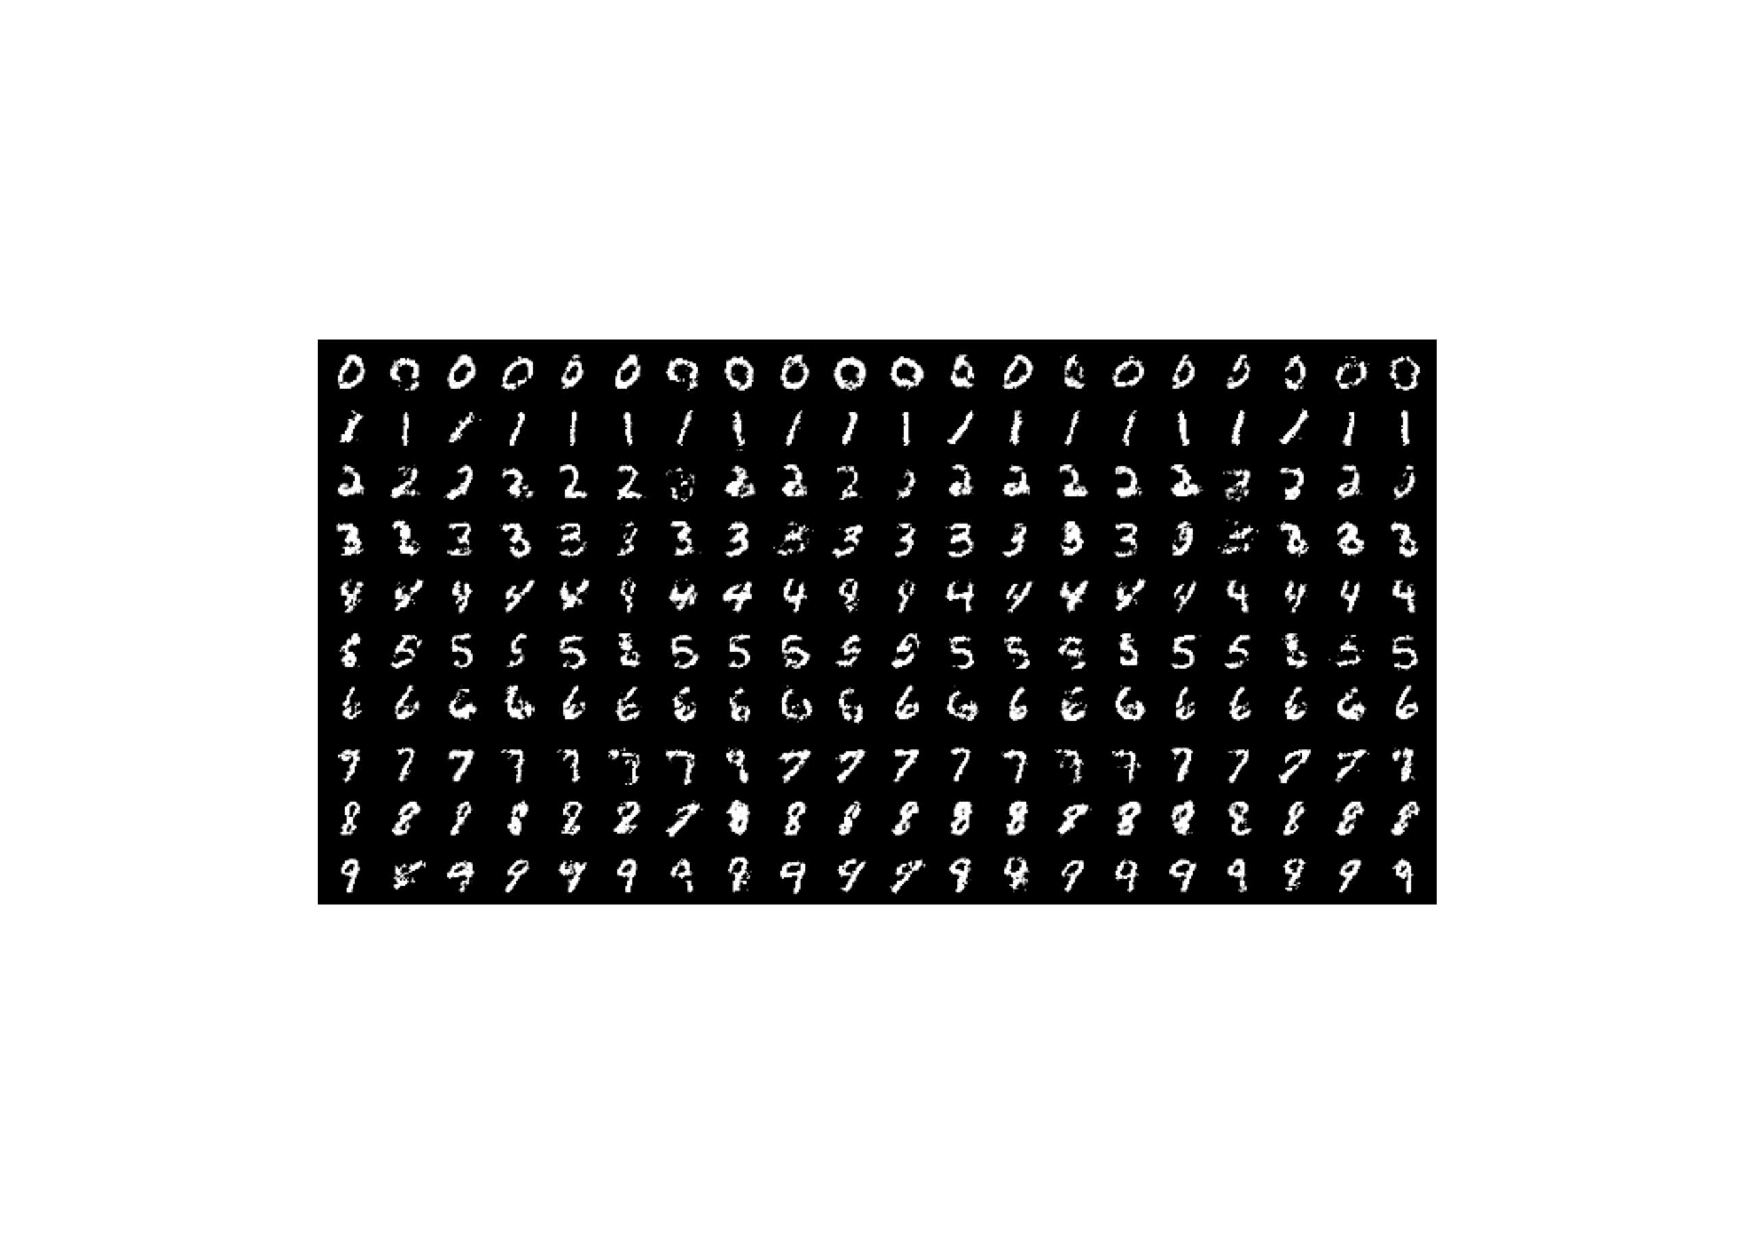
\includegraphics[width=\textwidth]{figures/CGAN-result.pdf}
    \caption{CGAN可以生成指定手写数字的类别。从上至下,CGAN生成了0-9总共10中类别的手写数字。}
    \label{CGAN-result}
\end{figure}

无论是GANs还是CGANs,此时仍受图像生成质量不高导致的实用价值不高的困扰。随着深度学习的发展,Alec Radford等人在2016年提出了使用卷积神经网络替换GANs中的多层感知机,大大提升了生成图像的质量。由于GANs已经广泛作为生成式对抗网络的概念使用,下文将称这Goodfellow等人提出的GANs模型为原始GANs。如图~\ref{GAN-DCGAN}所示,原始GANs生成的人像、自然图像质量都较差;而DCGAN能够生成较高质量的卧室图片。

\begin{figure}
    \centering
    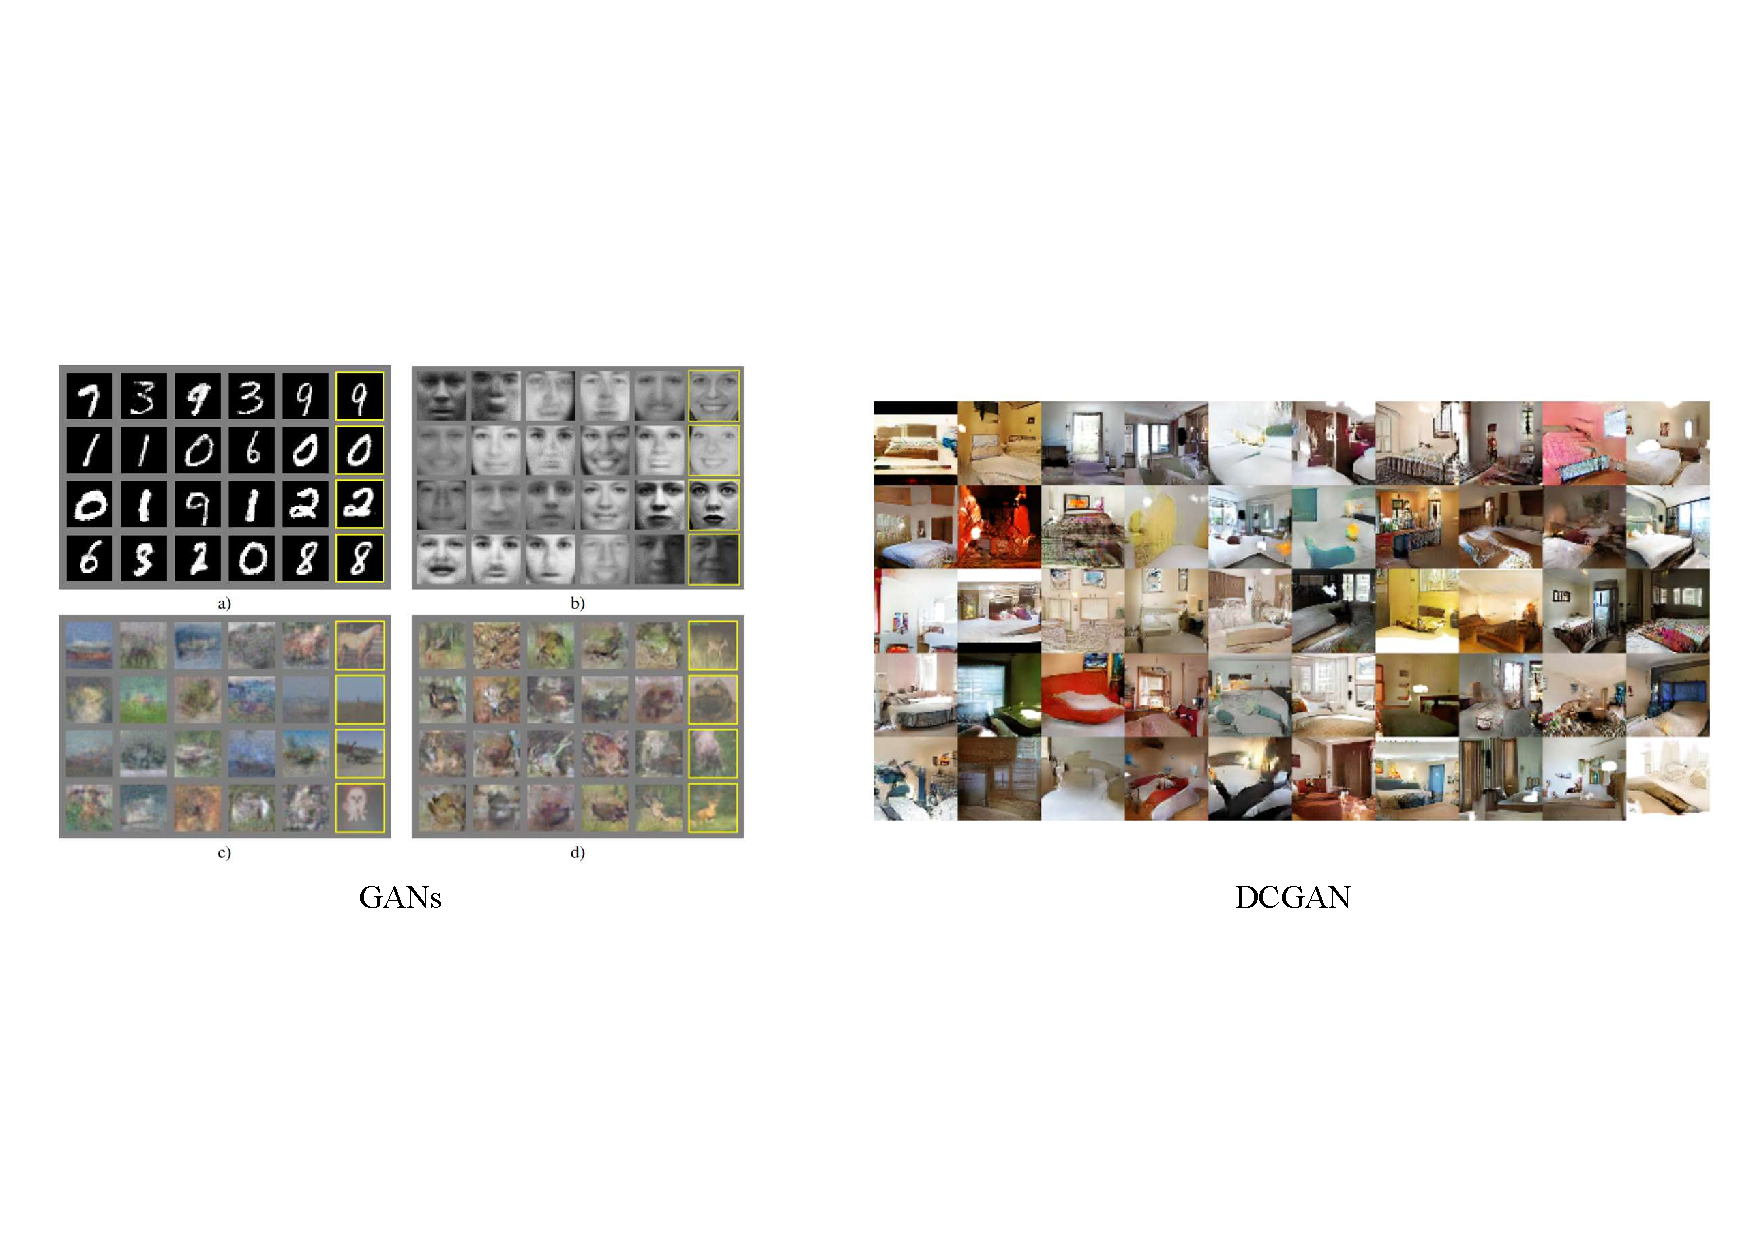
\includegraphics[width=\textwidth]{figures/GAN-DCGAN.pdf}
    \caption{GANs和DCGAN的生成效果对比}
    \label{GAN-DCGAN}
\end{figure}

至此,生成式对抗网络完成了它的萌芽阶段,其框架已经确定,最近的GANs模型基本都在这一框架内:

\begin{itemize}
\item GANs由生成器和判别器两个网络组成。
\item 训练采用对抗训练的方式。判别器致力于区分生成图像与真实图像,生成器目标是生成可以“骗过”判别器的图像。
\item 按照输入是否包含标签,GANs分为unconditional GANs和conditional GANs。
\item 就图像生成而言,生成器和判别器一般由卷积神经网络实现。
\end{itemize}

\subsection{发展:迈向以假乱真的真实图像和实际应用}
由于高分辨率图像包含更多细节,判别器更容易将生成的图像与真实图像区分开来,因此在高分辨率下训练GANs是一件很困难的事。除此之外,由于显存的限制,我们在高分辨率是只能使用较小的batch size,这进一步损害了训练时的稳定性。Odena等人在2017年提出PGGAN(Progressive Growing OF GANS)~\cite{PGGAN},作者认为可以从更简单的低分辨率图像开始逐步增加生成器和鉴别器,并随着训练的进行添加引入更高分辨率细节的新层。这种渐进式的训练方式大大加快了训练速度并提高了高分辨率下的稳定性。

时间来到2019年,BigGANs~\cite{BigGANs}探索了CGANs如何通过训练更大的模型提高生成图像的质量,StyleGAN~\cite{StyleGAN}则展示了GANs如何生成风格各异的图像。BigGANs和StyleGAN的生成结果分别如图~\ref{BigGAN}和图~\ref{StyleGAN}所示,可以看到无论是GANs(StyleGAN)还是CGANs(BigGANs),生成的图像都达到了“以假乱真”的程度。

\begin{figure}
    \centering
    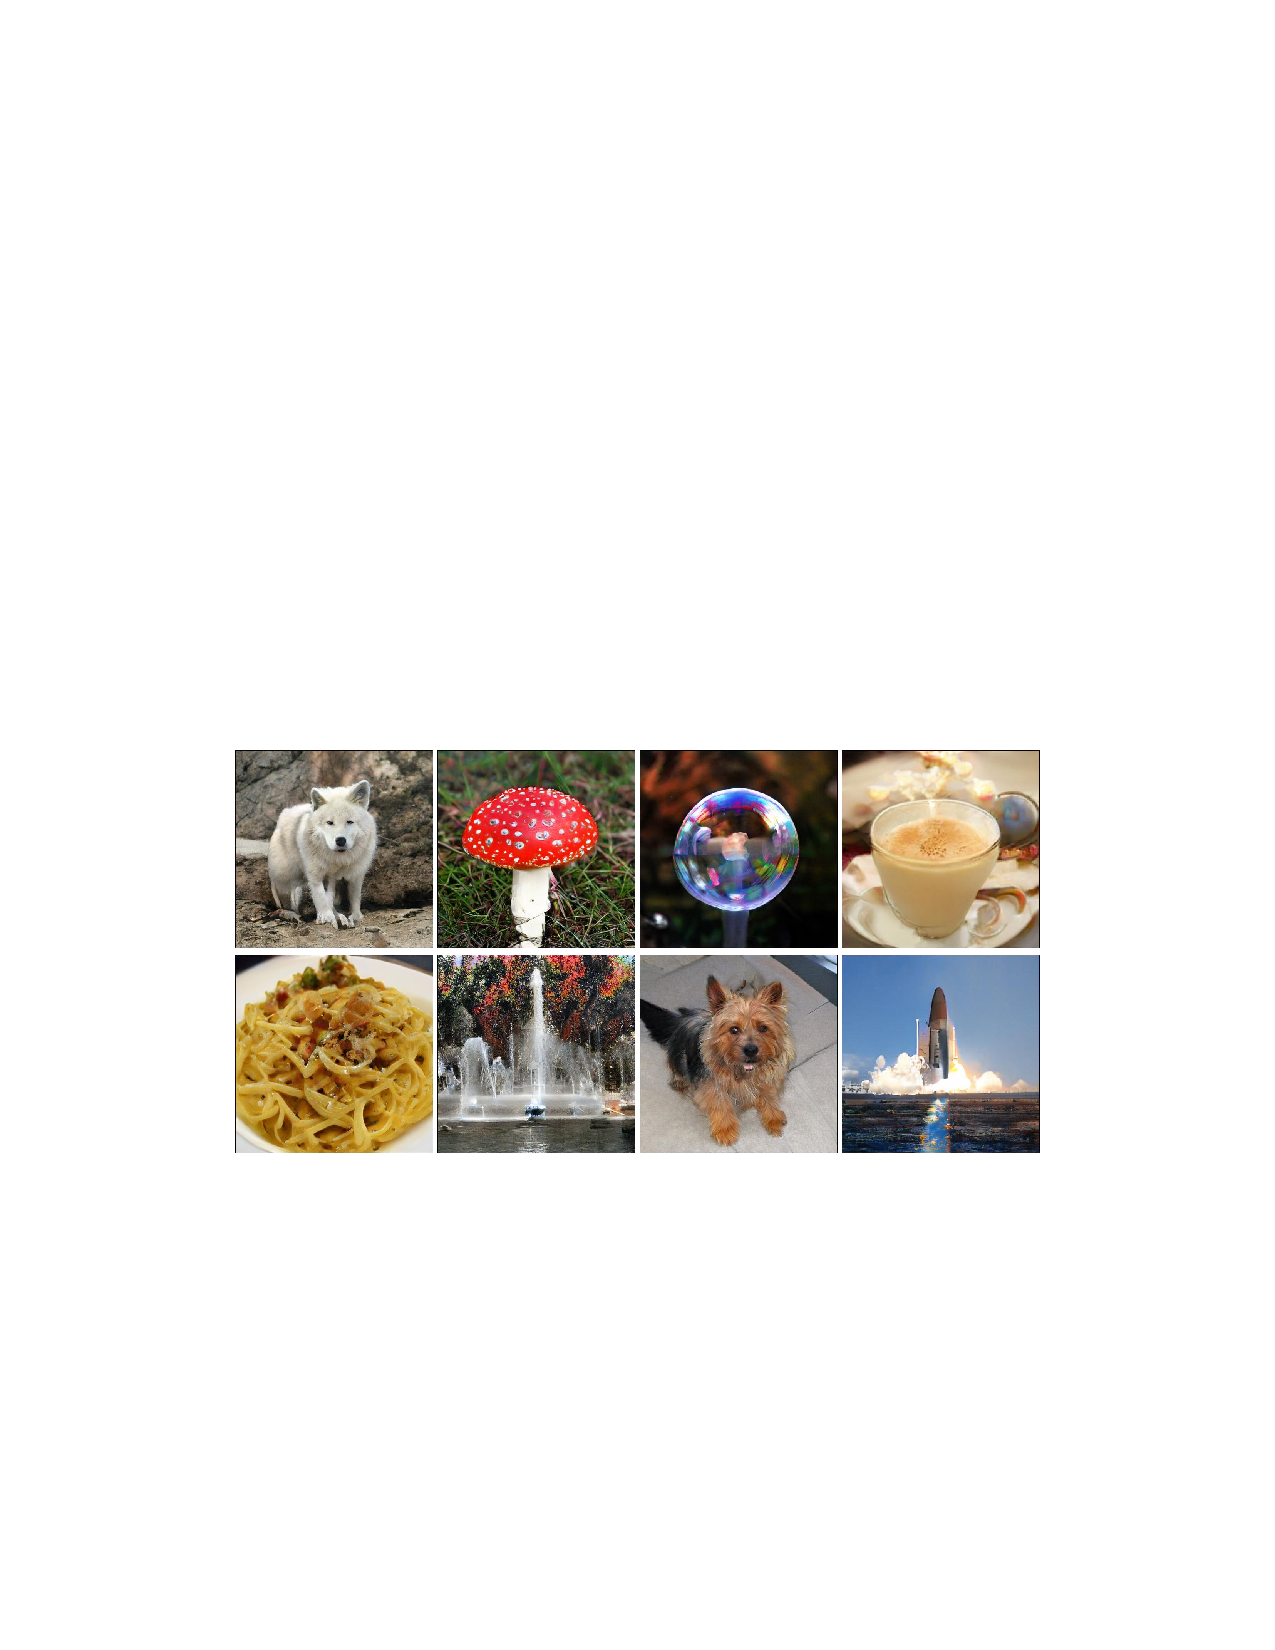
\includegraphics[width=\textwidth]{figures/BigGAN.pdf}
    \caption{BigGANs的512x512分辨率下的生成图像,可以看到生成的图像种类丰富且非常真实,但放大后仍可看出些许涂抹感。}
    \label{BigGAN}
\end{figure}

\begin{figure}
    \centering
    \includegraphics[width=\textwidth]{figures/StyleGAN.pdf}
    \caption{StyleGAN的生成结果。最上面一行与最左边一列是StyleGAN生成的不同风格的人像,中间则是两种风格混合后生成的人像。作者将这种风格混合生成人像的功能称为style mixing。}
    \label{StyleGAN}
\end{figure}


\subsection{最近进展和应用}

正如我们在上一节提到的,我们已经能够使用GANs生成足够真实且风格迥异的图片,因此研究热点逐渐转为GANs的应用。我们在这里主要介绍两类应用,一是基于GANs的属性编辑,二是基于GANs的图像转换。

CGANs的出现,使我们能够控制生成图像的类别,但我们仍无法控制生成图像的属性。例如,我们可以使用CGANs生成年轻人和老年人两类图像,但无法具体控制人物年轻或年老的程度。实际上早在DCGAN中,作者就发现了隐空间(生成器输入又称为隐变量,输入所在的空间又称为隐空间)中的向量运算可以控制生成图像的属性。受此启发,近些年出现了非常多通过在隐空间搜索语义方向的方式实现生成图像属性编辑的工作\cite{icml2020, harkonen2020ganspace, iclr2021, interfacegan, steer,variation},在这里我们将这类通过隐空间中向量预算改变生成图像属性的方法统称为隐空间编辑(latent-space editing)。

GANs很早就被用于图片转换(image translation),即将原域的图片转换为目标域的图片,经典的模型有Pix2Pix~\cite{pix2pix}、CycleGAN~\cite{cyclegan}等。本质上,这类用于图片转换的GANs是一种特殊的CGANs,此时原域的图片作为标签输入生成器。最近,研究人员提出CollaGAN~\cite{collagan}和Auto-GAN~\cite{AutoGAN},开始将GANs应用于多模态图像转换,一定程度上解决了多模态图像缺失的问题。


\section{问题和挑战}

据我们所知,现有的隐空间编辑均是:1.在预训练的GANs上搜索隐空间中属性对应的语义方向;2.在对应的语义方向上对隐变量进行向量运算。这类方法在做属性编辑时存在语义耦合的问题,即在改变某一属性时,其他属性也发生了变化。

在多模态图像变换方面,现有的基于GANs的方法没有充分利用模态间的一致性与互补性,这导致生成的目标模态图像出现信息损失。多模态数据广泛存在临床诊断等领域,缺失的信息可能会影响医生的决策。

\section{本文的贡献}

本文全面分析了GANs在属性编辑和多模态图像转换上遇到的问题和挑战,提供相应的解决方法:

(1)为了解决隐空间属性编辑语义耦合的问题,我们提出属性一致性网络。将输入隐变量分解为内容变量和属性变量,其中属性变量位于预定义的正交属性空间中,从而在理论上保证了属性编辑时的语义解耦。

(2)针对现有的基于GANs的多模态图像变换方法没有充分利用模态间的一致性与互补性的问题,我们提出联合注意力机制,在模型训练期间充分挖掘模态间的一致性与互补性,显著提高了多模态图像转换的质量与准确性。

\section{本文组织结构}

本文主要关注GANs在属性编辑和多模态图像转换上遇到的问题和挑战,提供相应的解决方案,并通过大量实验进行了验证,具体组织结构如下:

第一章简要梳理了生成对抗网络的发展历史,并引出了本文所关注的两个任务:属性编辑和多模态图像转换。最后总结了本文的创新点和贡献;

第二章全面介绍了生成对抗网络的原理与应用,特别是其在属性编辑和多模态图像上存在的不足;

第三章介绍了如何通过属性一致约束,实现天然能够控制属性连续变化的生成式对抗网络,从而解决隐空间属性编辑中的低效与耦合问题;

第四章介绍了如果使用注意力机制充分挖掘模态间的一致性与互补性,从而提高基于生成式对抗网络的多模态图像变换的质量;

第六章对全文进行总结,重点是本文的贡献和不足,为日后生成式对抗网络的研究提供了参考方向。
\clearpage{\pagestyle{empty}\cleardoublepage} % 去除空白页的页眉页脚(每章从奇数页开始,因此有空白页)
\chapter{相关概念及研究工作介绍}

\section{生成式对抗网络的理论}

\subsection{生成式对抗网络的概述}

基于生成式对抗网络~\cite{GANs}的生成模型极大的提升了图片生成的真实度。生成式对抗网络由生成器和判别器组成,生成器负责将隐变量(一般是从高斯分布采样的噪声)映射为生成的图像,判别器是一个二分类器,用于区分生成图像与真实图像。生成器和判别器以一种对抗的方式交替训练,这也是生成式对抗网络最核心的贡献。

受益于GANs广阔的应用前景,近来大量生成对抗网络相关的工作如雨后春笋般涌出,其中不乏一些重要的、对GANs理论和应用有深远影响的工作。原始GANs使用多层感知机(MLP)来实现,后来随着深度学习的发展,尤其是卷积神经网络在图像处理方面的广泛使用,Alec Radford等人在2016年提出了使用卷积神经网络替换GANs中的多层感知机~\cite{DCGAN},大大提升了生成图像的质量。在原始GANs中,生成器的输入是高斯噪声,这也就意味着你无法控制生成图像的类别。为了解决这个问题,Mehdi Mirza等人提出了条件生成式对抗网络(conditional GANs, cGANs)~\cite{CGANs},通过在输入中添加类别标签和在训练中添加分类损失,得到了能够指定生成数据类别的生成器。GANs自提出以来一直饱受训练不稳定问题的影响,Tim Salimans等人在Improved GANs~\cite{salimans2016improved}中总结了一系列训练技巧,目前已称为训练GANs的常规方案。还有一些文献~\cite{wgan, lsgan}则提出了新的损失函数,目的是更好地衡量生成数据与真实数据(训练集)分布的差距,从而提高GANs训练的稳定性。

目前GANs已经能够生成足够真实的图像,但仍需要很长的训练时间,以StyleGAN为例,在单Tesla V100显卡上训练需要接近70天!Bingchen Liu等人在2021年推出了一种轻量级GANs~\cite{lwgan},得益于其高效的网络结构和数据增广策略,只需要几个小时就能在单卡上完成训练。生成效果如图~\ref{fig:LWGAN}所示,可以看到这种轻量级GANs在生成质量上不如BigGANs、StyleGAN等重量级网络,但考虑到个人和科研机构往往计算资源有限,因此这类轻量级GANs仍有非常重要的现实意义。

\begin{figure}
    \centering
    \includegraphics[width=\textwidth]{figures/LWGAN.pdf}
    \caption{轻量级GANs在1024x1024分辨率下的生成效果}
    \label{fig:LWGAN}
\end{figure}

\subsection{损失函数}

我们用$\mathcal{L}_{GAN}(G, D)$表示GANs训练的损失函数。$\mathcal{L}_{GAN}(G, D)$的实现方式涉及到GANs训练的稳定性和生成数据的真实度,因此一直是GANs研究的重点问题。

在原始GANs中,$\mathcal{L}_{GAN}(G, D)$的计算如公式~\ref{eq:js_divergence}所示:

\begin{equation}
    \mathcal{L}_{GAN}(G, D) = E_{x \sim p_{\text {data }}(x)}[\log D(x)]+E_{z \sim p_{z}(z)}[\log (1-D(G(z)))]
    \label{eq:js_divergence}
\end{equation}

该公式本质上是生成数据与真实数据之间的JS散度。公式~\ref{eq:js_divergence}中的目标函数对训练生成器来说存在梯度消失的问题~\cite{review},解决这一问题一般的思路是重新设计目标函数。LSGAN~\cite{lsgan, lsgan2}提出使用最小二乘损失替代JS散度,WGAN~\cite{wgan}提出使用Wasserstein距离度量两个分布间的距离,Hinge损失的基本思想是让正例和负例之间的距离尽量大,最初用于支持向量机(SVM)的优化,后被迁移到GANs的训练~\cite{hinge1,hinge2,hinge3}。

\subsection{生成式对抗网络的训练}

生成器和判别器以一种对抗的方式交替训练,我们以先优化判别器为例,介绍GANs的训练流程。

在每次模型迭代中,我们先以公式~\ref{step_D}优化判别器,注意此时我们固定生成器的权重不变。

\begin{equation}
    \max _{D} V(D, G, R) = \mathcal{L}_{GAN}(G, D)
    \label{step_D}
\end{equation}

然后,我们以公式~\ref{step_G}优化生成器,同样的,此时我们固定判别器的权重不变。

\begin{equation}
    \min _{G} V(D, G, R) = \mathcal{L}_{GAN}(G, D)
    \label{step_G}
\end{equation}

将公式~\ref{step_D}和~\ref{step_G}结合起来,我们就得到了如公式~\ref{overall}所示的GANs总损失。

\begin{equation}
    \min _{G} \max _{D} V(D, G, R) = \mathcal{L}_{GAN}(G, D)
\end{equation}

重复上述步骤,直到生成器生成的图像对人来说足够真实,生成图像的真实度也可以用FID~\cite{fid}等评价指标辅助判断。与其他机器学习模型不同,生成器和判别器的损失并不能直接表明模型的好坏,需要我们通过观察生成图像的质量来判断训练进度。

\subsection{生成图像的评价指标}

我们在这里重点介绍4种生成图像的评价指标,分别是SSIM、FSIM、IS和FID,这些评价指标从不同的角度评估了生成图像的真实性,需要根据具体的任务来选择何时的评价指标。

SSIM(Structural Similarity Index Measure,结构相似性)~\cite{ssim},是一种衡量两张图片结构相似性的指标,最初用于比较无失真图像和压缩后失真影像的相似性,可看作失真影像质量的评价指标,现也用于比较任意两张图像的结构相似性。计算公式如下所示:

\begin{equation}
    \operatorname{SSIM}(x, y)=\frac{\left(2 \mu_{x} \mu_{y}+c_{1}\right)\left(2 \sigma_{x y}+c_{2}\right)}{\left(\mu_{x}^{2}+\mu_{y}^{2}+c_{1}\right)\left(\sigma_{x}^{2}+\sigma_{y}^{2}+c_{2}\right)}
\end{equation}
在这里$x$,$y$表示用于比较的两张图片,$\mu_{x}$是$x$的平均值,$\mu_{y}$为$y$的平均值,$\sigma_{x}^{2}$为的$x$方差,$\sigma_{y}^{2}$为$y$的方差,$\sigma_{x y}$为$x$,$y$的协方差。$c_{1}$与$c_{2}$均为常数,用来维持数值稳定。

FSIM(Feature Similarity Index Measure,特征相似性)~\cite{fsim},概念与SSIM类似,考察两张图像特征的相似性。

IS(Inception Score)~\cite{salimans2016improved}对每张生成图像,使用Inception模型~\cite{inception}计算条件标签分布$p(y|x)$。如果生成图像中包含有意义的物体,那么计算条件标签分布$p(y|x)$的值应该较低。另一方面,我们希望生成图像尽可能多样化,反映在边缘概率$\int p(y \mid x=G(z)) dz$上应该是较大的值。结合上述两点,IS的计算公式为:

\begin{equation}
    IS\left(p(y \mid x), p(y)\right)=\exp \left(E_{x} K L(p(y \mid x) \| p(y))\right)
\end{equation}

更高的IS分数意味着生成器能够生成具有明确语义且多样化的图像。然而,IS分数也有其劣势,如果生成模型陷入模式坍塌,IS分数可能仍然较低。

FID(Fréchet Inception Distance)~\cite{fid}是专为GANs设计的评价指标,计算方式是使用Inception模型的卷积层特征计算函数$\phi$,对真实数据分布$p_{data}$和生成数据分布$p_{g}$建模为高斯随机变量$\phi (p_{data})$和$\phi (p_{g})$,其均值为$\mu_{r}$, $\mu_{g}$,方差为$C_{r}$, $C_{g}$,最后计算:
\begin{equation}
    F I D\left(p_{\text {data }}, p_{g}\right)=\left\|\mu_{r}-\mu_{g}\right\| + tr\left(C_{r}+C_{g}-2\left(C_{r} C_{g}\right)^{1 / 2}\right)
\end{equation}
即可得到FID分数,本质上是这两个高斯分布之间的弗雷歇距离(Fréchet distance)。

\section{生成式对抗网络的应用}

\subsection{图像转换}

图像转换(Image translation)指将输入图像从原风格转换为目标风格(风格转换)或从原图像域转换为目标图像域。 随着深度学习的发展,神经网络风格迁移(neural sytle transfer)~\cite{transfer0,transfer1,transfer2}已经成为风格迁移的主流方法。 风格迁移侧重于不同的艺术风格间的转换,而图像转换~\cite{i2i0,i2i1,i2i2,cyclegan} 解决了更一般的图像域转换问题。

不同的图像转换方法侧重于从不同的角度,解决不同类型的图像转换问题。Pix2Pix~\cite{pix2pix}解决了配对图像(像素对齐的两张图像)的图像转换问题。对于损失函数,Pix2Pix的作者认为可以依靠L1损失约束低频信息,判别器仅用来鉴别高频信息是否真实,作者进一步提出了PatchGAN。 PatchGAN的核心思想是,既然判别器只用于鉴别高频信息,那么就不需要将整张图片输入到判别器中,只在patch(正方形像素块,作者最终采用了70x70的像素块作为patch)的规模上计算高频结构损失。因为不同的patch之间可以认为是相互独立的。PatchGAN对一张图片切割成不同的N x N大小的patch,判别器对每一个patch做真假判别,将一张图片所有patch的结果取平均作为最终的判别器输出。作者认为这会鼓励GANs生成的图像包含清晰的高频细节。

现实世界中更一般的实际上是非配对图像的转换,因为配对图像在大部分真实场景非常难以获取,比如我们要做马和斑马之间的转换,几乎不可能找到像素点对齐的马和斑马的配对图像。
CycleGAN~\cite{cyclegan}提出了循环一致性损失解决了非配对图像的转换问题。与常规的GANs不同,CycleGAN包含两个生成器$G_A$和$G_B$,与两个判别器$D_A$和$D_B$。假设我们有两张分别来自于$A$图像域和$B$图像域的图片$I^A$和$I^B$,非配对图像转换的难点在于,如果我们要将$I^A$转换到$B$域,我们没有$I^A$在$B$域的对应图像,因此无法用类似L1损失的方式约束像素之间的差异。在计算循环一致性损失时,先用$G_A$将$I^A$转换到$B$域,再用$G_B$将上一步的结果转换回$A$域,得到$I^A_{cyc}$,此时就可以计算$I^A$和$I^A_{cyc}$之间的差异,$I^B$和$I^B_{cyc}$的计算类似,如公式~\ref{eq:cyc}所示。

\begin{equation}
    \mathcal{L}_{\mathrm{cyc}}(G, F) =\mathbb{E}_{x \sim p_{\text {data }}(x)}\left[\|F(G(x))-x\|_{1}\right] +\mathbb{E}_{y \sim p_{\text {data }}(y)}\left[\|G(F(y))-y\|_{1}\right]
    \label{eq:cyc}
\end{equation}

无论是Pix2Pix还是CycleGAN,都是解决了两个图像域之间的转换,如果需要多个域之间互相转换,只能训练多个模型,StarGAN~\cite{stargan}通过在输入增加目标域对应的掩码(mask)和类别损失,使用单一模型解决了多个域之间互相转换的问题。

图像转换方法从整体来看,都是输入一张图像,然后转换为另一张图像,与下面要介绍的隐空间编辑方法有很大不同,因此一部分文献~\cite{iclr2021}将图像转换又称为图像空间编辑。目前大多数基于GANs的图像空间编辑方法的问题在于难以同时编辑多个属性,并精确控制生成图像中的属性强度。

\subsection{隐空间编辑}

在GANs发展的早期,Alec Radford等人就在\cite{DCGAN}中发现GANs的隐空间中通常包含有语义意义的向量算法,例如,隐空间中存在能为人脸添加微笑或眼镜的方向。我们称这类通过隐空间向量运算实现图像编辑发方法为隐空间编辑方法,区别与上文提到的图像空间编辑方法,后者是对图像直接的转换。

由于隐空间编辑使图像编辑更加简单,因此近些年来这类方法收到越来越到的关注。从隐空间编辑的监督方式来看,隐空间编辑方法分为有监督、无监督、自监督或半监督的方法。

\begin{enumerate}
\item 有监督的隐空间编辑方法采用明确的人工监督来识别隐空间中的可解释方向,如Yujun Shen等人~\cite{interfacegan}使用在CelebA数据集~\cite{celeba}上预训练的二分类器来预测人脸属性。然后使用该分类器为生成的图像及对应的隐变量生成伪标签。基于这些伪标签,可以在隐空间空间中构建分类超平面,该超平面的法线即为相应属性变化的方向。

\item 无监督通过学习一组语义上区别较大的方向~\cite{icml2020} 或基于主成分分析(PCA)的方法~\cite{harkonen2020ganspace}识别潜在的的语义方向。这些方法可能会找到有意义的方向,但其结果是不可预测的,并且需要人工解释,这导致了非监督的隐空间编辑方法难以指定所需的语义方向。

\item 自监督方法~\cite{steer,variation} 通过使用简单的几何变换(例如旋转和缩放)增加数据来搜索可解释的方向,这限制了这些方法搜索复杂属性的能力。半监督方法~\cite{nie2020semi} 调查了有限监督的影响,这很难同时精准解耦并编辑多个属性。
\end{enumerate}

以上方法的本质均是在预训练的GANs的隐空间中搜索语义方向,不可避免地受到预训练GANs的影响,由于GANs在训练时没有受到语义属性的约束,其隐空间必然存在语义耦合现象。这导致现有的隐空间编辑的方法在改变某一属性时,通常会导致其他的属性也发生变化。    

\subsection{多模态图像转换}

在图像处理、计算机视觉和计算机图形学的许多应用中,越来越依赖于多模态医学图像。例如精准医学,脑部核磁共振中存在T1、T1Gd、T2和T2-FLAIR四种模态~\cite{drevelegas2011imaging}。医生希望结合完整的多模态医学图像来做出更精确的诊断,但受限于实际条件限制(例如,受限的医疗条件、扫描时间不足以及成本/支出/资源等限制),实践中可能存在成像系统存在误差,甚至部分模态的缺失的现象~\cite{tanenbaum2017synthetic}。这些不可用的图像可能会导致医生决策出现偏差。

Dongwook Lee等人提出的CollaGAN~\cite{collagan}是第一篇将GANs用于多模态图像。与CycleGAN,Pix2Pix等单模态图像转换方法只能输入一种模态的图像不同,CollaGAN针对多模态图像转换提出了多重循环一致损失(Multiple cycle consistency loss),通过一个GANs模型解决了多模态间模态转换的问题。

CollaGAN和Auto-GAN均使用单个模型在一定程度上解决了多模态图像转换的问题,但都没有在训练过程中对模态间的一致性和互补性进行约束。

\section{本章小结}

在本章节我们总结了生成式对抗网络,图片空间编辑、隐空间编辑和多模态图像转换的原理、应用和进展,重点梳理了隐空间编辑和多模态图像现有方法的优势与不足,为后续本文解决方案的提出奠定了基础。

%\clearpage{\pagestyle{empty}\cleardoublepage}
\chapter{基于生成式对抗网络的图像编辑}

\section{引言}

生成式对抗网络~\cite{GANs}以一种对抗的方式训练生成器和鉴别器,从而对目标数据分布建模。当模型收敛时,生成器将从隐空间采样的隐变量映射到图像空间。最新的深度生成模型在生成逼真的图像方面取得了巨大进步,这些图像甚至与现实世界的照片无法区分。然而,GANs模型本身无法编辑生成图像的语义属性,比如操纵人像的年龄或场景图片的天气。

图像编辑可用于图像增强、动画设计等专业领域。目前基于GANs的图像编辑方法可以分为两类:图像空间编辑方法和隐空间编辑方法。图像空间编辑方法~\cite{cyclegan,i2i0,i2i1,i2i2} 将一张图像从源域直接转换到目标域。这些方法必须学习大量的冗余模型,因为每两个域之间的转换需要一个模型。这对于多属性编辑任务来说是灾难性的。
隐空间编辑方法侧重于在预训练的GANs的隐空间中搜索与语义相关的方向。这类方法按照监督信息可以进一步分为:无监督方法~\cite{icml2020,harkonen2020ganspace}、自监督方法~\cite{steer,variation} 和监督方法~\cite{interfacegan,iclr2021}。这类方法在做属性编辑时存在语义耦合的问题,改变一种属性通常伴随着其他属性的改变。语义耦合的根本原因在于,隐空间编辑方法所使用的预训练GANs在训练时没有受到属性的约束,其隐空间天然存在语义耦合。

为了从根本上解决这个问题,我们提出了一种输入属性与生成图像属性一致的生成式对抗网络,简称为属性一致的生成式对抗网络(Attribute Consistent Generative Adversarial Networks, ACGAN),用于图像属性编辑。
与现有方法不同,我们将隐空间分解为内容空间和属性空间:输入的隐变量由分别从内容空间(服从高斯分布)和属性空间(服从均匀分布)中采样的内容变量和属性变量组成。由于隐空间编辑方法发现的语义方向是耦合的,因此我们提出将属性空间投影到正交空间,以便将每个语义方向与其他方向分开。为了将可控语义方向投影到正交属性空间,我们进一步提出了一种属性一致损失,约束了生成图像的预测属性与输入属性变量之间的连续一致性。
然而,据我们所知,目前只有一个数据集Transient Attribute Database~\cite{scenedataset} 包含连续的属性标签,而大多数图像属性数据集~\cite{celeba,place,sun} 只包含二值标签。为了将我们的方法扩展到所有属性数据集,我们进一步提出了一种属性量化策略,将二值属性标签量化为连续值。

我们提出的属性一致性生成式对抗网络具有以下创新点:

(1)预定义了正交的语义方向,从而形成正交的语义空间,为解决隐空间编辑语义耦合问题提供了理论上的保障。

(2)提出属性一致性损失,引入属性回归器监督输入属性与生成图像属性之间的一致性。

(3)为了将我们的方法应用于更常见的二值属性数据集,我们设计了一种属性量化策略来获得连续属性伪标签,可以灵活地与现有方法集成以提高属性编辑性能。

(4)统一了GANs生成图像与属性控制两个任务,使生成器天然具有控制生成图像属性的能力,并提出了属性编辑成功率、属性增益等属性编辑评价指标。

\section{属性一致性的生成式对抗网络}

\subsection{概述}
由于隐空间本身存在语义耦合现象,因此目前大多数隐空间编辑方法都存在语义耦合的问题,即在改变生成图像的某一属性时,其他属性也发生了变化。为了从根本上解决属性耦合的问题,我们将生成器的隐变量分解为内容变量和属性变量,并将属性方向投影到正交空间中。具体来说,我们提出了一种通过正交属性一致性进行图像编辑的属性一致生成式对抗网络(ACGAN),如图~\ref{fig:framework}所示。 在图~\ref{fig:framework}(a)中,方向搜索方法~\cite{icml2020, iclr2021}找到的方向是通过比较原始图像和编辑图像的属性差异来完成的,搜索到的方向互相耦合。图~\ref{fig:framework}(b)中我们的方法使用输入属性值和生成图像的预测属性之间的属性一致损失来训练生成器。 我们预定义的方向是正交的,以便将每个语义方向与其他方向分开。
这从根本上解决了隐空间编辑中的属性耦合问题,使同时编辑多种属性成为可能。

\begin{figure}
    \centering
    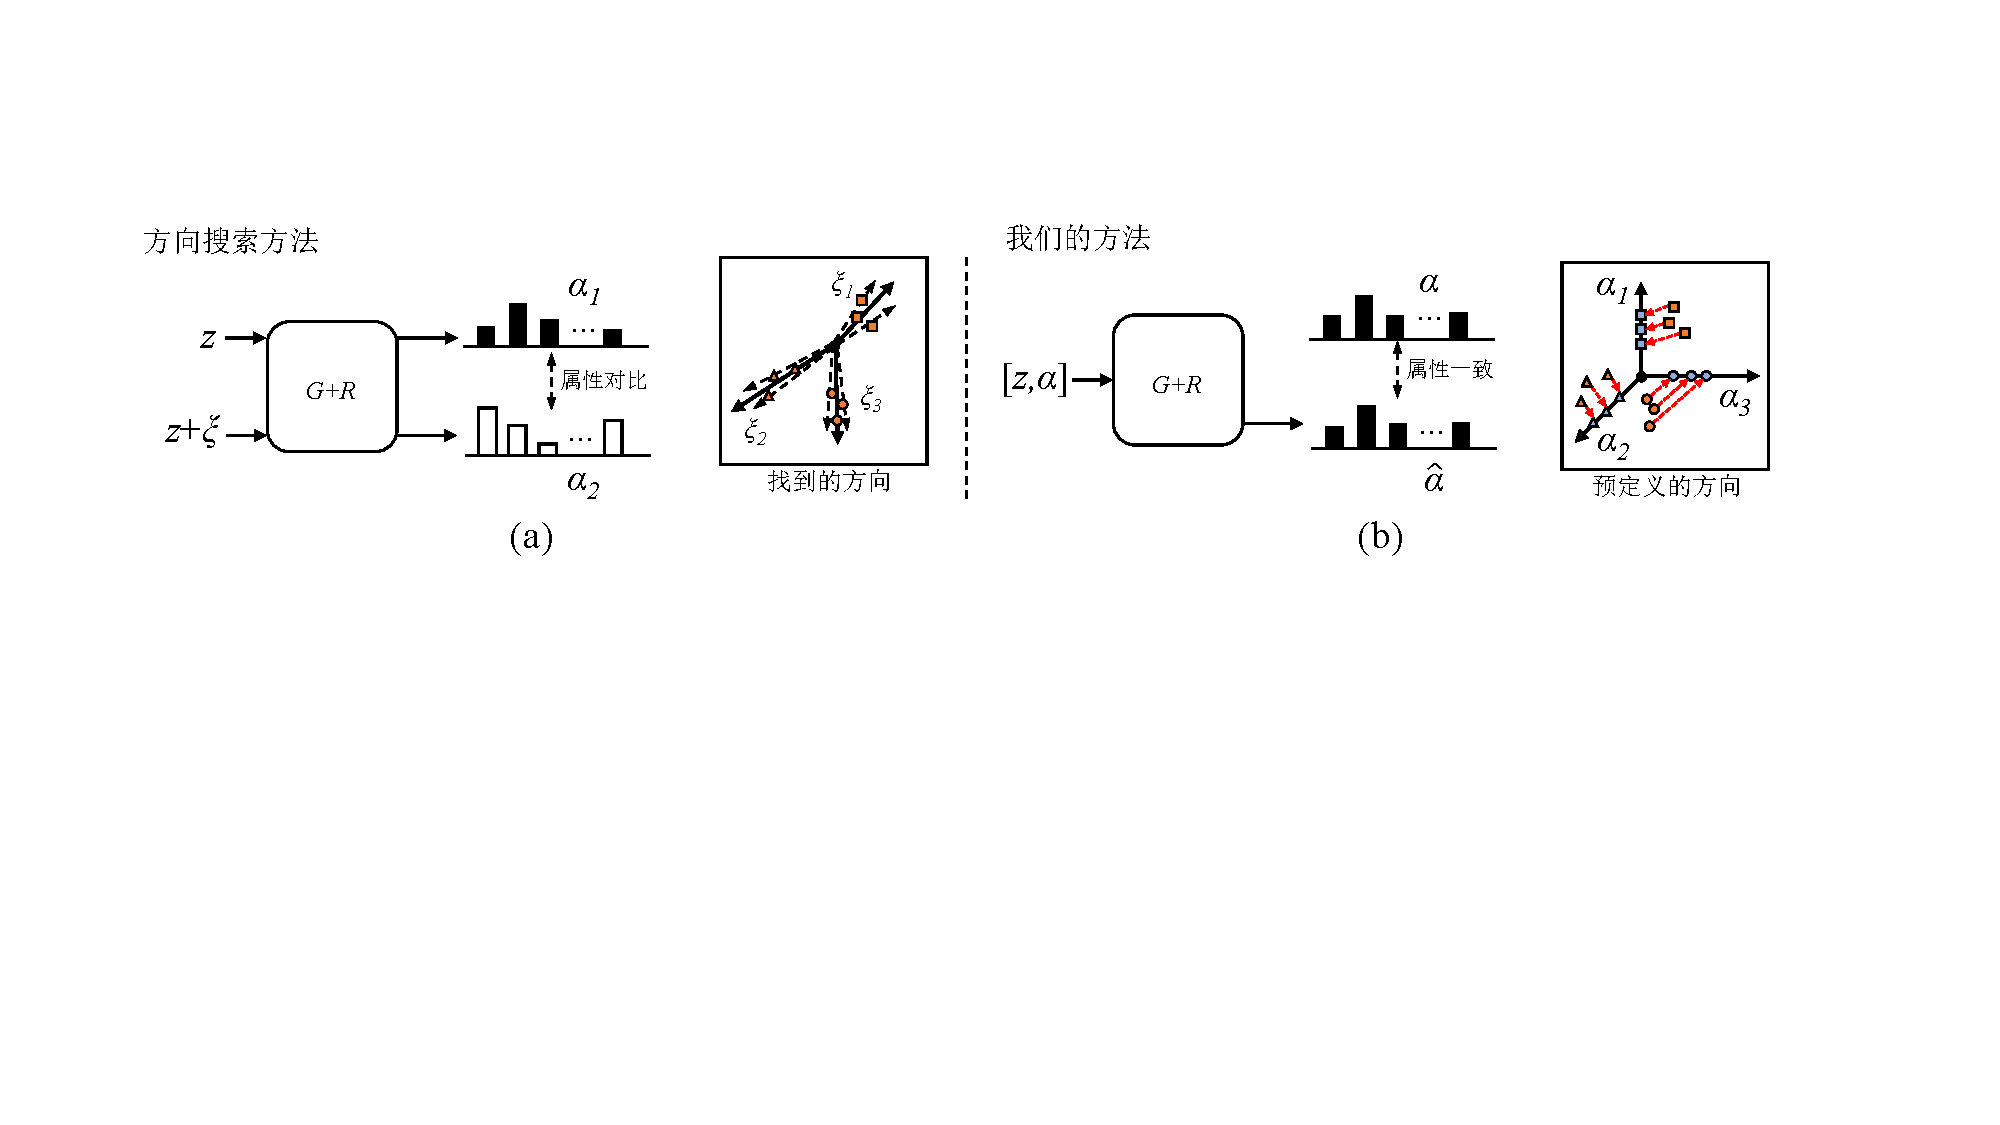
\includegraphics[width=1\linewidth]{figures/ACGAN/framework.pdf}
    \caption{方向搜索方法(左)和我们的方法(右)的框架}
    \label{fig:framework}
  \end{figure}

\subsection{连续属性标签量化}
% 形式化问题
% 对于给定的图片集$\{I_k\}_{k=1}^n \subset \mathbb{R}^{h \times w \times 3}$, 及其对应的属性集$\{y_k\}_{k=1}^n \subset \mathbb{R}^{d}$, 在这里$y_k$ is 0 for negtive or 1 for positive
假设我们有图片集 $\mathcal{D} = \{I_k\}_{k=1}^n \subset \mathbb{R}^{h \times w \times 3}$ 和属性集 $\mathcal{A} = \{y_k\}_{k=1}^n \subset \mathbb{R}^{d}$。 我们用 $\{I_k, y_k\}$ 表示数据集$\{\mathcal{D}, \mathcal{A}\}$种第 $k$ 张图片和其对应的属性标签。每个$y_k=[y_{k,1}, y_{k,2}, \cdot \cdot \cdot ,y_{k,N}]$, $y_{k,i}$的值是0或1, $N$是属性类别的数量。我们的目标是生成连续的伪标签 $\{\hat{y}_k\}_{k=1}^n$ 其中 $\{\hat{y}_k\}$ 包含 0 到 1 之间的连续值。

% 我们的想法是在$\mathcal{D}$上训练一个分类器,通过归一化分类器的置信度得到连续伪标签。
我们的想法是在$\{\mathcal{D}, \mathcal{A}\}$上训练一个由属性回归器$R_c$和一层$sigmoid$激活函数组成分类器,第$k$张图片分类置信度$x_{k}$的计算公式为:
\begin{equation}
     x_{k,i} = C(I_k) = sigmoid(R_c(I_k)),
\end{equation}
分类器通过二值交叉熵损失训练:
\begin{equation}
     \mathcal{L}_{BCE} = \sum_{k=1}^n \sum_{i=1}^d [y_{k,i} \cdot \log x_{k,i}+\left(1-y_{k,i}\right) \cdot \log \left(1-x_{k,i}\right)],
\end{equation}
最后通过归一化分类器的置信度得到连续伪标签。

如图~\ref{fig:quantization}(b)所示,我们通过公式:
\begin{equation}
     \hat{y}_{k,i} = \frac{R_c(I_k)_i - \min \limits_{1 \leq t \leq n}R_c(I_t)_i}{\max \limits_{1 \leq t \leq n}R_c(I_t)_i - \min \limits_{1 \leq t \leq n}R_c(I_t)_i},
     \label{eq3}
\end{equation}
归一化 $\{R_c(I_K)\}_{k=1}^n$,生成了连续的属性标签。

注意这里的$R_c(\cdot)$不包含$sigmoid$激活函数。我们使用$sigmoid$激活函数之前的值(即$R_c(I_K)$)来计算量化属性值的原因在于$sigmoid$是一个“软”的阶跃函数:
\begin{equation}
   \chi_{A}(x)=\left\{\begin{array}{ll}
      0 & \text { if } x \leq 0 \\
      1 & \text { if } x > 0,
      \end{array}\right.
\end{equation}
$sigmoid$会将$R_c(I_k)$推至接近于0或1的值。

现在我们有了连续属性标签集$\hat{\mathcal{A}}=\{\hat{y}_k\}_{k=1}^n$。我们将在新数据集$\{\mathcal{D}, \hat{\mathcal{A}}\}$上训练新的属性回归器$R$,并将其用于监督生成器训练。


\begin{figure}[!t]
  \centering
  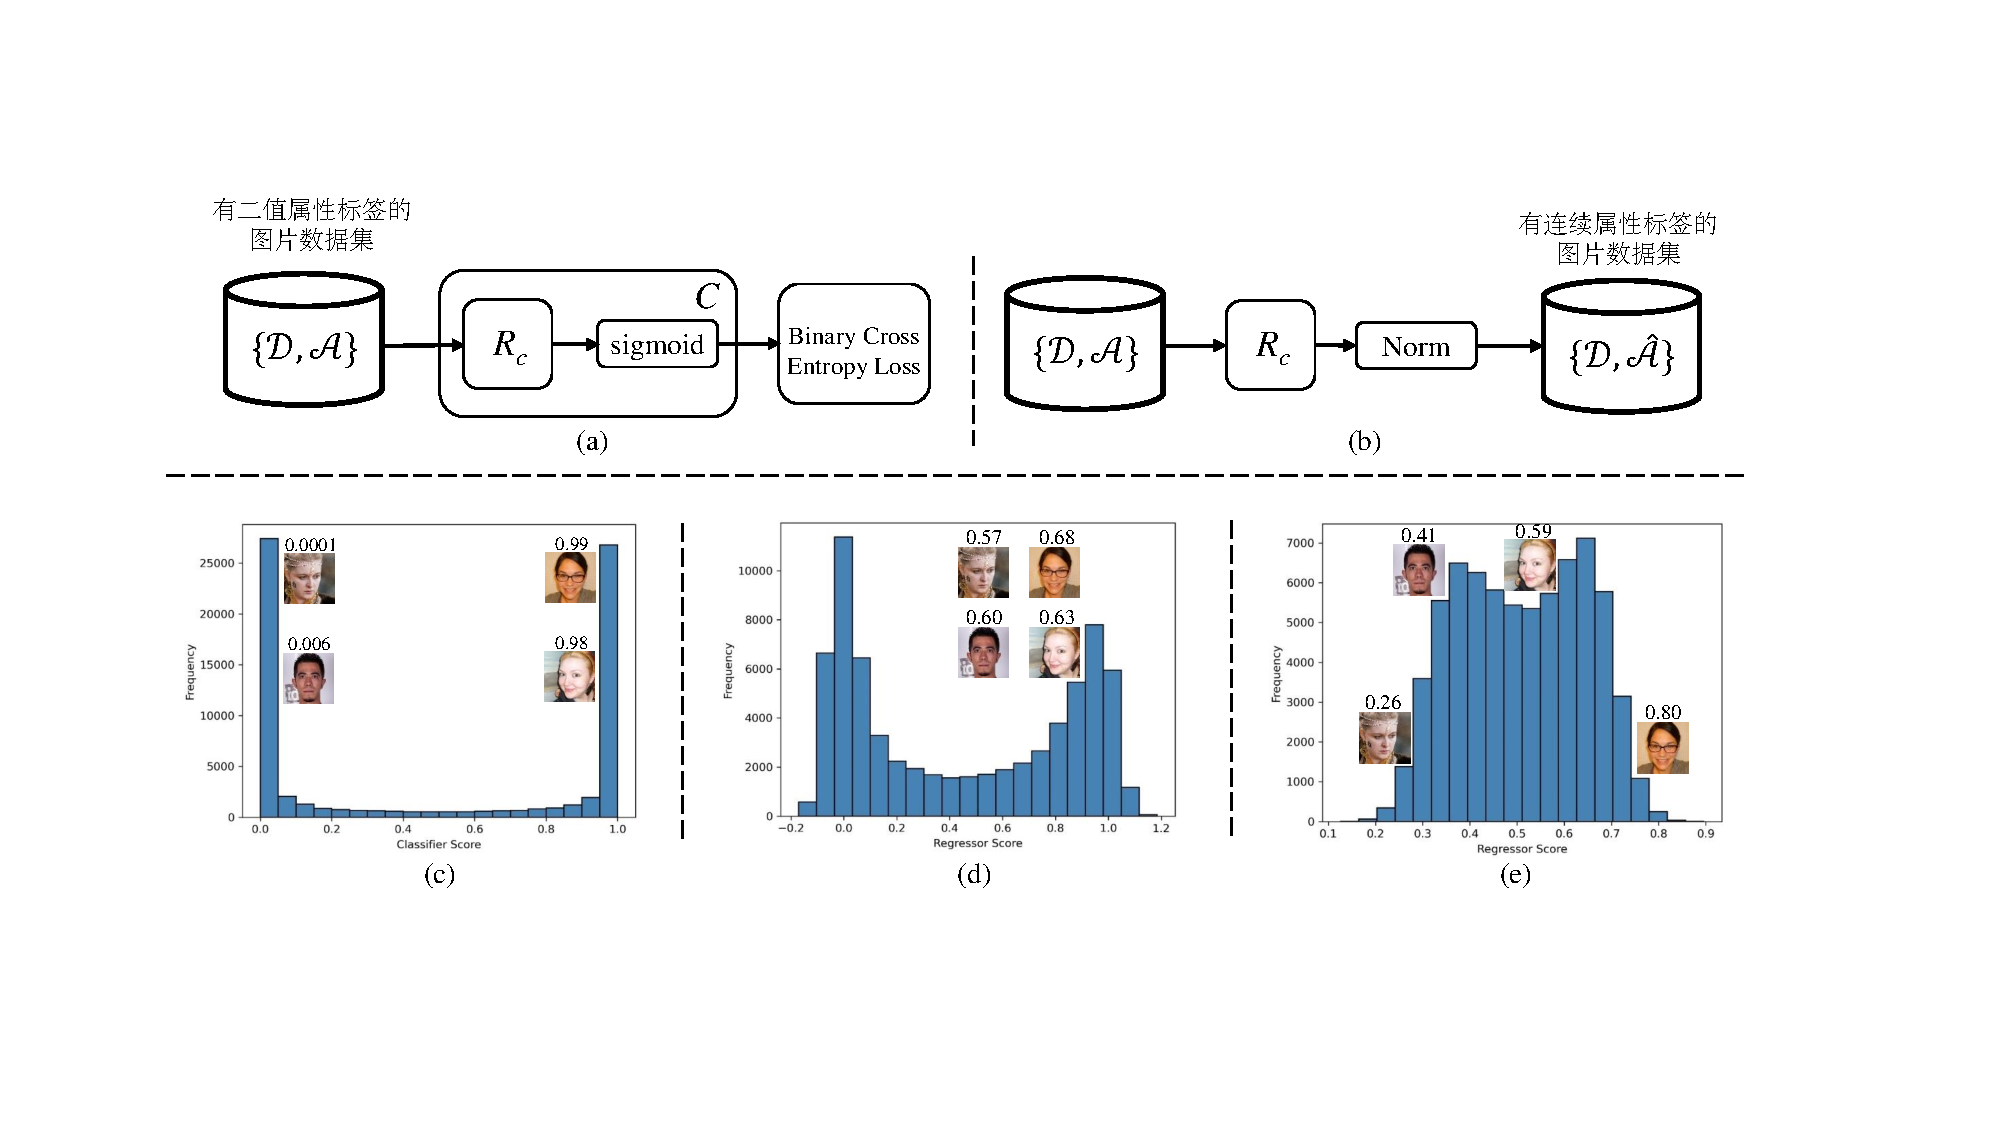
\includegraphics[width=1.0\linewidth]{figures/ACGAN/continue.pdf}
  % \caption{=连续属性生成。We first train an attribute classifier $C$ that consists of a continuous attribute regressor $R_c$ and a sigmoid layer as shown in (a) then we normalize outputs of $R_c$ as continuous labels as shown in (b). We collect attribute prediction values of classifier $C$ trained by $\mathcal{A}$, regressor $R_A$ trained by $\mathcal{A}$ and regressor $R$ trained by $\hat{\mathcal{A}}$ in (c), (d) and (e) respectively.}
  \caption{连续属性生成}
  % 我们首先训练属性分类器 $C$,它由一个连续属性回归器 $R_c$ 和一层 $sigmoid$ 组成,如(a)所示,然后我们将 $R_c$ 的输出归一化为连续标签,如(b)所示。 我们收集由 $\mathcal{A}$ 训练的分类器 $C$、$\mathcal{A}$ 训练的回归器 $R_A$ 和 $\hat{\mathcal{A}} 训练的回归器 $R$ 的属性预测值 $分别在(c)、(d)和(e)中。
  \label{fig:quantization}
\end{figure}

\subsection{属性一致性约束}
我们的ACGAN可以基于任意的非条件生成式对抗网络实现。ACGAN由3部分构成:生成器、判别器和属性回归器。我们将内容变量(高斯噪声,实现上相当于原来的隐变量)和属性变量共同作为网络的输入送入到生成器中,判别器的结构保持不变。属性回归器的作用是监督生成器的样本:生成器的训练目标不再仅仅是“骗过”判别器,还要满足生成样本的属性值与输入的属性变量一致。总之,在已有属性回归器的前提下,为了将任意的非条件生成式对抗网络改造成可以控制属性的ACGAN,仅需要做以下两点:1. 将生成器的输入扩充为隐变量和属性变量 2. 计算生成器的损失时加上属性一致性损失。
% \subsubsection{Overview} Our ACGAN can be implemented based on any unconditional GAN and is composed of 3 parts: a generator $G$, a discriminator $D$, and a pretrained attribute regressor $R$. Leaving the discriminator unchanged, the attribute code $\alpha$ and content code \emph{z} are fed into the generator as the inputs. $R$ is utilized to supervise the attributes of generated samples via attribute regression loss. The objective of the generator is no longer just to "deceive" the discriminator, but also to satisfy the attribute consistency, i.e., the attribute of the generated samples equal to the input attribute code. In short, in order to transform any unconditional GAN into ACGAN, only two changes need to be implemented: (1) decomposing the input values into content values and attribute values; (2) adding attribute regression loss.

\subsubsection{属性一致性损失}
ACGAN能够控制生成样本属性的关键之处在于在训练阶段生成样本的属性受到属性回归器的约束,这正是通过属性一致性损失(Attribute Consistency Loss)实现的。
% The key point to control the attributes of the generated samples is that the attributes of the generated samples are constrained by the attribute regressor in the training phase. This is achieved through minimizing $l_2$-norm between input attribute code $\alpha$ and predicted attribute $R(G(z|\alpha))$.% i.e., $\|R(G(z|\alpha)) - \alpha\|_2$.
% % \begin{equation}
% %      L_{Reg} =  \mathbb{E}_{z \sim \mathcal{N}(0,1), a \sim \mathcal{U}(0,1)}\|R(G(z|a)) - a\|_2
% % \end{equation}
% \begin{equation}
%      \|R(G(z|\alpha)) - \alpha\|_2
% \end{equation}

如何在训练阶段采样属性变量$\alpha$?我们在这里提供两种采样方式:1)从连续标签集$\hat{\mathcal{A}}$中采样 2)从均匀分布$\mathcal{U}(0,1)$采样。
当数据集中的属性在语义上存在耦合时,某些属性值的组合可能是不合理的。以CelebA数据集为例,山羊胡(goatee)和男性(male)这两种属性是高度耦合的,从常识上判断,男性为0但山羊胡的属性为1的组合是不合理的,
% How to sample $\alpha$ in the training phase? We investigate two sampling strategies: 1) sampling from the pseudo-label set $\hat{\mathcal{A}}$, 2) sampling from a uniform distribution $\mathcal{U}(0,1)$. 
% When attributes in $\mathcal{A}$ are semantically tangled, the combination of certain attribute values may be unreasonable. Taking CelebA dataset~\cite{celeba} as an example, the two attributes \textit{goatee} and \textit{male} are highly tangled. This combination is unreasonable where \textit{goatee} is 1 and \textit{male} is 0.

考虑到 $\hat{\mathcal{A}}$ 中的每个伪标签对应于 $\mathcal{D}$ 中的真实图像,第一种策略可以保证采样的 $\alpha$ 是合理的。
此时属性一致性损失$\mathcal{L}_{cons}$可形式化为公式:
% Considering that each pseudo label in $\hat{\mathcal{A}}$ corresponds to a real image in $\mathcal{D}$, the first strategy can guarantee $\alpha$ is reasonable.
% Attribute-consistent loss can be formulated as:
\begin{equation}
   \mathcal{L}_{cons}(G, R)  =  \mathbb{E}_{z \sim \mathcal{N}(0,1), \alpha \sim \hat{\mathcal{A}}}\|R(G(z|\alpha)) - \alpha\|_2
\end{equation}

至于第二种策略,我们可能会从 $\mathcal{U}(0,1)$ 中采样不合理的 $\alpha$,但是与第一种相比,这种采样策略有两个不可或缺的优势:

1) $\hat{\mathcal{A}}$ 中的属性值组合分布不均匀。让我们假设 $\alpha$ 中的每个变量都服从正态分布 $\mathcal{N}(0,1)$。如果我们直接从 $\hat{\mathcal{A}}$ 中采样 $\alpha$,中间属性值(接近 0.5)的采样概率最高,而采样极端属性值(接近 0 或 1)的概率) 会非常小。这实际上与我们的目标相矛盾:当输入属性从 0 线性变化到 1 时,我们希望 ACGAN 能够线性地生成相应属性值的样本。在这个过程中,我们平等对待中性属性值和极端属性值,因此从 $\mathcal{U}(0,1)$ 采样是一个更好的策略。

2) $\hat{\mathcal{A}}$ 中的样本可能有限。请注意,$\alpha$ 位于高维空间 $\mathbb{R}_N$ 中。当我们从 $\hat{\mathcal{A}}$ 中采样时,若假设${\mathcal{A}}$中共有$n$个样本,那么整个采样过程相当于在 $\mathbb{R}_N$ 中采样 $n$ 个点。如果我们采用第二种策略,采样点的数量取决于我们训练 ACGAN 的迭代次数,该次数远大于 n。
%As for the second strategy, we may sample unreasonable $\alpha$ from $\mathcal{U}(0,1)$, but this sampling strategy has two indispensable advantages compared to the first one: 

%1) Combination of attribute values in $\hat{\mathcal{A}}$ is quite biased. Let us assume that each variable in $\alpha$ obeys normal distribution $\mathcal{N}(0,1)$. If we directly sample $\alpha$ from $\hat{\mathcal{A}}$, the medium attribute value (close to 0.5) has the highest sampling probability, while the probability of sampling extreme attribute value (close to 0 or 1) will be very small. This actually contradicts our goal: when the input attribute changes linearly from 0 to 1, we wish ACGAN can linearly generate samples of the corresponding attribute value. In this process, we treat neutral attribute values and extreme attribute values equally, so sampling from $\mathcal{U}(0,1)$ is a better strategy.

%2) The samples in $\hat{\mathcal{A}}$ may be limited. Note that $\alpha$ lies in a high-dimensional space $\mathbb{R}_N$. It is insufficient to sample $n$ points in $\mathbb{R}_N$, but this is exactly what we do when sampling from $\hat{\mathcal{A}}$.If we adopt the second strategy, the number of sampled points depends on the number of iterations we train ACGAN, which is much larger than n.

一般情况下属性变量从均匀分布采样即可,此时属性一致性损失可以被形式化为:

% Generally, sampling $\alpha$ from $\mathcal{U}(0,1)$ is a more universal strategy. Attribute regression loss can be formulated as:
\begin{equation}
     \mathcal{L}_{cons}(G, R)  =  \mathbb{E}_{z \sim \mathcal{N}(0,1), \alpha \sim \mathcal{U}(0,1)}\|R(G(z|\alpha)) - \alpha\|_2
\end{equation}

% LGAN是
\subsubsection{网络总损失}
引入 $R$ 实现的属性一致性损失后,我们需要做的就是在原始 GAN 损失的基础上加入属性回归损失:
% After introducing the attribute regression loss implemented by $R$, all we need to do is adding attribute regression loss to original GAN loss:
\begin{equation}
     \min _{G} \max _{D} V(D, G, R) = \mathcal{L}_{GAN}(G, D) + \lambda \mathcal{L}_{cons}(G, R),
     \label{overall}
\end{equation}
其中 $\mathcal{L}_{GAN}$ 是原始对抗损失,例如 WGAN~\cite{wgan} 中的 Wasserstein 损失或 LSGAN~\cite{lsgan} 中的最小二乘损失,$\lambda$ 是 $L_{cons}$的平衡超参数。
% where $\mathcal{L}_{GAN}$ is the original adversarial loss such as Wasserstein loss in WGAN~\cite{wgan} or least squares loss in LSGAN~\cite{lsgan}, $\lambda$ is a hyper parameter balancing $L_{Reg}$.

\subsubsection{ACGAN的训练算法}
我们在算法 ~\ref{al:acgan}描述了ACGAN的训练流程,可以看到与训练非条件GANs的最大区别在于训练过程中加入的属性一致性损失。

\begin{algorithm}[H]
\caption{ACGAN的训练算法}
\label{al:acgan}
\textbf{输入}: 预训练属性回归器 $R$, 生成器 $G$,判别器 $D$, 批大小 $K$, 最大迭代次数 $M$, 图片数据集 $Q$, $G$的学习率$\mu_G$ 和 $D$的学习率 $\mu_D$\\
\textbf{参数}: $\theta_G$, $\theta_D$\\
\textbf{输出}: 判别器$D$和属性一致的生成器 $G$\\
\begin{algorithmic}[1] %[1] enables line numbers
\STATE 用参数 $\theta_G$ 初始化$G$,用参数 $\theta_D$ 初始化$D$,当前迭代次数$iteration=0$
\WHILE{$iteration \leq M$}
\STATE 采样 $z \sim \mathcal{N}(0,1), \alpha \sim \mathcal{U}(0,1)$;\\
    \STATE 生成 $I=G([z,\alpha])$;\\
    \STATE 计算 $\hat{\alpha} = R(I)$;\\
    \STATE 计算 $L=\mathcal{L}_{GAN}(G,D) +  \lambda \mathcal{L}_{Cons}(\alpha, \hat{\alpha})$;\\
    \STATE 更新 $\theta_G = \mu_G * \partial{L}/\partial{\theta_G}$;\\
    \STATE 更新 $\theta_D = \mu_D * \partial{L_{GAN}}/\partial{\theta_D}$;
\ENDWHILE
\STATE \textbf{return} $\theta_G$ and $\theta_D$
\end{algorithmic}
\end{algorithm}


\section{实验}

\subsection{实验细节}
本文在人脸合成和自然场景合成两个场景做了实验。 在本节中,本文将介绍 $C$ 和 $R$ 的基本模型和架构,然后分别描述这两个场景的实现细节。
% We conduct experiments on face synthesis and natural scene synthesis. In this section, we will introduce base model and architecture of $C$ and $R$, then describe implementation details in these two scenarios separately.

\subsubsection{基本模型} 
对于人脸合成场景,本文使用StyleGAN2~\cite{stylegan2} 实现了ACGAN;对于自然场景合成场景,本文则使用了轻量级 GAN~\cite{lwgan}来实现ACGAN。属性变量$\alpha$ 分别拼接在 轻量级 GAN 的 $z$ 和 StyleGAN2 的 $w$ 后面。
% We implement the proposed ACGAN based on light-weight GAN~\cite{lwgan} and StyleGAN2~\cite{stylegan2}. Due to the heavily computing cost of Stylegan2, we halve number of channels of convolution layer in each style block of Stylegan2. We term this more light weight Stylegan2 as Stylegan2-mini, which is adopted as the basic generative model  in the face synthesis experiments. The attribute code $\alpha$ is concatenated with $z$ for light-weight GAN and $w$ for StyleGAN2.

\subsubsection{$C$和$R$的结构}
本文采用 ResNet-50~\cite{resnet} 作为分类器 $C$ 和回归器 $R$ 的骨干网络,并且用维度为$N$的全连接层替换最后一个全连接层,这里的$N$为属性类别的数量,例如在CelebA数据集~\cite{celeba}数据集中$N=40$。 除$C$包含最后一层$sigmoid$外, $C$ 和 $R$ 共享相同的网络结构。 本文在 CelebA 数据集上训练分类器 $C$,达到 $96.05\%$ 的分类准确度。在 $\hat{\mathcal{A}}$ 上训练的回归器在验证集上的最小均方误差(MSE)达到 $0.0337$ ,在自然场景数据集~\cite{scenedataset} 上训练的回归器的MSE达到 $0.0142$。
% We adopt ResNet-50~\cite{resnet} as the backbone architecture of classifier $C$ and regressor $R$. The last fully connected layer is replaced by a new one with the dimension of $N$ corresponding to attribute categories. We isolate $sigmoid$ from attribute classifier $C$, so $C$ and $R$ can share the same network architecture. We train the classifier $C$ on CelebA dataset, which achieves $96.05\%$ of classification accuracy. The regressor trained on $\hat{\mathcal{A}}$ reaches validation MSE of $0.0337$ and the regressor trained on Transient Attribute Database~\cite{scenedataset} and reaches validation MSE of $0.0142$.

\subsubsection{数据集}
对于人脸合成,我们在CelebA 数据集~\cite{celeba}上训练了属性分类器和回归器。这是一个大规模的人脸属性数据集,由超过 20万张名人照片组成。每张图像有 40 种属性标注,分辨率为 $178\times218$。 我们的 ACGAN 模型在 Flickr-Faces-HQ (FFHQ)~\cite{stylegan} 数据集上进行训练,该数据集由$70,000$的高质量图像组成,分辨率为$1024\times1024$,并且在年龄、人种和图像背景方面包含相当大的变化。 FFHQ上训练的模型能够生成更真实的图像。
% For face synthesis, the facial attribute knowledge is learned from CelebA dataset~\cite{celeba}, which is a large-scale face attributes dataset consists of more than 200K celebrity images, each with 40 attribute annotations at $178\times218$ resolution. Our ACGAN model is optimized on Flickr-Faces-HQ (FFHQ)~\cite{stylegan} dataset, which consists of $70,000$ high-quality images at $1024\times1024$ resolution and contains considerable variation in terms of age, ethnicity and image background. FFHQ enables the model to generate high-fidelity images. 

% We select all 40 attributes for training as only a few attributes are mutually entangled.
对于自然场景合成,回归器 $R$在 Transient Attribute Database~\cite{scenedataset} 上训练。 由于该数据集具有介于 $0$ 和 $1$ 之间的连续属性值,因此没有必要训练属性分类器 $C$。 受EnjoyEditing~\cite{iclr2021}的启发,我们从Place数据集~\cite{place}和SUN数据集~\cite{sun}中选择了40,726张与自然场景相关的图片来扩展Transient Attribute数据集,并利用这个增强的自然场景数据集来训练我们的ACGAN模型。
% For natural scene synthesis, the natural attribute knowledge is learned from Transient Attribute Database~\cite{scenedataset} for regressor $R$. Since this dataset has continuous attribute values between 0 and 1, it is unnecessary to train an attribute classifier $C$. Motivated by \cite{iclr2021}, we selected 40,726 pictures related to natural scenes from Place dataset~\cite{place} and SUN dataset~\cite{sun} to expand the Transient Attribute dataset, and utilized this augmented natural scene dataset to optimize our ACGAN model. 

% Unfortunately, lots of attributes are tangled, e.g., "daylight" and "night", "summer" and "winter". To avoid problem of tangled attributes discussed in Sec.\ref{section-31}, we select 5 attributes: "night", "clouds", "fog", "winter" and "sunny".

\subsubsection{其他实现细节}
我们将用于平衡属性回归损失的超参数 $\lambda$ 设置为所选属性的数量,在人脸合成场景$\lambda=40$,自然场景合成下$\lambda=5$。 $C$ 和 $R$ 均由 Adam~\cite{adam} 优化器训练,学习率为 0.0001。另外,我们使用单张 Titan RTX 进行所有实验。
% We set hyperparameter $\lambda$ to denote the number of selected attributes for balancing attribute regression loss, i.e., $\lambda=40$ for face synthesis and $\lambda=5$ for natural scene synthesis.  Both $C$ and $R$ are trained by an Adam optimizer with a learning rate of 0.0001. We use a single Titan RTX for all experiments.

\subsection{人脸属性编辑相关实验}
为了表示方便,我们统一使用“+属性名”表示增强该属性,相对应的,“-属性名”表示减弱该属性。

\subsubsection{定性比较}
本节将定性评测ACGAN单种属性和多种属性的编辑效果,并将其与两种有监督隐空间编辑方法进行比较:InterFaceGAN~\cite{interfacegan} 和 EnjoyEditing~\cite{iclr2021}。 截止文本撰写为止,EnjoyEditing的官方代码还没有公布,感谢他们简洁的框架,我们重新实现了他们的工作。为了公平地与这两种方法比较,我们采用文献~\cite{image2stylegan}的逆映射(Inversion)方法将一张真实图像编码到 StyleGAN2 的隐空间中,以比较同一图像上的属性编辑性能。
% We evaluate the attribute controllability on single and multiple attributes, and compare our method with two advanced supervised methods: InterFaceGAN~\cite{interfacegan} and EnjoyEditing~\cite{iclr2021}. Since the official code of EnjoyEditing is not released yet, we re-implement it by ourselves thanks to their concise framework. To fairly compare the performance of the two methods, we adopt \cite{image2stylegan} to encode one real image into the latent space of StyleGAN2, and compare the attribute editing performance on the same image.

图~\ref{fig:face} 展示了单属性编辑(b,c)和多属性编辑(d,e,f)的结果,Inversion表示逆映射方法得到的生成图像。 对于+刘海,我们的 ACGAN 是唯一成功添加刘海的方法;而 InterFaceGAN 和 EnjoyEditing 只是将发际线向前移动了一点。 对于+胖,我们的 ACGAN 实现了最精确和最清晰的编辑结果;InterFaceGAN的结果比原图要老;而EnjoyEditing的结果在增强胖属性方面不明显。
% Fig.~\ref{fig:face} shows results of single attribute editing (b, c) and multi attributes editing (d, e, f). For adding bangs, our ACGAN is the only method that adds bangs successfully, while InterFaceGAN and EnjoyEditing just move Hairline a little forward. For adding chubby, our ACGAN achieves most precised and distangled editing result. The result of InterFaceGAN is older than the original image, and the result of EnjoyEditing is not obvious at adding chubby.

对于多属性编辑评估,我们的 ACGAN 可以在不改变图像身份的情况下同时修改多种属性,如图~\ref{fig:face}所示。从编辑$1$种属性到$7$种属性,我们的ACGAN(第一行)展示出了非常精确的编辑效果。这$7$种属性包括:笑、胖、黑发、金发、口红、大鼻子 和 白皮肤。相比之下,两个基准方法无法添加某些属性或更改了不相关的属性。 InterfaceGAN 在图~\ref{fig:face}(c) 和 (d) 中涉及多属性编辑时对逆映射图像(Inversion)几乎没有做出什么改变。 当-棕头发时,EnjoyEditing 显然会将头发变得更显金色,纹理细节也变得更加模糊,从而导致人物整体外观更差,如图~\ref{fig:face}(d) 所示。
% For multiple attributes editing evaluation, our ACGAN can modify multiple attributes simultaneously without changing the image identity, as shown in Fig.~\ref{fig:face}. In contrast, the baselines fail to add certain attributes or change irrelevant attributes that should be preserved. InterfaceGAN does not make much changes to the inverted image when it comes to multiple attribute editing in Fig.~\ref{fig:face}(c) and (d). EnjoyEditing obviously changes hair color to be blonder when we decrease the \textit{blond hair} attribute. The texture details also become more blurred, which leads to a worse qualitative appearance as shown in Fig.~\ref{fig:face}(d).

\begin{figure}[!t]
     \begin{center}
        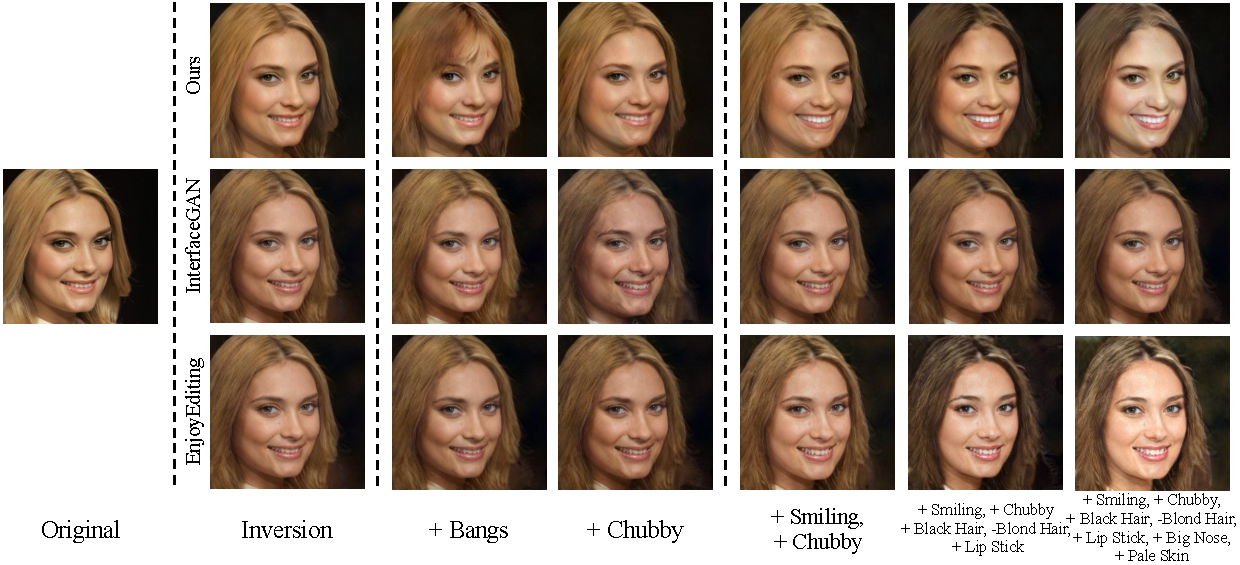
\includegraphics[width=1\linewidth]{figures/ACGAN/FaceMulti_center.pdf}
     \end{center}
     % \caption{Single attribute editing and multi attributes editing evaluation. On the first row, the results generated by our ACGAN are tremendously precise even for enhancing or reducing from $1$ to $7$ attributes including \textit{smiling, chubby, black Hair, blond Hair, lip stick, big Nose} and \textit{pale skin}. Please zoom-in for details.}
     \caption{单属性和多属性编辑的比较}
     \label{fig:face}
\end{figure}

\subsubsection{定量比较}
在本节我们提供两种定量方法,分别基于分类器评测与用户调研,来比较我们的方法与基准方法的性能差异。

为了评估属性编辑的准确性,我们统计了每种属性编辑的成功率和编辑一种属性时其他属性保持不变的的比例(我们称为保留率),这些指标均由预训练的分类器$C$计算得到。对于成功率,我们随机生成5000张图像并编辑所有这些图像的每种属性。我们的方法在所有属性中实现了 $84.13\%$ 的平均成功率,远高于 En​​joyEditing 的 $26.91\%$。在保留率的评估中,对于每种属性,我们收集5000张可以成功编辑该属性的图像,并统计其他未更改的属性比例。我们的方法实现了 $81.59\%$ 的平均保留率,这也优于EnjoyEditing。 图~\ref{fig:histogram} 具体比较了每种属性编辑的成功率和保留率。由于空间有限,并考虑到EnjoyEditing比InterfaceGAN的性能更好,本文只比较我们的方法和EnjoyEditing。我们的方法在大多数属性上的成功率和保留率达到了最高。
% To evaluate the attribute editing accuracy, we report the success rate of each attribute editing and the retention rate of irrelevant attributes while editing one attribute. These metrics are measured by a pretrained classifier. For success rate, we randomly sample $5,000$ images and edit each attribute for all these images. Our method achieves $84.13\%$ of averaged success rate among all the attributes, which is much higher than $26.91\%$ of EnjoyEditing. In the evaluation of retention rate, for each attribute, we generate $5,000$ images that can successfully edit this attribute and measure the other unchanged attributes. Our method achieves $81.59\%$ of averaged retention rate, which is also superior than EnjoyEditing. Fig.~\ref{fig:histogram} presents the comparisons on each attribute. Our method achieves the superiority performance on all the attributes for success rate and advanced accuracy on most attributes for retention rate. We also provide multiple attribute editing comparisons in the supplementary material.

% 柱状图
\begin{figure}[!t]
    \begin{center}
         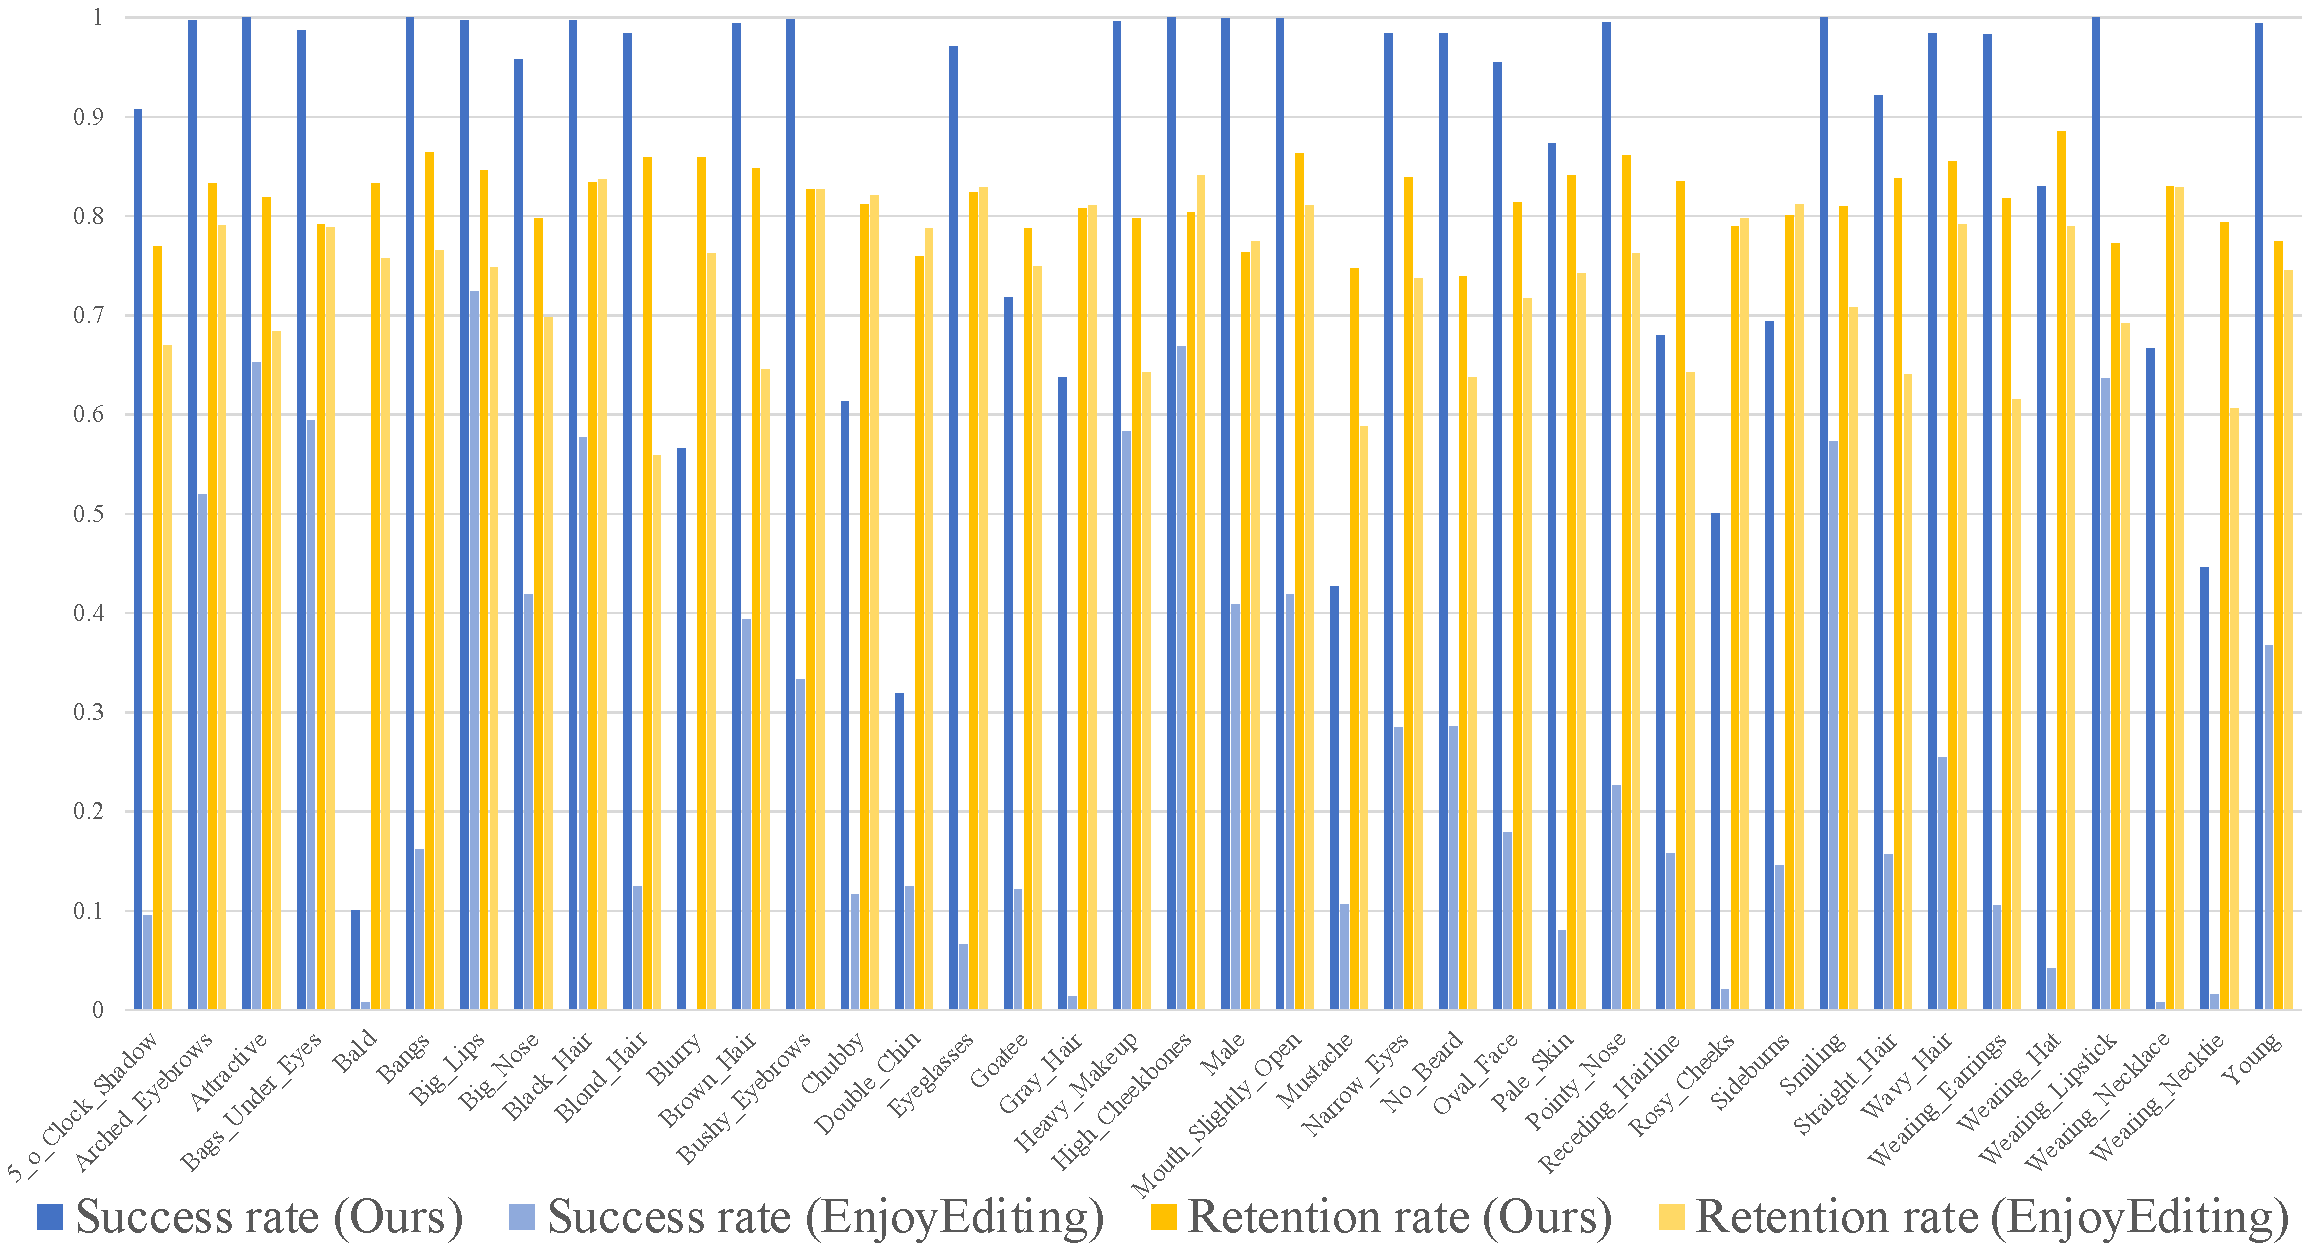
\includegraphics[width=1\linewidth]{figures/ACGAN/excel_histogram.pdf}
    \end{center}
    % \caption{Comparisons of attribute editing accuracy. EnjoyEditing achieves better performance than InterfaceGAN, we only compare our method with EnjoyEditing due to limited space. Please zoom-in for details.}
    \caption{单属性编辑成功率和保留率的的比较}
    \label{fig:histogram}
\end{figure}

我们通过用户调研进一步评估复合属性编辑分数 $\delta$ (属性编辑的成功率)和身份保留分数(即属性编辑的过程中人物身份是否发生变化,是否变成了另外一个人) $\epsilon$。对于我们的 ACGAN,我们首先生成所有属性变量 $0.5$ 的 图像$I_0$,然后我们在原属性变量上减少年龄、黑发、棕发 并增加 灰发(大部分属性值的变化量为$0.3$ )生成 $I_1$。注意属性值是累加的,所以我们在$I_1$的属性代码上增强微笑、浓眉和大鼻子属性,生成$I_2$。 我们生成 $I_3$ 的方式与生成$I_2$时类似。 对于基准方法~\cite{interfacegan}~\cite{iclr2021},我们通过随机抽样隐变量生成$I_0$,并通过隐空间向量算法,以类似属性变化累加的方式生成$\{I_1, I_2, I_3\}$。

我们在图~\ref{fig:questionnaire}中展示了一些生成的人脸图像序列$\{I_0, I_1, I_2, I_3\}$。对于三种不同方法的,我们要求用户回答以下问题:

\begin{enumerate}
\item 图像对 $\{I_0, I_1\}$ 是否满足“更年老”、“更少黑头发”、“更少金发”、“更多白头发”的属性变化?

\item 忽略上题描述的属性变化, $\{I_0, I_1\}$ 中的人物是否是同一个人?

\item 图像对 $\{I_1, I_2\}$ 是否满足“更多微笑”、“更浓密的眉毛”和“更大的鼻子”的属性变化?

\item 忽略上一个问题描述的属性变化,图像对 $\{I_1, I_2\}$ 中的人物是否是同一个人?

\item 图像对$\{I_2, I_3\}$是否满足“更瘦”、“更少双下巴”、“脸更圆”的属性变化?

\item 忽略上题描述的属性变化,图像对 $\{I_2, I_3\}$ 中的人物是否是同一个人?
\end{enumerate}

% For our ACGAN, we first generate $I_0$ with all attributes set to $0.5$, then we reduce \textit{young}, \textit{black hair}, \textit{blond hair} and increase \textit{gray hair} (by $0.3$ mostly) on attribute code of $I_0$ to generate $I_1$. Note that the attribute values are added in an accumulative manner, so we add \textit{smile bushy} and \textit{big nose} on attribute code of $I_1$ to generate $I_2$. The way we adopt to generate $I_3$ is similar to $I_2$. For baselines~\cite{interfacegan}~\cite{iclr2021}, we generate $I_0$ by randomly sampling latent code, and generate $\{I_1, I_2, I_3\}$ through latent space arithmetic but also in an accumulative manner.

% We present some generated face image sequences $\{I_0, I_1, I_2, I_3\}$ in Fig.~\ref{fig:questionnaire}. For each pair in $\{(I_0, I_1), (I_1, I_2), (I_2, I_3)\}$ of all three different methods, we have the following questions:

% \begin{enumerate}
% \item Does the image pair $\{I_0, I_1\}$ satisfy the property changes of "older", "less black hair", "less blond hair" and "more gray hair"?

% \item Ignoring the attribute changes described in the previous question, does the image pair $\{I_0, I_1\}$ have the same identity?

% \item Does the image pair $\{I_1, I_2\}$ satisfy the property changes of "more smiling", "more bushy eyebrows" and "bigger nose"?
% attribute
% \item Ignoring the property changes described in the previous question, does the image pair $\{I_1, I_2\}$ have the same identity?

% \item Does the image pair $\{I_2, I_3\}$ satisfy the property changes of "less chubby", "less double chin" and "less oval face"?

% \item Ignoring the attribute changes described in the previous question, does the image pair $\{I_2, I_3\}$ have the same identity?
% \end{enumerate}

\begin{figure}[!t]
    \begin{center}
         \includegraphics[width=1\linewidth]{figures/ACGAN/questionnaire_new.pdf}
    \end{center}
    \caption{用户问卷样本}
    \label{fig:questionnaire}
\end{figure}

用户调研结果如表~\ref{tb:userstudy}所示。每个单元格中的两个数字分别为属性编辑得分和加权身份保持得分。A组是\{-年轻,-黑色头发,-金色头发,+灰色头发\},B组是\{+微笑,+浓密眉毛,+大鼻子\},C组是-\{-胖,-双下巴,-鹅蛋脸\}。对于身份保留,考虑到这个分数只有在满足属性编辑时才有意义,我们提出了加权身份保留分数 $\epsilon_w = \delta * \epsilon$。 每个单元格中的两个数字分别是 $\delta$ 和加权的 $\epsilon_w$。 我们的方法在编辑精度和加权身份保留两方面均显示出在复合属性编辑上的优越性。 
% We further evaluate composite attributes editing score $\delta$ and identity preserving score $\epsilon$ by user study.  For identity preserving, this score is meaningful only when attributes editing is satisfied. Based on this, we propose weighted identity preserving score $\epsilon_w = \delta * \epsilon$. The evaluation results are reported in Table.\ref{tb:userstudy}. The two numbers in each cell are $\delta$ and weighted $\epsilon_w$, respectively. Our method shows superiority on composite attributes editing in both editing precision and weighted identity preserving evaluations. We provide more details of the user study in supplementary material.

\begin{table}
    \caption{基于用户调研的复合属性编辑的定量评价}
    % \caption{Quantitative evaluation of composite attributes editing. The two numbers in each cell are attribute editing score and weighted identity preserving score respectively. GROUP A is \{-Young, -Black Hair, -Blond Hair, +Gray Hair\}, GROUP B is \{+Smile, +Bushy Eyebrows, +Big Nose+\}, GROUP C is \{-Chubby, -Double Chin, -Oval Face\}.}
    \renewcommand\arraystretch{0.8}
        \begin{center}
        % {lC{3.4cm}C{3.3cm}C{2.8cm}}
        \begin{tabular}{cccc}
        \toprule
        & \makecell[c]{A组} & \makecell[c]{B组} & \makecell[c]{C组}\\
        & $\delta$ \space\space\space\space\space\space $\epsilon$  & $\delta$ \space\space\space\space\space\space $\epsilon$  & $\delta$ \space\space\space\space\space\space $\epsilon$ \\
        \midrule
        InterFaceGAN &$45.4$ \space\space $34.0$ &$52.8$\space\space $35.5$&$60.3$ \space\space $40.6$ \\
        \specialrule{0em}{1pt}{1pt}
        EnjoyEditing &$65.9$ \space\space $49.1$ &$76.0$ \space\space $59.1$&$58.9$ \space\space $46.6$ \\
        \specialrule{0em}{1pt}{1pt}
        Ours &$\textbf{87.7}$ \space\space $\textbf{70.6}$ &$\textbf{84.3}$ \space\space $\textbf{68.5}$&$\textbf{85.9}$ \space\space $\textbf{65.0}$ \\
        \bottomrule
        \end{tabular}
        \end{center}
        \label{tb:userstudy}
\end{table}


\subsubsection{所有属性的编辑}
以前的有监督的隐空间编辑方法仅能在CelebA 数据集的少数 ($<$4) 种属性起作用。我们的方法在这方面取得了很大进展,能够编辑生成样本的所有 40 种属性。具体的做法是,我们将所有属性值都初始化为 $0.5$,对于每种属性编辑,只需将该属性值修改为1,同时保持其他属性值和原始内容值不变。 图~\ref{fig:40Attributes}展示了CelebA 数据集中所有 40 种属性的编辑样本。
我们的模型能够很好地解耦大多数属性,除了四个“穿戴性质”的属性:戴项链、戴领带、戴耳环和戴着帽子,这证明了所提出的正交属性空间的有效性,
在分析这些穿戴属性的比例时,我们发现对这些属性的编辑失败并不是由数量引起的。例如,同为穿戴性质属性,眼镜在数量比例上可与其他四种穿戴性质接近,但属性编辑的结果却合理的多。这可能是因为眼镜在面部的大小和位置是相对固定的,而其他穿戴性质属性则不是,这使得“眼镜”的属性编辑比其他穿戴性质属性的编辑更容易学习。
% Previous supervised direction searching methods are only compatible with few ($<$ 4) attributes of the CelebA dataset. Our method has made great progress in this regard, being able to edit all the 40 attributes of the generated samples. Specifically, all the attribute values are initialized to $0.5$. For each attribute editing, we simply modify the editing attribute value to 1 while keep other attribute values and original content values unchanged. Fig.~\ref{fig:40Attributes} demonstrates the effectiveness of the proposed attribute orthogonal space, which empowers our model to well disentangle most attributes except for four "\textit{wearing}" attribute: wearing necklace, wearing necktie, wearing earrings and wearing hat.
% While analyzing the proportion of these wearable attributes, we found that the failure editing on these attributes is not caused by quantity. For instance, as a wearable attribute, eyeglasses are comparable to the other four wearable attributes in the quantity proportion but present reasonable results. This might because the size and the position of the eyeglasses in the face are relatively fixed, while the other wearable items are not, which makes the eyeglasses attribute editing is easier to learn than other wearable attributes.

\begin{figure}[!t]
    \begin{center}
       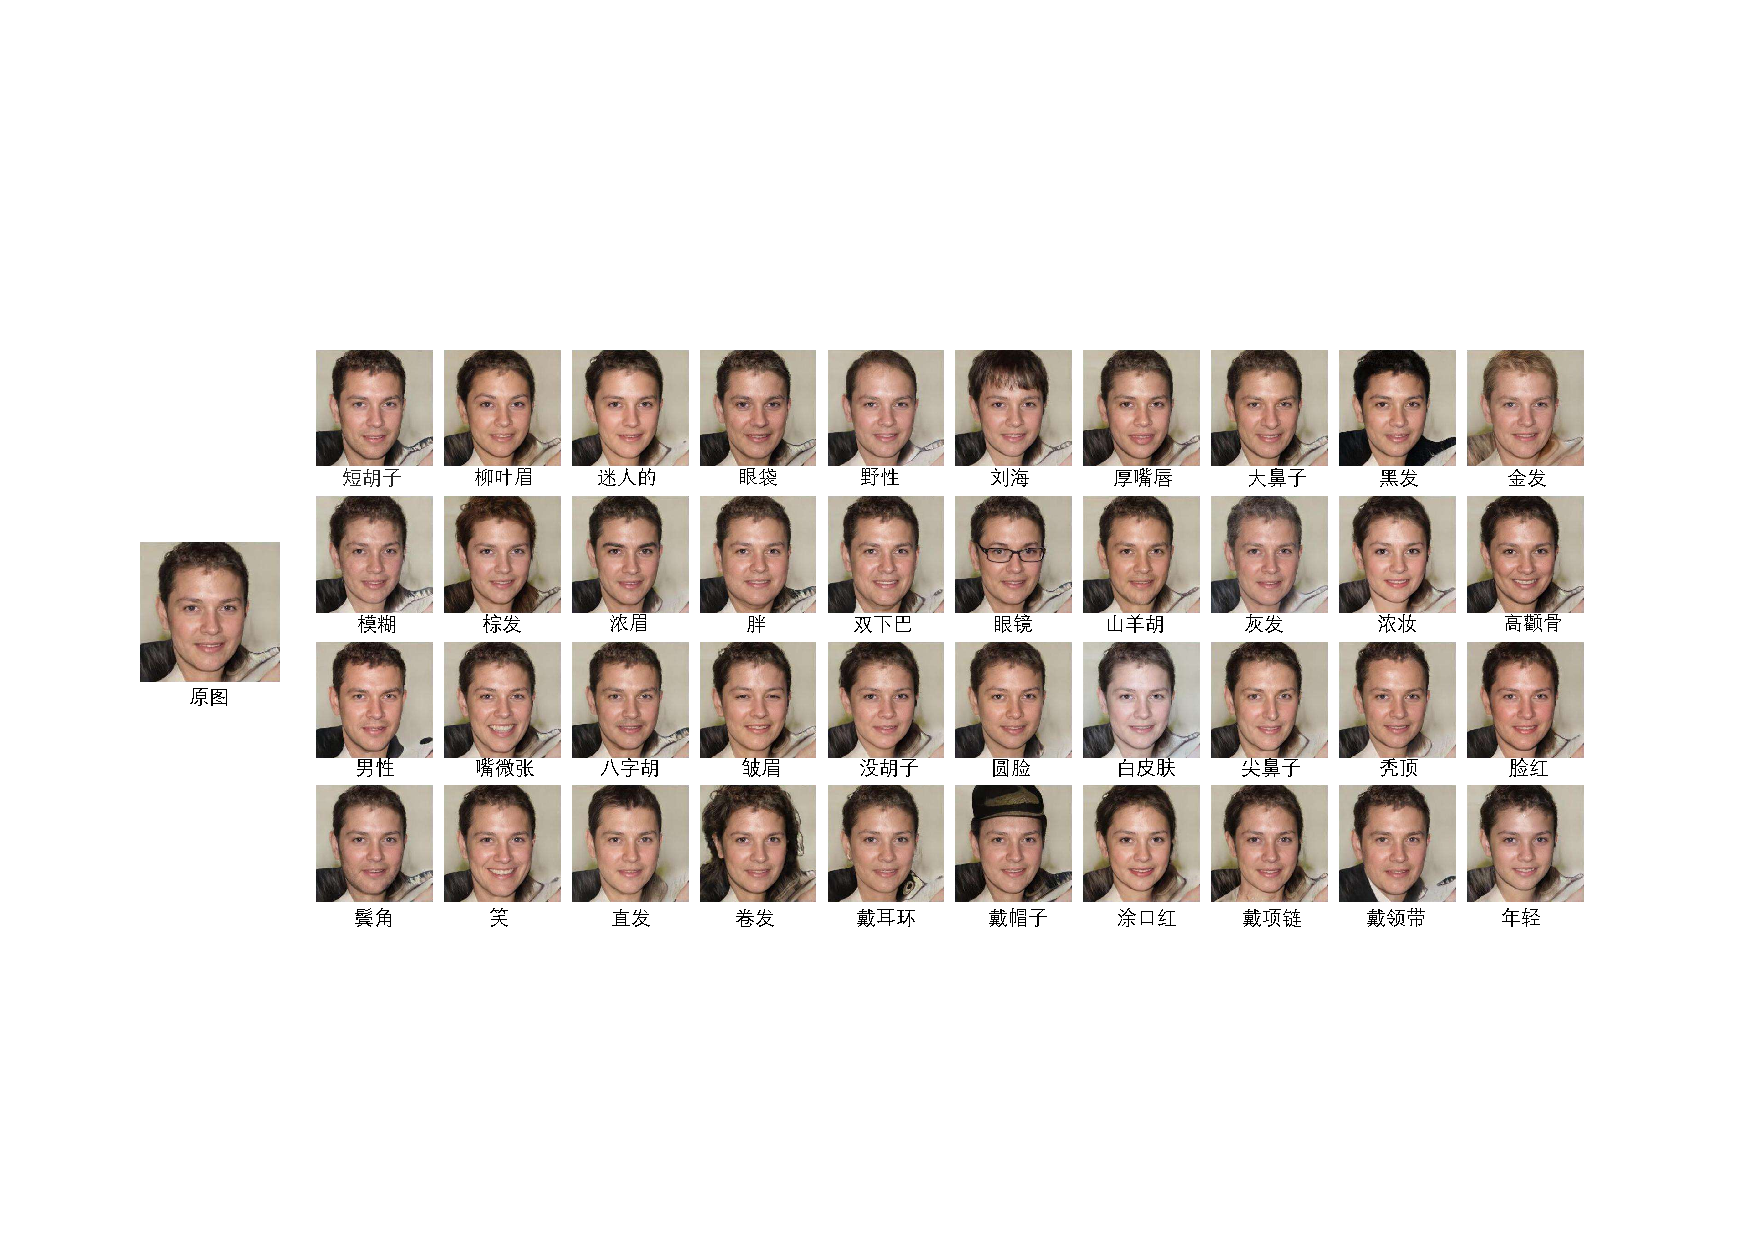
\includegraphics[width=0.9\linewidth]{figures/ACGAN/40Attributes.pdf}
    \end{center}
    \caption{40种属性的编辑}
    % \caption{Edited samples of all 40 attribute in CelebA dataset. The original image is generated under all attribute values equal to 0.5. For each attribute editing, we simply increase that attribute value to 1 and keep content values and other attribute values unchanged.}
    \label{fig:40Attributes}
\end{figure}

\subsubsection{$C$和$R$的分析}
我们将 $[0,1]$ 分成 20 个相等的间隔,并在 FFHQ 数据集上绘制属性 \textit{smiling} 得分的频率直方图。 如图~\ref{fig:quantization}(c)所示,sigmoid会将属性分类器$C$的输出推向接近0或1。$\mathcal{A}$训练的属性回归器也生成大部分预测值接近 到 0 或 1,如图~\ref{fig:quantization}(d)所示。相反,我们由 $\hat{\mathcal{A}}$ 训练的属性回归器 $R$ 产生了如图~\ref{fig:quantization}(e)所示的更合理的从 0 到 1 的连续值。 
% We divide $[0,1]$ into 20 equal intervals and plot frequency histogram of attribute \textit{smiling} score on FFHQ dataset. As shown in Fig.~\ref{fig:quantization}(c), sigmoid will push output of attribute classifier $C$ close to 0 or 1. Attribute regressor trained by $\mathcal{A}$ also generates most prediction values close to 0 or 1 as demonstrated in Fig.~\ref{fig:quantization}(d). On the contrary, our attribute regressor $R$ trained by $\hat{\mathcal{A}}$ produces more reasonable continuous values from 0 to 1 as in Fig.~\ref{fig:quantization}(e). We provide more analysis in the supplementary material.

\subsection{自然风景属性编辑相关实验}

\subsubsection{定性比较}
在 \cite{iclr2021} 之后,我们将我们的 ACGAN 与图像到图像方法 CycleGAN~\cite{cyclegan}、RelGAN~\cite{relgan} 和 DRIT++~\cite{drit++} 进行比较,如图~\ref{fig:sceneComparison}。 我们根据属性值将 Transient Attributes 数据集分为两部分:\textbf{A} 部分(属性值 $>$ 0.5)和 \textbf{B} 部分(属性值 $\leq$ 0.5)。 这些方法是通过从 \textbf{A} 部分到 \textbf{B} 部分的转换图像从头开始训练的,反之亦然。
如图~\ref{fig:sceneComparison}所示,与其他方法相比,我们的ACGAN准确地改变了原始图像的属性,这表明我们的模型在自然属性编辑方面表现良好。
% Following \cite{iclr2021}, we compare our ACGAN with image-to-image methods CycleGAN~\cite{CycleGAN2017}, RelGAN~\cite{relgan}, and DRIT++~\cite{drit++} in Fig.~\ref{fig:sceneComparison}. We split Transient Attributes dataset into two parts based on attribute value: \textbf{A} part (attribute value $>$ 0.5) and \textbf{B} part (attribute value $\leq$ 0.5). These methods are trained from scratch by translation image from \textbf{A} part to \textbf{B} part and vice versa.
% As shown in Fig.~\ref{fig:sceneComparison}, compared with other methods, our ACGAN accurately change the attributes of the original images, which suggests that our model performs well in natural attributes editing.

\begin{figure}[t]
    \begin{center}
         \includegraphics[width=0.5\textwidth]{figures/ACGAN/Scenecomparison.pdf}
    \end{center}
    \caption{自然场景单属性编辑对比}
    \label{fig:sceneComparison}
\end{figure}

由于自然图像的属性易于观察,我们对自然场景合成进行连续属性编辑。与人脸合成类似,ACGAN 在编辑自然场景属性(即“夜晚”、“云”、“雾”、“冬天”和“晴天”)方面也表现出卓越的性能。 我们在图~\ref{fig:scene}中展示了我们在自然场景下,每种属性在上图中从 0 增加到 1时的连续属性编辑结果。 受益于正交属性空间,ACGAN实现了自然场景中的准确属性编辑。
% Since the attributes of natural images are easy to observe, we conduct continuous attributes edits on Transient Attributes dataset. Similar to face synthesis, ACGAN also shows superior performance in editing natural scene attributes, i.e., "night", "cloud", "fog", "winter" and "sunny". We present our continuous attribute editing results under natural scene in Fig.\ref{fig:scene}. Benefiting from the orthogonal attribute space, ACGAN achieves accurate attribute editing in natural scenes with regards to image identity preservation.

\begin{figure}
    \begin{center}
         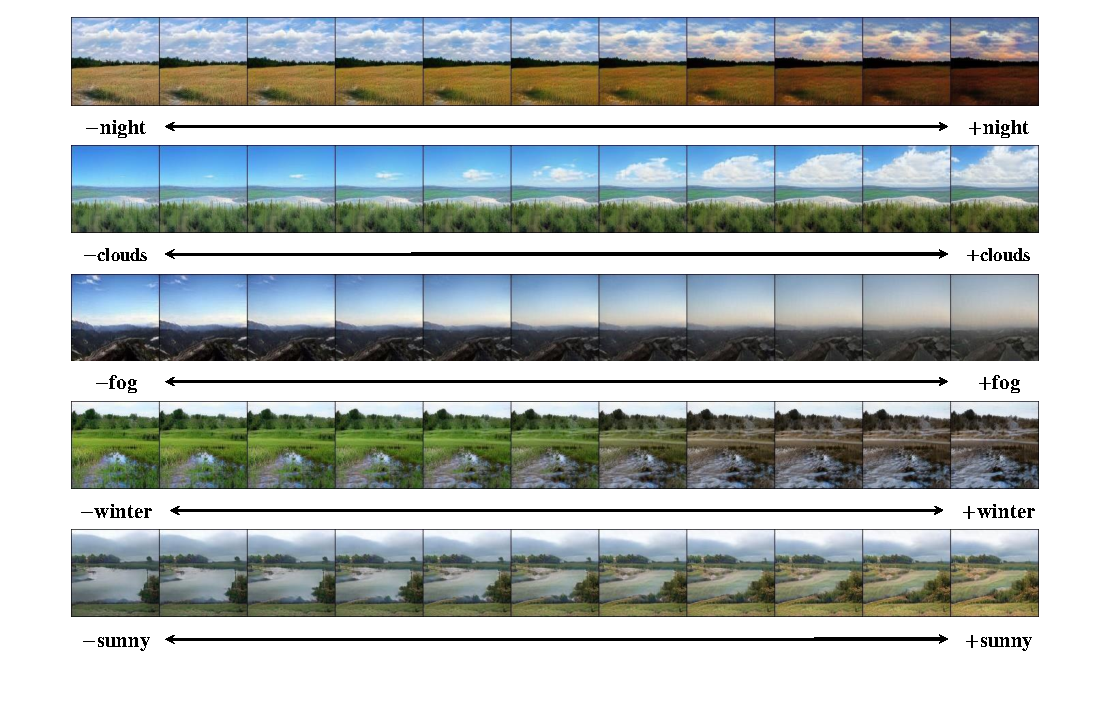
\includegraphics[width=0.85\linewidth]{figures/ACGAN/scene.pdf}
    \end{center}
    \caption{自然场景连续属性编辑}
    % \caption{Edited samples of 5 attributes in Transient Attributes dataset~\cite{scenedataset}. We demonstrate continuous changes in samples with each attribute increasing from 0 to 1 in the above picture.}
    \label{fig:scene}
\end{figure}

\subsubsection{定量比较}
为了定量评估我们的 ACGAN 在控制自然场景合成的属性方面,我们使用我们的 ACGAN 为每种属性生成 $5,000$ 的图像对 $(I_-,I_+)$。 $I_-$ 表示该属性为“关闭”或“负”,反之亦然。 我们在由属性回归器 $R$ 计算的 $(I_-,I_+)$ 之间定义属性增益(Attribute Gain)$AG$:
\begin{equation}
     AG = R(I_+)-R(I_-)。
\end{equation}
属性增益越大,该方法控制属性的能力越强。 为了与图像空间转换方法进行比较,我们使用 DRIT++ 和 RelGAN 生成额外的 $I_+$ 给定输入 $I_-$ 并计算它们之间的属性增益。从表~\ref{tb:attrbute_gain}展示的各个属性的增益对比中,可以看到我们的 ACGAN 的属性增益远高于其他方法,这证明我们的 ACGAN 对控制属性的能力最强。
% To quantitatively evaluate our ACGAN on controlling attributes for natural scene synthesis, we use our ACGAN to generate $5,000$ image pairs $(I_-,I_+)$ for each attribute. $I_-$ means this attribute is "off" or "negative" and vice versa. We define attribute gain between $(I_-,I_+)$ computed by attribute regressor $R$ : attribute gain=$R(I_+)-R(I_-)$. The larger the attribute gain, the stronger the method is in controlling attributes. To compare with image-space translation methods, we use DRIT++ and RelGAN to generate extra $I_+$ given input $I_-$ and compute attribute gain between them. The results are shown in Table~\ref{tb:attrbute_gain}. The attribute gain of our ACGAN is much higher than the other methods, which proves that our ACGAN has the strongest power over controlling attributes. 

\begin{table}[!t]
    \caption{属性增益对比}
    % \caption{The attribute gain of our ACGAN is much higher than the other methods, which proves that our ACGAN has the strongest power over controlling attributes.}
    \renewcommand\arraystretch{0.8}
    \begin{center}
    \begin{tabular}{lccccc}
    %{lC{3.4cm}C{3.3cm}C{2.8cm}}
    \toprule
    & 多云 & 雾 & 冬天 & 夜晚 & 晴天\\
    \midrule
    RelGAN & $0.1271$ & $0.1046$ & $0.1009$ & $0.1692$ & $0.1918$ \\
%   \hdashline
    \specialrule{0em}{1pt}{1pt}
    DRIT++ & $0.1183$ & $0.0177$ & $0.1496$ & $0.1055$ & $0.0736$ \\
%   \hdashline
    \specialrule{0em}{1pt}{1pt}
    \textbf{Ours} & $\textbf{0.3069}$ & $\textbf{0.2656}$ & $\textbf{0.5979}$ & $\textbf{0.2679}$ & $\textbf{0.3192}$ \\
    \toprule
    \end{tabular}
    \end{center}
    \label{tb:attrbute_gain}
\end{table}

\section{其他视觉效果展示}
本节我们将通过不同的实验设置,进一步展示ACGAN强大的图像属性编辑能力。

\subsection{人脸叠加属性编辑}
人脸叠加属性编辑指在一张图片上依次加入多种属性编辑。 如图~\ref{fig:multiAtt}所示,我们将属性变化+年龄、+白头发、+眼镜、+胡子(男性)或+化妆(女性)、+ 瘦
和+笑容依次加入到原始图像中。我们的方法可以在保持人物身份不变的前提下做出准确的属性编辑。


\begin{figure}[!t]
    \centering
    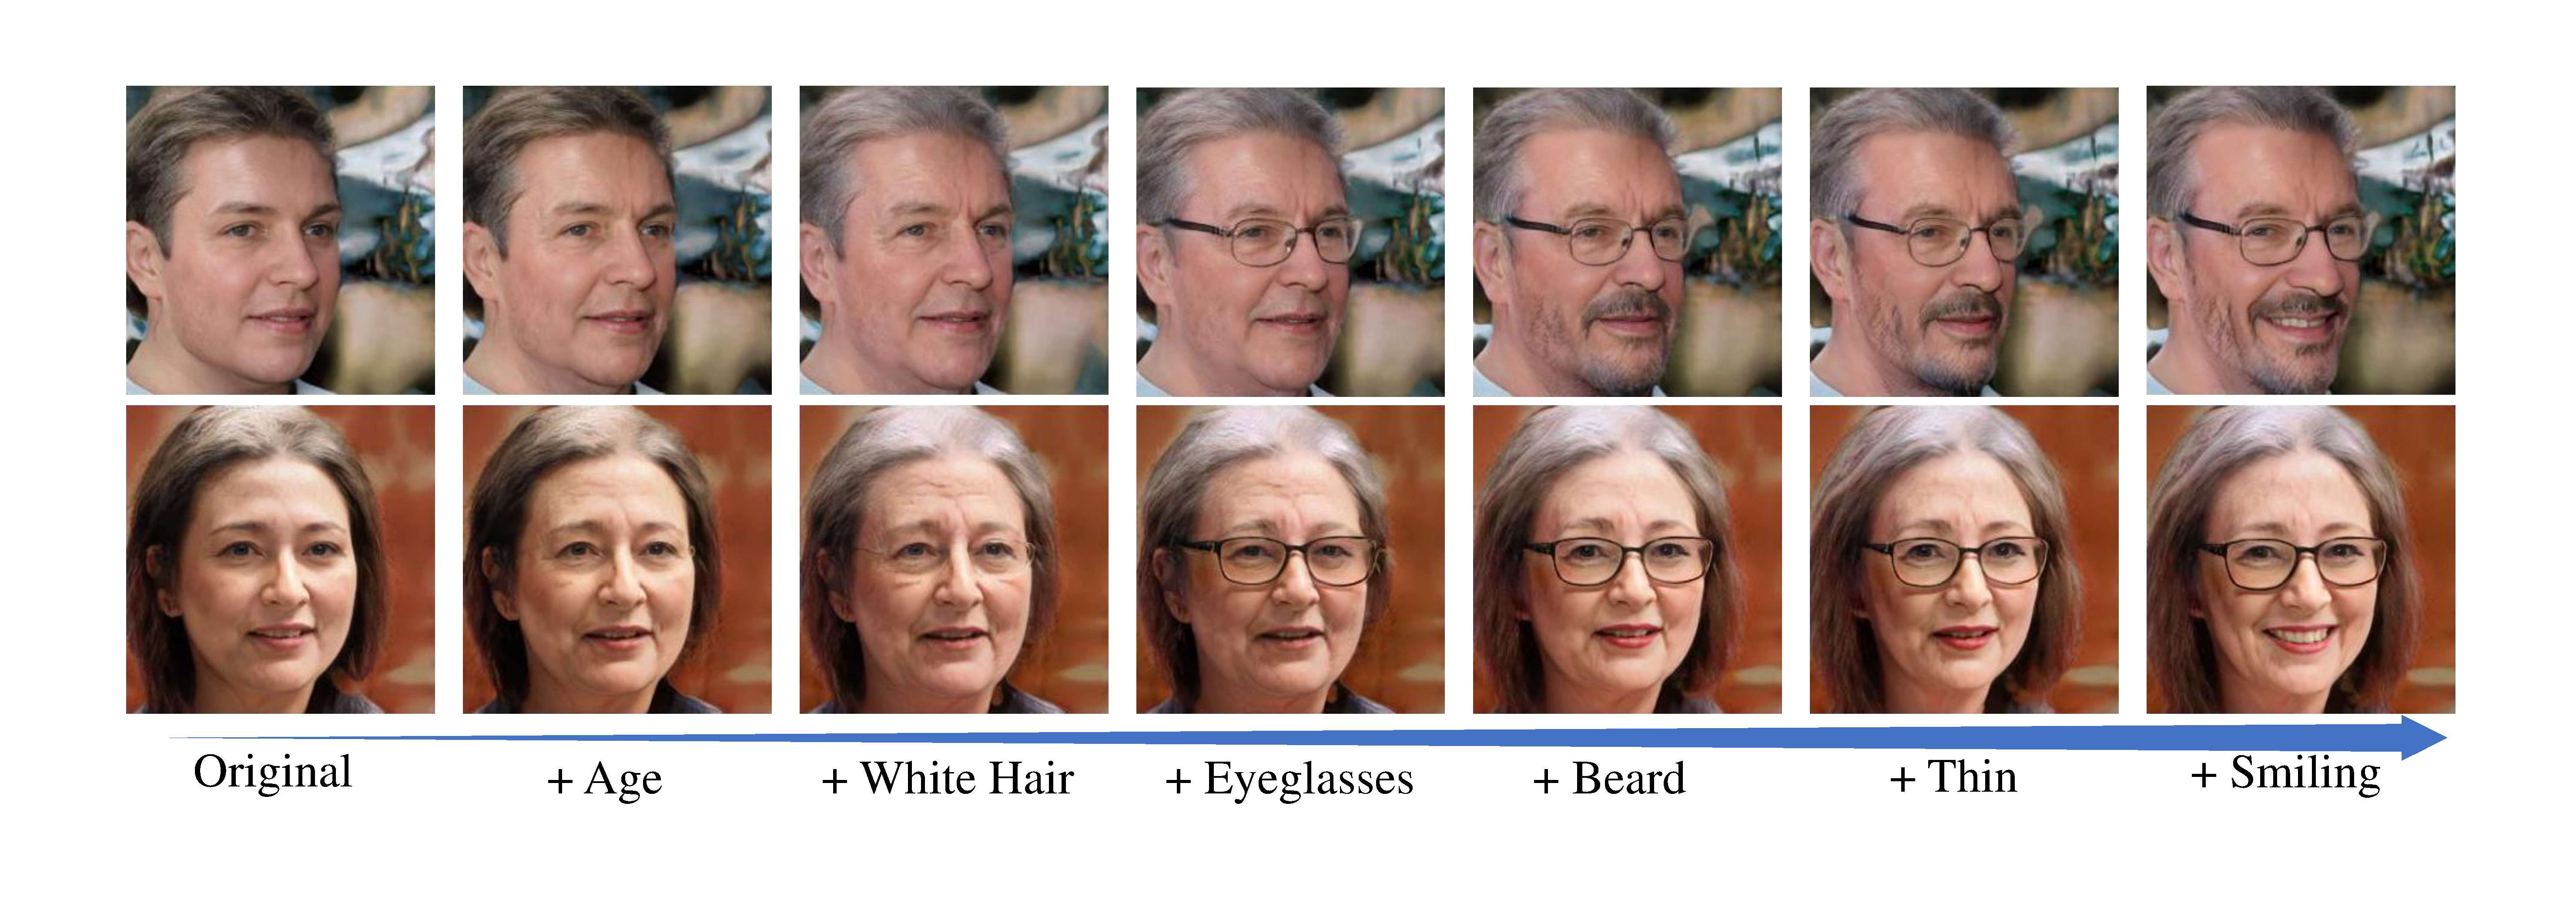
\includegraphics[width=0.8\textwidth]{figures/ACGAN/cover.pdf}
    % \caption{Accumulative attribute editing. We gradually enhance a certain attribute(age, white hair, etc.) from left to right in the portraits. Benefiting from disentanglement between attributes, the editing results are precise and smooth. Zoom in for better view.}
    \caption{人脸叠加属性编辑图}
    \label{fig:multiAtt}  
\end{figure}


我们进一步进行了增强和减弱属性年龄、眼镜、胡子、胖瘦和笑容的实验。实验过程中我们通过性别属性控制生成人物的性别,对于性别为女性的图像我们将胡子属性替换为化妆。 如图~\ref{fig:male}和图~\ref{fig:female}所示,我们的ACGAN可以对多个面部属性进行复杂的编辑。
% Here we show additional results of accumulatively manipulating multiple attributes on face images. The attributes \textit{Age}, \textit{White Hair}, \textit{Eyeglasses}, \textit{Beard}, \textit{Thin} and \textit{Smiling} are added accumulative to the original images. As shown in Fig.~\ref{fig:multiAtt}, our method can generate accurate attribute editing with excellent identity consistency and realistic textures. 
% We further conduct experiments on adding and removing the attributes \textit{Age}, \textit{Eyeglasses}, \textit{Beard}, \textit{Chubby} and \textit{Smiling} in turn to more images with \textit{Male} attribute. For the image with \textit{Female} attribute, we replace the \textit{Beard} attribute with the \textit{Makeup} attribute. As shown in Fig.~\ref{fig:male} and Fig.~\ref{fig:female}, our ACGAN is qualified to complex manipulation on multiple facial attributes.

\begin{figure}[!t]
     \begin{center}
          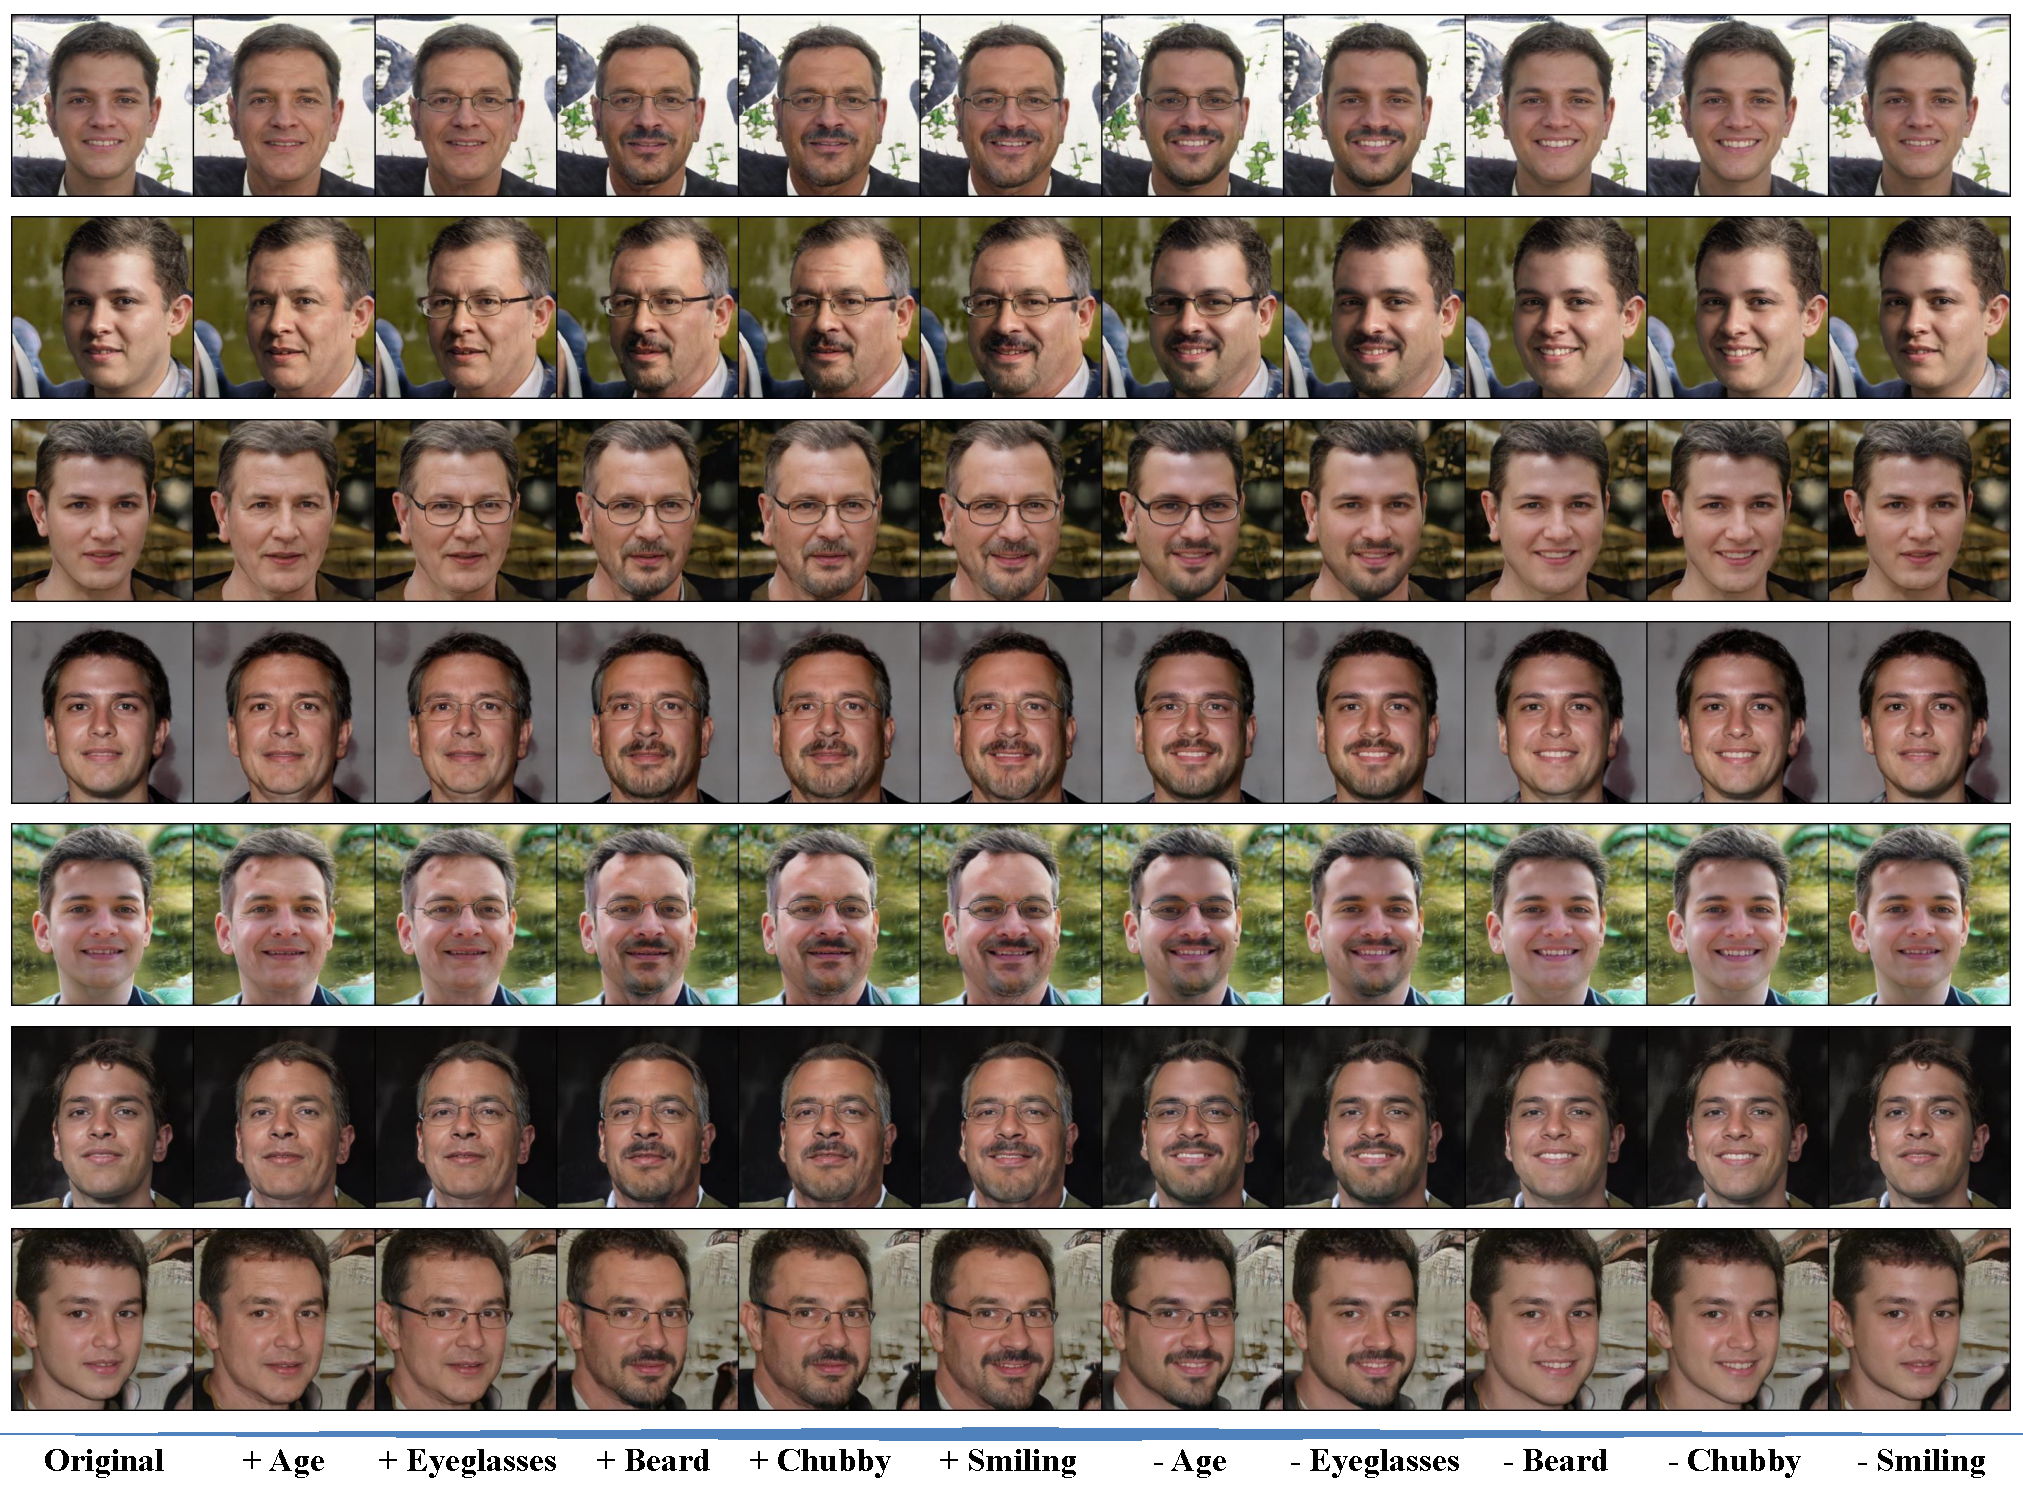
\includegraphics[width=0.8\textwidth]{figures/ACGAN//male.pdf}
     \end{center}
     \caption{男性人脸叠加属性编辑图}
     \label{fig:male}
\end{figure}

\begin{figure}[!t]
     \begin{center}
          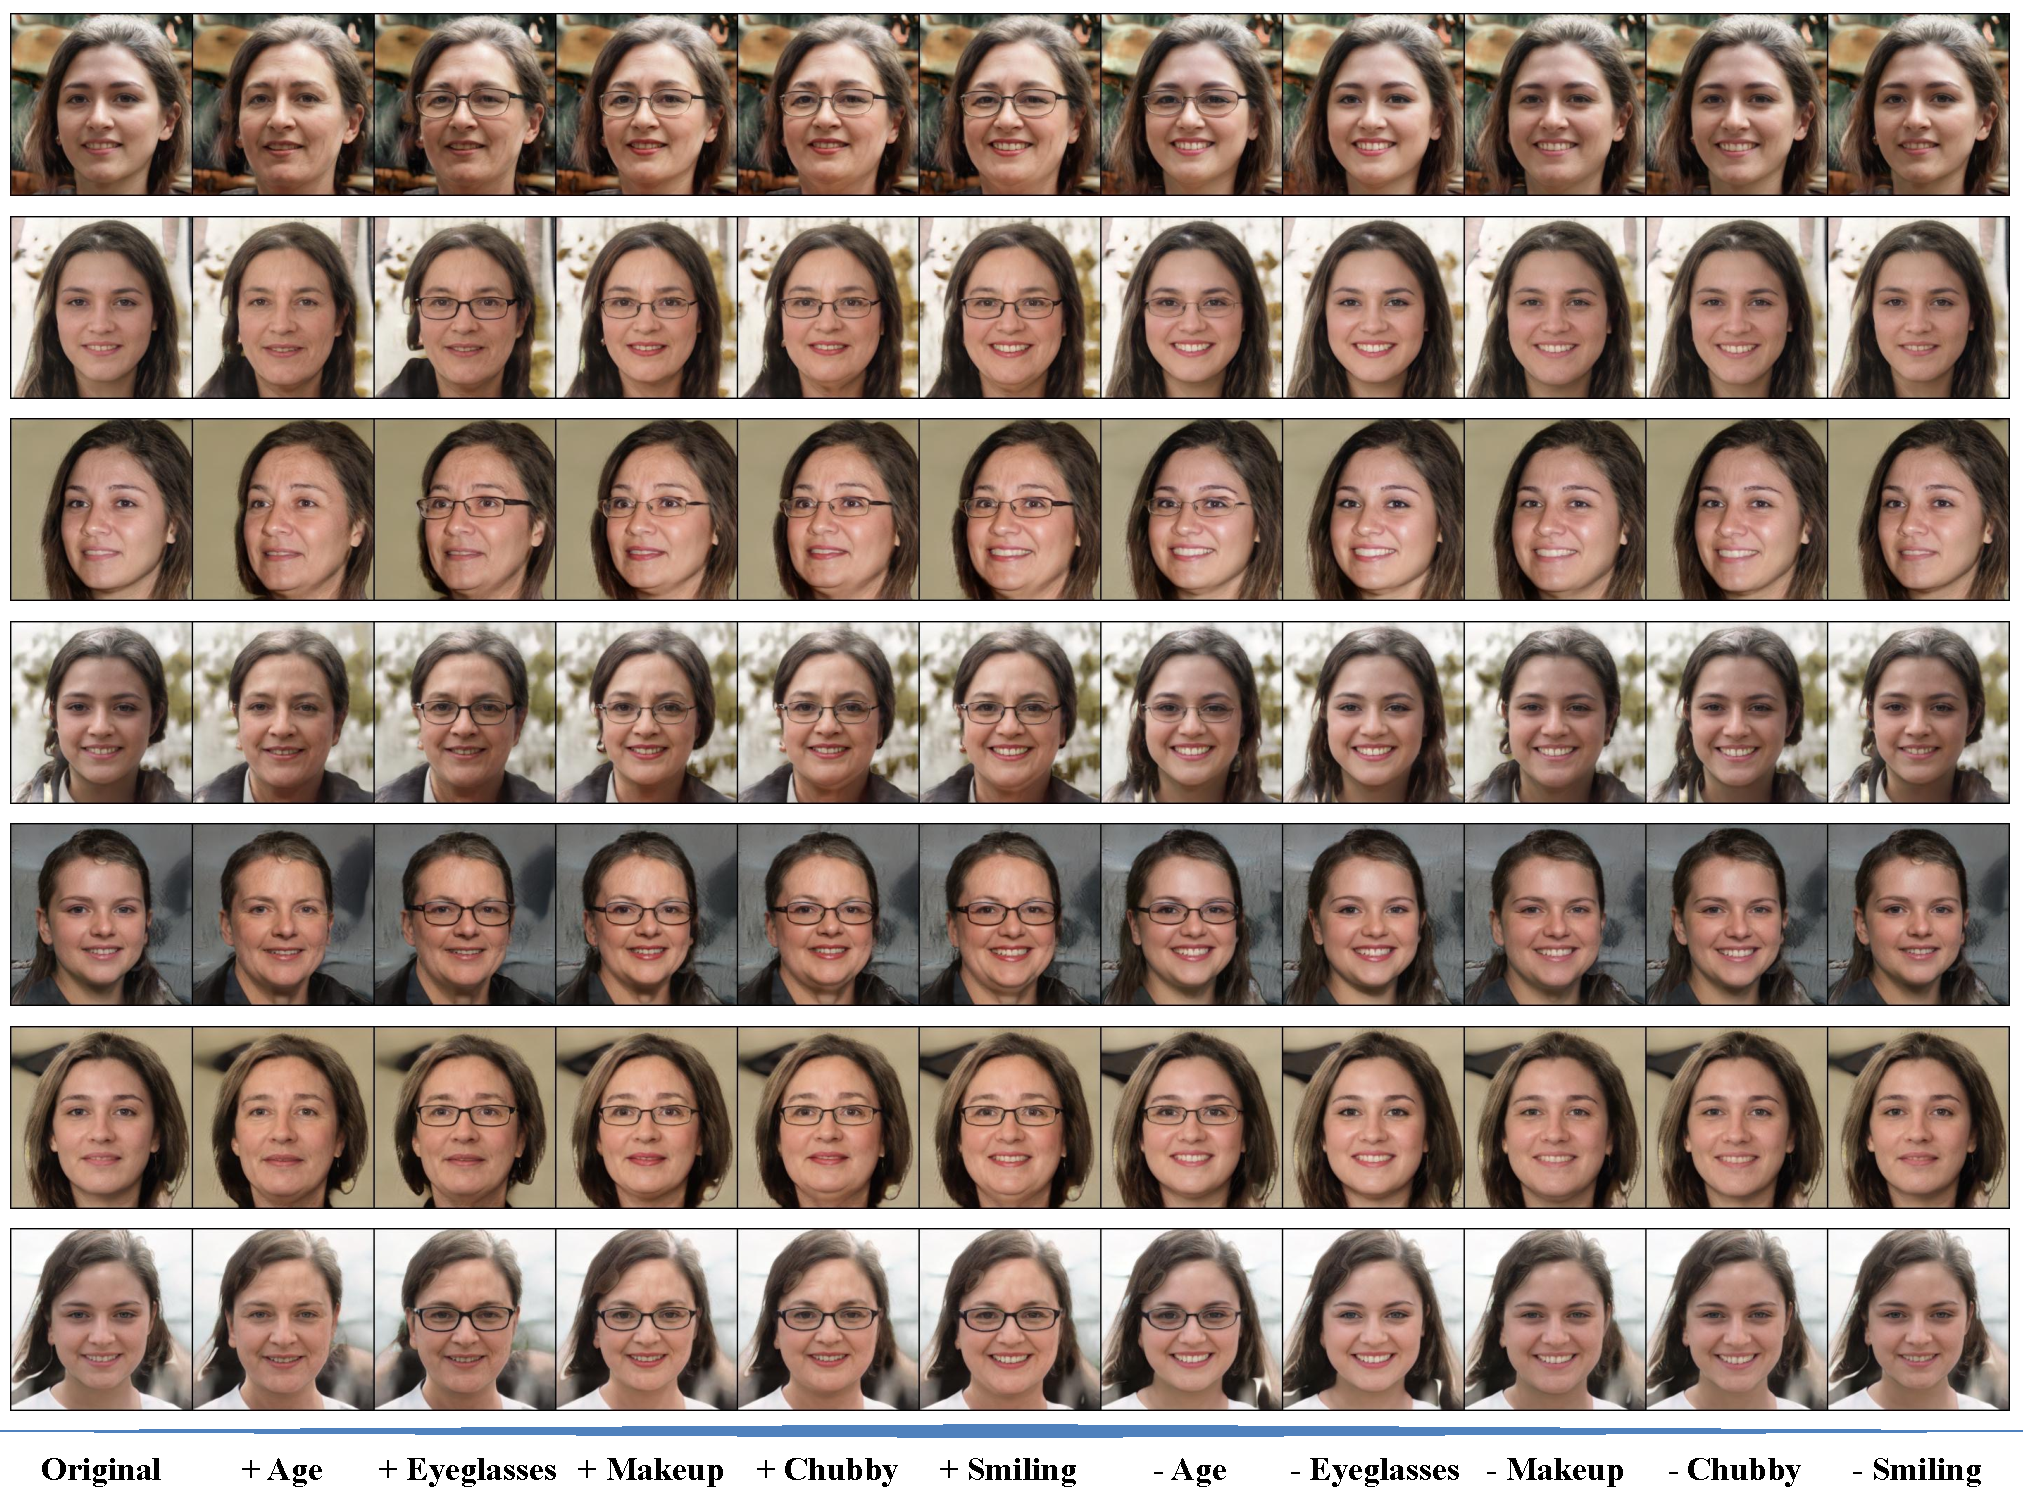
\includegraphics[width=0.8\textwidth]{figures/ACGAN//female.pdf}
     \end{center}
     \caption{女性人脸叠加属性编辑图}
     \label{fig:female}
\end{figure}


\subsection{自然场景复合属性编辑}
我们在图~\ref{fig:sceneMulti} 中展示了ACGAN对自然场景图像进行复合属性(两种属性)编辑的结果。图~\ref{fig:sceneMulti}(a)显示了云和雾的编辑结果,位于(a)左上角的图片既没有雾也没有云,(a)下边的图片包含更多的云和较少的雾,(a)右边的图片往往会产生更多的雾和较少的云;(a)右下角的图片则同时包含较多云和雾。图~\ref{fig:sceneMulti}(b)和(c)遵循类似的规律。就属性解耦来说,三种属性组合:云与雾、云与冬天(季节变化)、云与晴天(天气变化),均实现了肉眼可见的属性解耦。 该实验进一步证明了我们的方法在解耦自然场景属性方面的优越性。
% We present additional results of multiple attributes editing on natural scene images in Fig.~\ref{fig:sceneMulti}. The generated images generated by our method are manipulated on two attributes simultaneously. Fig.~\ref{fig:sceneMulti}(a) shows the results of editing \textit{Clouds} and \textit{Fog}, the top left picture shows neither fog nor clouds, the downwards pictures tend to generate more clouds and less fog, the rightward pictures tend to generate more fog and less clouds; the bottom right picture contains both clouds and fog. Fig.~\ref{fig:sceneMulti}(b) and Fig.~\ref{fig:sceneMulti}(c) show similar performance in disentangling \textit{Clouds} with \textit{Winter} and \textit{Sunny}. This experiment demonstrates the advanced performance of our method in disentangling natural scene attributes. 

\begin{figure}[!ht]
	\begin{center}
		 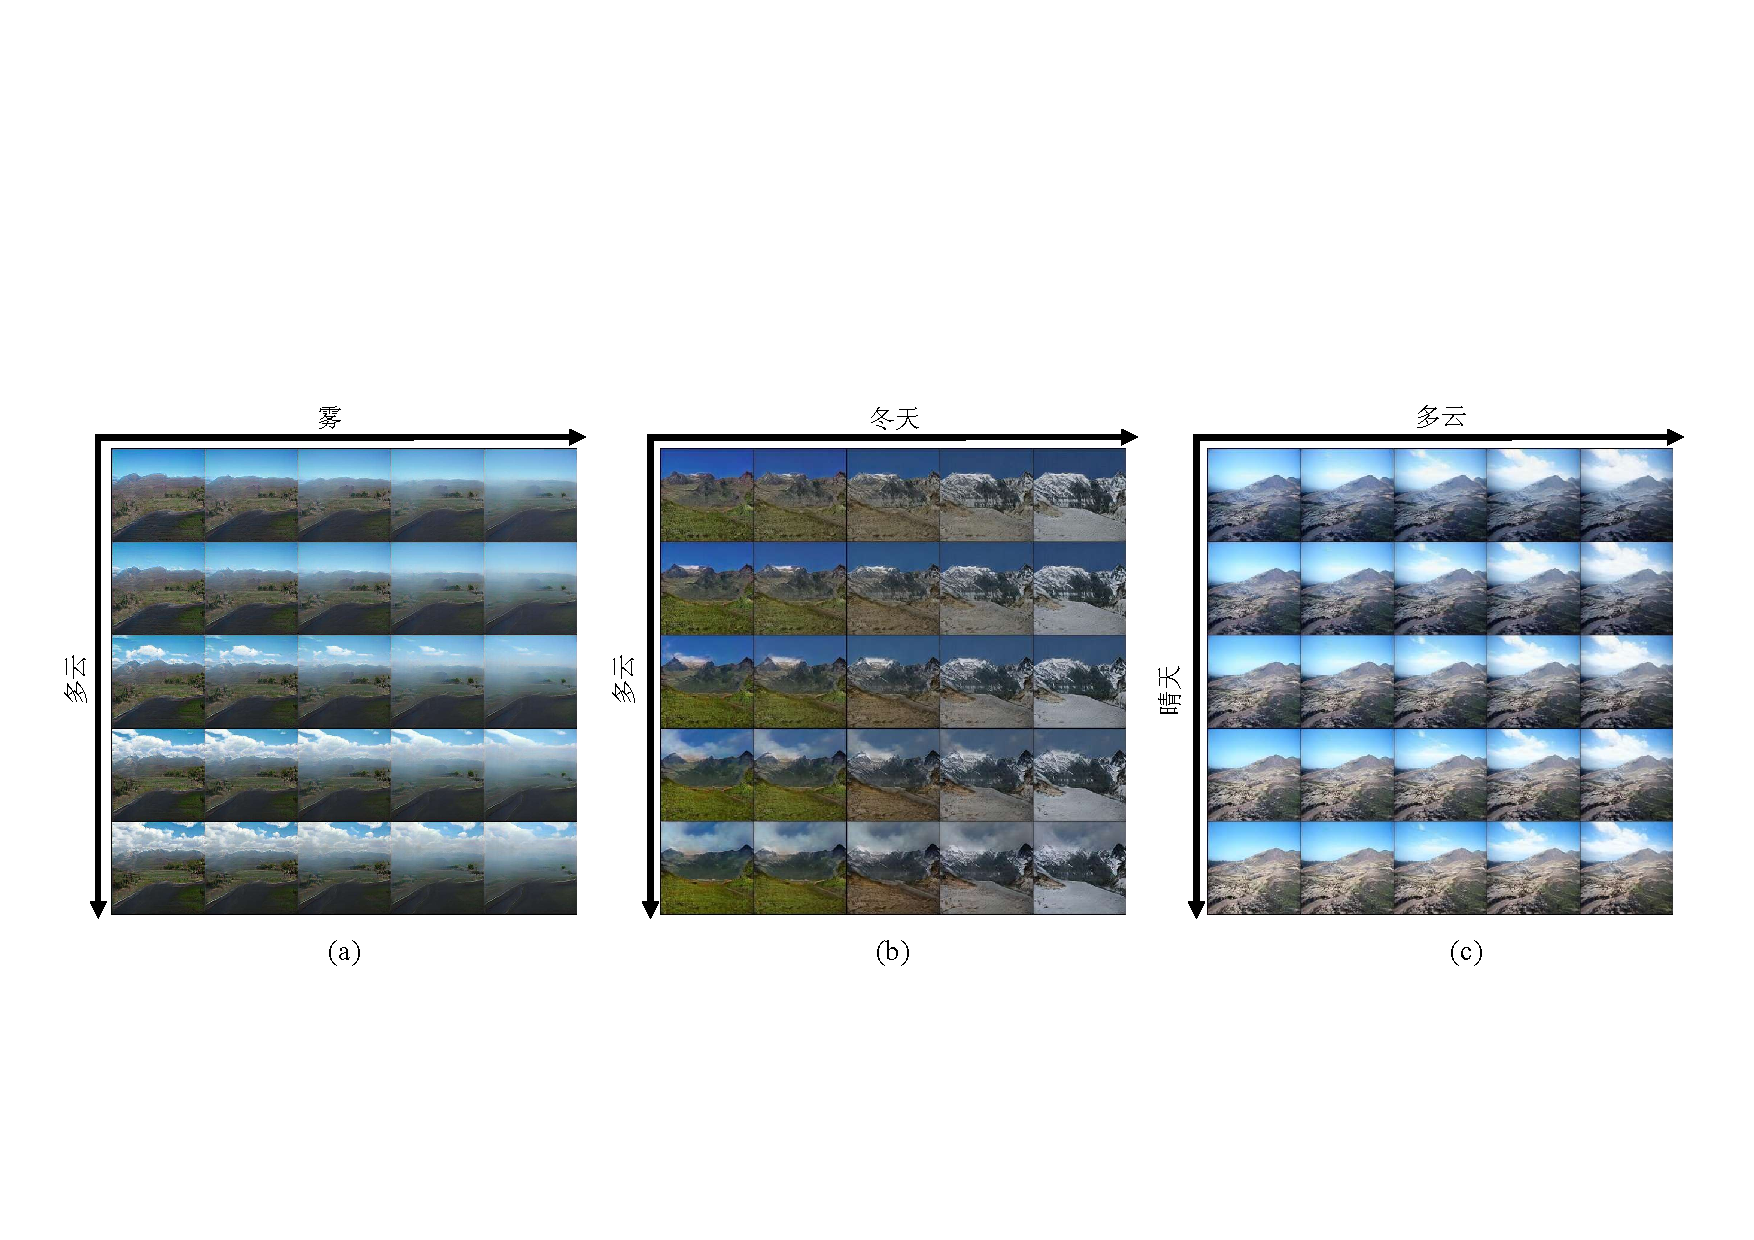
\includegraphics[width=0.8\textwidth]{figures/ACGAN/sceneMulti.pdf}
	\end{center}
	\caption{自然场景复合属性编辑图}
	\label{fig:sceneMulti}
\end{figure}

\section{本章总结}
在这项工作中,为了实现语义解耦的图像编辑,我们提出了一种输入属性与生成图像属性一致的生成式对抗网络ACGAN。 为了在理论上保证每种属性方向与其他方向解耦,我们将属性空间与内容空间隔离,将属性空间投影到正交空间,并提出了属性一致损失来约束输入属性与生成图像属性的属性一致性。为了将我们的方法扩展到所有带有属性标注的数据集,我们进一步提出了一种属性量化策略,将二进制属性标签量化为连续值。 实验证明我们的方法可以在保持图片身份信息不变的前提下,同时且连续地编辑多种属性。
% In this work, we propose a semantic controllable GAN for image attribute editing. To better disentangle each attribute direction from other directions, we isolate an attribute space from the latent space and project it to the orthogonal space. An attribute-consistent loss is proposed to constrain the continuous attribute consistency. To extend our approach to all the attribute datasets, we further propose an attribute quantification strategy to quantify binary attribute labels to continuous values. Experiments prove our method can simultaneously and continuously edit multiple attributes with high fidelity and semantic disentanglement. 

虽然我们提出的 ACGAN 与其他最先进的方法相比实现了更佳的性能,但仍存在一些局限性。 例如,属性的相似性(如灰色头发和苍白皮肤具有相似的颜色)可能导致属性难以完全解耦。 此外,真实图像编辑取决于 GAN 逆映射(GAN inversion)的结果,这通常需要复杂的 GAN 架构, 而我们采用的基本模型 StyleGAN2 仍然需要大量的时间进行训练。 未来,我们将探索更高效的回归器和 GAN 架构。
% While our proposed ACGAN achieves superior performance compared to other state-of-the-arts, there are several limitations. For instance, similar attributes may lead to regression errors. For example, Gray Hair and Pale Skin have similar colors, which may cause these attributes hard to disentangle. Besides, real image edits depend on the result of GAN inversion, which most often requires complex GAN architecture. Our used StyleGAN2 still takes huge time consumption. In the future, we would explore more efficient regressor and GAN architecture.
\clearpage{\pagestyle{empty}\cleardoublepage}
\chapter{基于生成式对抗网络的多模态图像转换}

多模态图像转换任务可以看作一类特殊的图像转换任务。近些年来,在研究人员的持续努力下,图像转换取得了很大进展,但现有的工作难以对多个输入之间的相关性进行建模,因此多模态图像转换仍非常具有挑战性。在本文中,我们提出了一种新颖的联合注意力GAN (Joint Attention Generative Adversarial Networks,JAGAN) 框架,通过可用的多模态图像生成缺失的模态图像。为了更有效地提取与目标模态一致(相关)的多模态表示,我们使用自表示网络来驱动我们提出的联合注意力机制。JAGAN提取的多模态特征可以与目标模态保持通道级的一致性,极大地提高了图像转换性能。通过与现有方法在多模态图像转换任务上定量和定性比较,证明了我们方法的能够生成更精准的缺失模态图像。

\section{引言}

图像处理、计算机视觉和计算机图形学等越来越多的应用开始依赖于多模态图像,如在精准医学领域,脑部核磁共振可以得到T1、T1Gd、T2和T2-FLAIR四种模态~\cite{drevelegas2011imaging},医生希望尽可能结合完整的多模态医学图像来做出更精确的诊断,但往往受限于实际条件(受限的医疗条件、扫描时间不足以及成本/支出/资源等限制),在多模态数据获取过程中可能出现系统误差,甚至部分模态的缺失~\cite{tanenbaum2017synthetic}等情况。这些不可用的模态图像可能会导致医生决策出现偏差。

由于我们在实践中经常会遇到低质量甚至缺失的模态图像,如何利用已有的、完整的模态图像数据对不可用的模态进行填补,已成为计算机视觉和图像处理中的一个重要研究课题。除了可用的图像数据外,医生还可以使用填补的缺失模态数据辅助决策。

对多模态图像数据中缺失的模态进行填补可以看作是一个图像转换问题。图像转换指将图像从一个图像域转换到另一个图像域,类似的任务包括风格转移、分割、去模糊、超分辨率等。不同图像域指的是光照条件、面部表情、传感器等之间的各种成像差异。研究人员为研究有效的图像转换算法投入了大量精力,并在基于生成对抗网络的方法上取得了重大进展,例如Pix2Pix~\cite{pix2pix}、CycleGAN~\cite{cyclegan}和StarGAN~\cite{stargan}等。然而,这些方法仅适用于单一模态输入,在模型输入与网络设计上并未考虑多模态场景下其他可用模态中包含的有效信息。 CollaGAN~\cite{collagan} 是少数为多模态设计的图像转换模型之一,Dongwook Lee等人针对多模态场景,在CycleGAN的基础上提出多重循环一致性损失,从而实现了从任意多模态输入生成目标模态图像的功能。

CollaGAN的缺点在于没有针对跨模态一致性和模态间互补性进行约束,这使得其不能充分利用输入模型的信息。为了有效地提取目标模态(缺失模态)的多模态表示,充分利用模态间一致性和互补性,我们提出基于联合注意力机制机制的生成对抗网络,用于多模态图像转换。我们从一致性和互补性两个方面约束JAGAN的训练:
对于一致性,我们引入自表示网络,结合我们提出的模态内注意力机制,监督模型在训练过程中从输入模态中提取与目标模态一致的特征;
对于互补性,我们设计了模态间注意力:根据模态间互补性以输入模态的信息补充生成目标模态所需要的信息。模态间注意力需要模态特征之间的兼容性,而这由我们的模态内注意力机制通过一致性约束提供。我们将提出的模态内注意力与模态间注意力机制结合,提出用于多模态图像转换的联合注意力生成式对抗网络。

% 我们提出的框架由转换网络和自表示网络组成。

我们提出基于联合注意力机制机制的生成对抗网络贡献如下:

\begin{enumerate}
\item 我们提出模态间注意力,用于模态间互补性用输入模态的信息补充生成目标模态所需要的信息。
\item 我们引入自表示网络来指导训练期间的生成模型,这提供了模态补充模块所需的特征兼容性,并在特征提取阶段过滤掉无关信息。
\item 通过与现有方法在多模态图像转换任务的定量和定性比较,证明了我们方法的能够生成更精确和逼真的结果。
\end{enumerate}


\section{联合注意力生成式对抗网络}
为了尽可能地提取与目标模态一致的多模态表示,并充分利用模态间互补性,从而提高缺失模态图像的生成质量,我们提出了联合注意力机制,并与自监督学习相结合,提出了一种新的多模态图像转换框架JAGAN。我们提出的JAGAN可以灵活地从可用模态中生成任何缺失的模态。

\subsection{概述}

受\cite{zhang2020deep}的启发,我们为多模态图像转换任务提出了模态间互补性和跨模态一致性:
\begin{itemize}
    \item 跨模态一致性:只有与目标模态一致(相关)的特征才能被提取出来,无关的信息的应该被过滤掉。
    \item 模态间互补性:对于多模态任务,大多数模态包含其他模态不包含的信息。可以利用这种性质来估算更好的缺失模态。
\end{itemize}

现有的基于生成式对抗网络的图像转换方法取得了很大进展,但这些方法忽略了可用多模态图像之间的一致性与互补性。对于一致性,我们使用自表示网络,结合我们提出的模态内注意力机制,监督模型在训练过程中从输入模态中提取与目标模态一致的特征。对于互补性,由于目前多模态图像转换任务缺乏大规模数据集,这使得网络很难自动学得如何最大程度地利用模态间互补性。为了解决这个问题,我们提出了模态间注意力,用从其他输入模态中提取的特征来补充生成目标特征所需的特征。

如图~\ref{f1}所示,我们的JAGAN由自表示网络和转换网络组成,转换网络由GANs实现。出于模态间的互补性,模态间注意力在特征融合之前每个输入模态补充来自其他模态信息。考虑到自编码器强大的自表示能力,我们在此采用自编码器网络作为自表示网络来引导模态内注意力的训练,约束生成器在特征提取阶段只提取与目标模态一致(相关)的特征,这进一步为模态间注意力提供必要的模态特征兼容性。

\begin{figure}
    \centering
    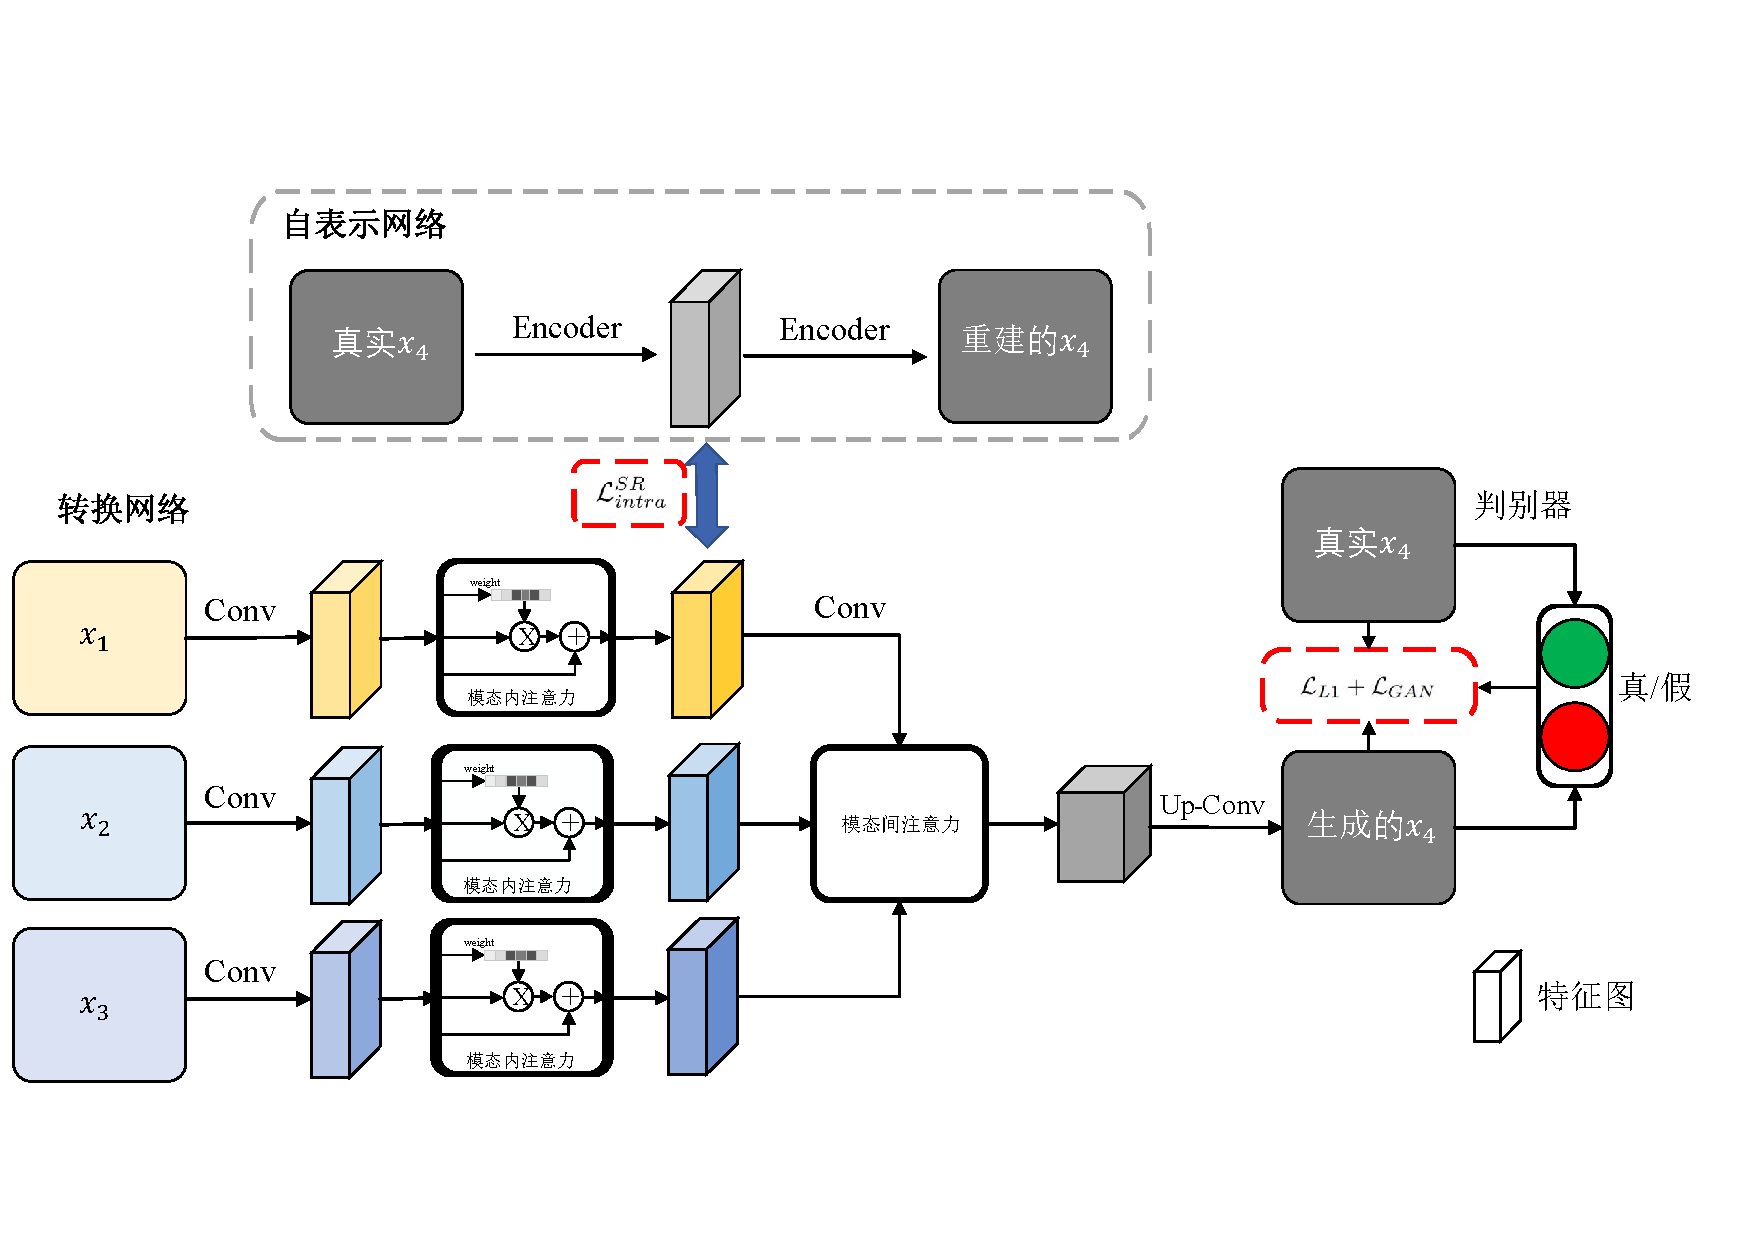
\includegraphics[width=1\columnwidth]{figures/JAGAN/framework.pdf}
    \caption[aaa]{JAGAN框架图。来自模态$\{m_1, m_2, m_3\}$的输入图像$\{x_1, x_2, x_3\}$分别被送入转换网络对应的分支,来生成目标模态$m_4$的图像$x_4$。我们结合模态内注意力和模态间注意力提取生成模态目标所需特征,模态内注意力受自表示网络监督。}
    \label{f1}
\end{figure}

不失一般性,为了便于表示,我们假设数据集中存在四种模态 $\{m_1, m_2, m_3, m_4\}$。对于转换网络,我们假设模态 $\{m_1, m_2, m_3\}$ 中的输入图像 $\{x_1, x_2, x_3\}$ 被转换为目标模态 $m_4$ 中的目标图像 $x_4$。

\subsection{模态内注意力与自监督学习}

正如我们前面提到的,我们引入了一个自编码器来驱动转换网络$\mathcal{T}$的训练,它由一个带有多分支编码器和单个分支解码器的生成器$\mathcal{G}$和判别器$\mathcal{D}$组成,自表示网络$SR$由自编码器实现。

$SR$ 以通道为粒度驱动 $\mathcal{T}$ 进行训练:
\begin{align}
	\mathcal{L}_{SR} = \sum_{k=1}^n \|f^{SR}_{x_i}- E^{SR}(x_{m_4})\|_2
\end{align}

其中 $E^{SR}(x_{m_4}$表示自表示网络编码器的输出,$f_{x_k}=E_k(x_k)$,$E_k(\cdot)$ 表示生成器$G$第$k$个编码分支$E_k$的输出。

\subsection{模态间注意力}

特征图中的每个通道都可以看作是深度神经网络从输入中提取的某种模式。对于任意通道而言,每个输入模态中包含的信息是不同的。我们仍以医学图像为例,如果第k个通道是关于肿瘤的纹理特征,显然T1Gd包含最丰富和最有价值的信息;如果该通道是关于脑脊液的,那么T2是最重要的模态。一个自然的想法是将T1Gd中的肿瘤相关信息添加到T2模态中,并将T2中的脑脊液相关信息添加到T1Gd模态中。这实际上就是在利用模态间的互补性。

请注意,在向其他模态补充信息之前,对于给定的通道或模式,我们需要知道哪种模态包含最丰富的信息,或者我们需要更多关注哪种模态。受注意力机制~\cite{seq2seq,attentionallyouneed,nonlocal,sagan}的启发,我们提出了一种如图~\ref{f2}所示的模态注意力机制,来计算跨模态的通道权重(表示为 $\mathcal{A}$)。

\begin{figure}
	\centering
	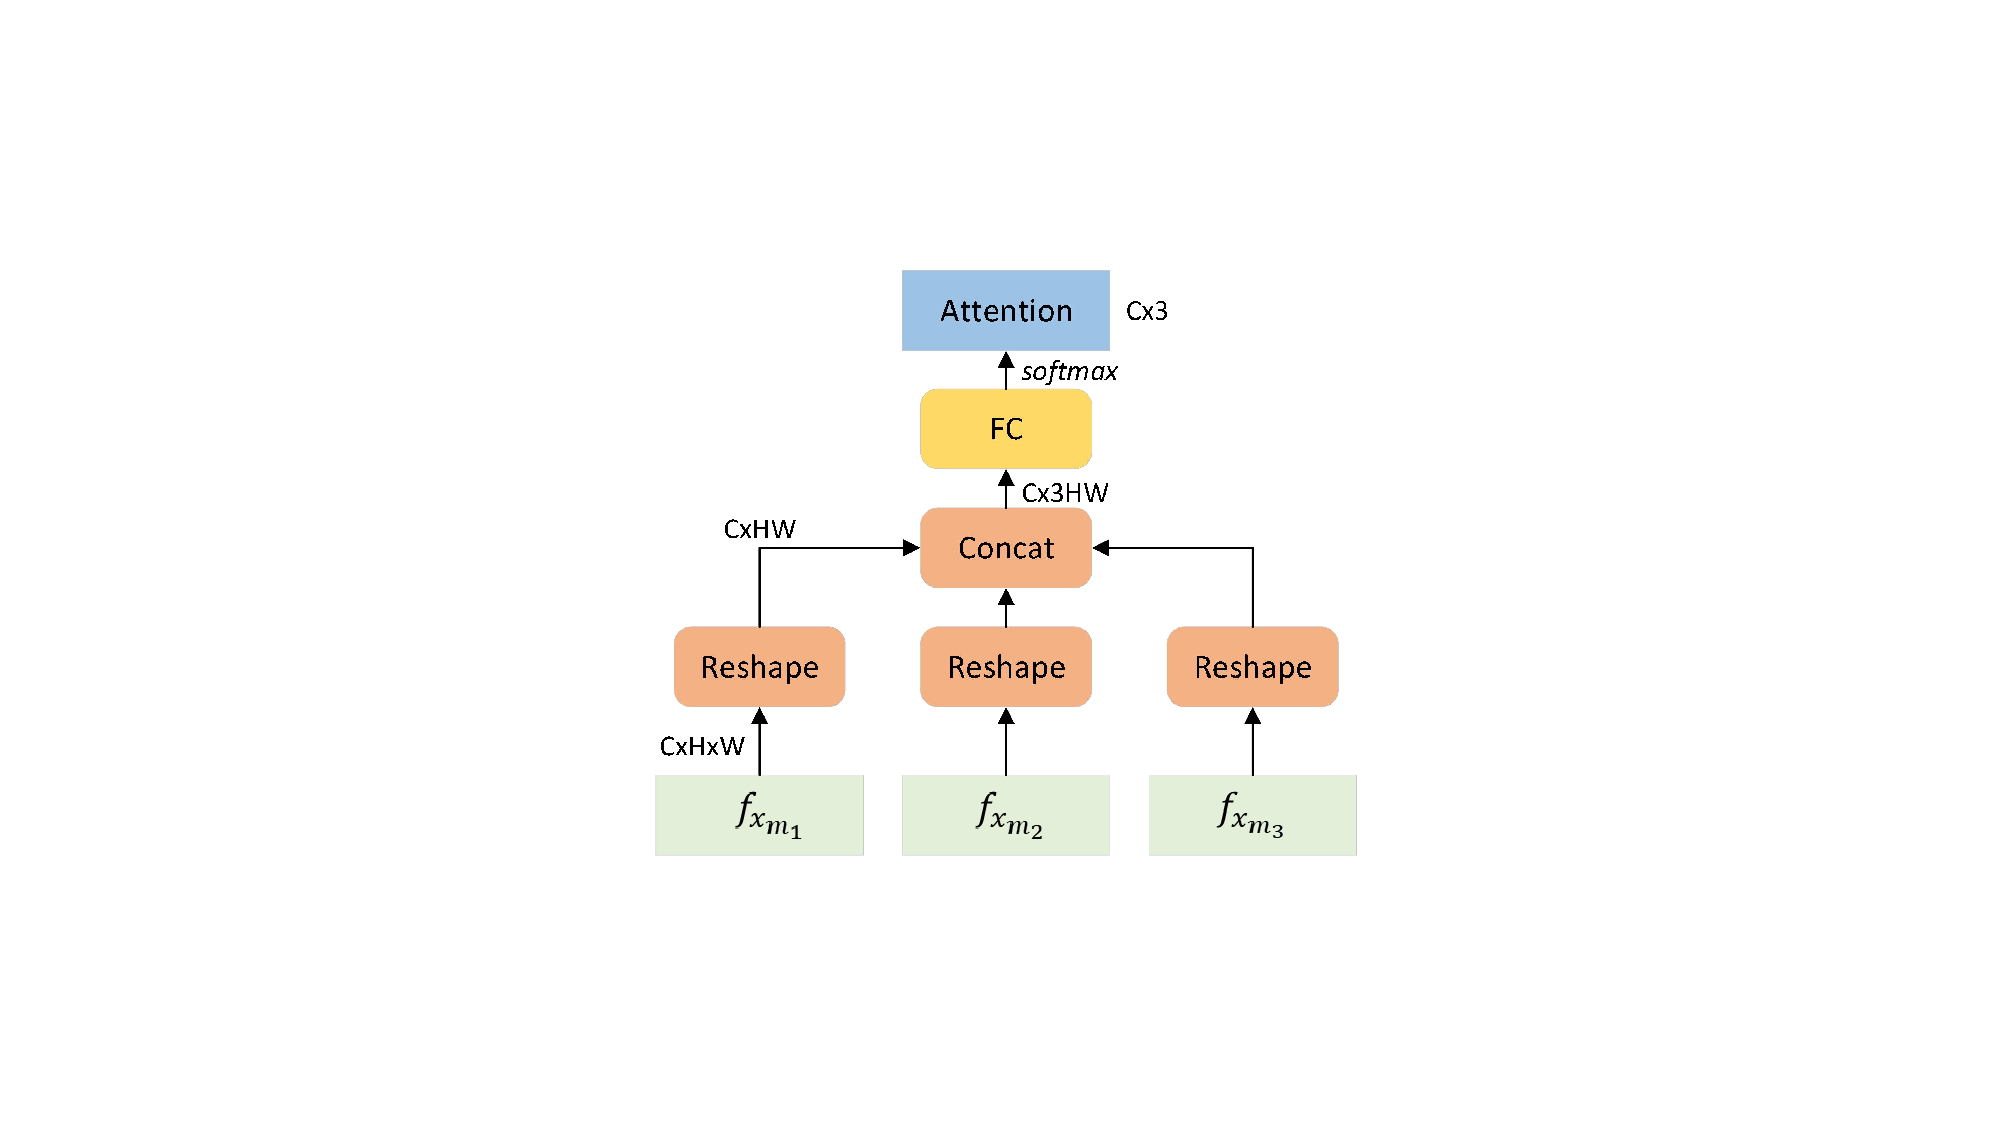
\includegraphics[width=0.8\columnwidth]{figures/JAGAN/20201109InterAttention_function_AV1_0.pdf}
	\caption[]{模态间注意力机制的注意力矩阵计算过程. FC表示公式\ref{e1}中定义的两层全连接层。}
	\label{f2}
\end{figure}

\begin{align}
	\mathcal{A} = S_2(\sigma((\delta([f_{x_1}, f_{x_2}, f_{x_3}]W_1))W_2))\
	\label{e1}
\end{align}

其中 $f_{x_k}=E_k(x_k)$,$E_k(\cdot)$ 表示生成器$G$第$k$个编码分支$E_k$的输出,$[\cdot,\cdot]$ 表示张量reshape(将张量从CxHxW展平至CxHW)和串联。 $W_1$和$W_2$是两个全连接层,如图~\ref{f2}。$\delta$和$\sigma$ 分别是ReLU\cite{nair2010rectified}和Sigmoid 函数。 $S_2$是 对$\mathcal{A}$ 每一行进行softmax运算的函数。从结果上来看,元素$\mathcal{A}_{i,j}$第$i$个模态对第$j$个的模态的注意力,换句话说,是用第$j$个的模态向第$i$个模态补充信息时的权重。

如图\ref{f3}所示,我们使用$\mathcal{A}$将其他模态的信息补充到每个输入模态中。通过这种方式,我们可以获得生成$i$-th模态所需的的互补特征$f_{x_i}^{comp}$:
\begin{gather}
	f_{x_i}^{comp} = \gamma * f_{x_i} +
	(1-\gamma) * \sum_{k=1}^n (f_{x_k} * \mathcal{A}_{k})\
\end{gather}
其中$*$表示向量和特征图之间的通道乘法,n输入模态数(在我们前面的假设下这个数字是3)。$\mathcal{A}_{k}$是注意力权重矩阵$\mathcal{A}$的第$k$ 列。在补充信息的同时,通过设置权衡参数$\gamma$来保留当前模态的信息。

\begin{figure}
	\centering
	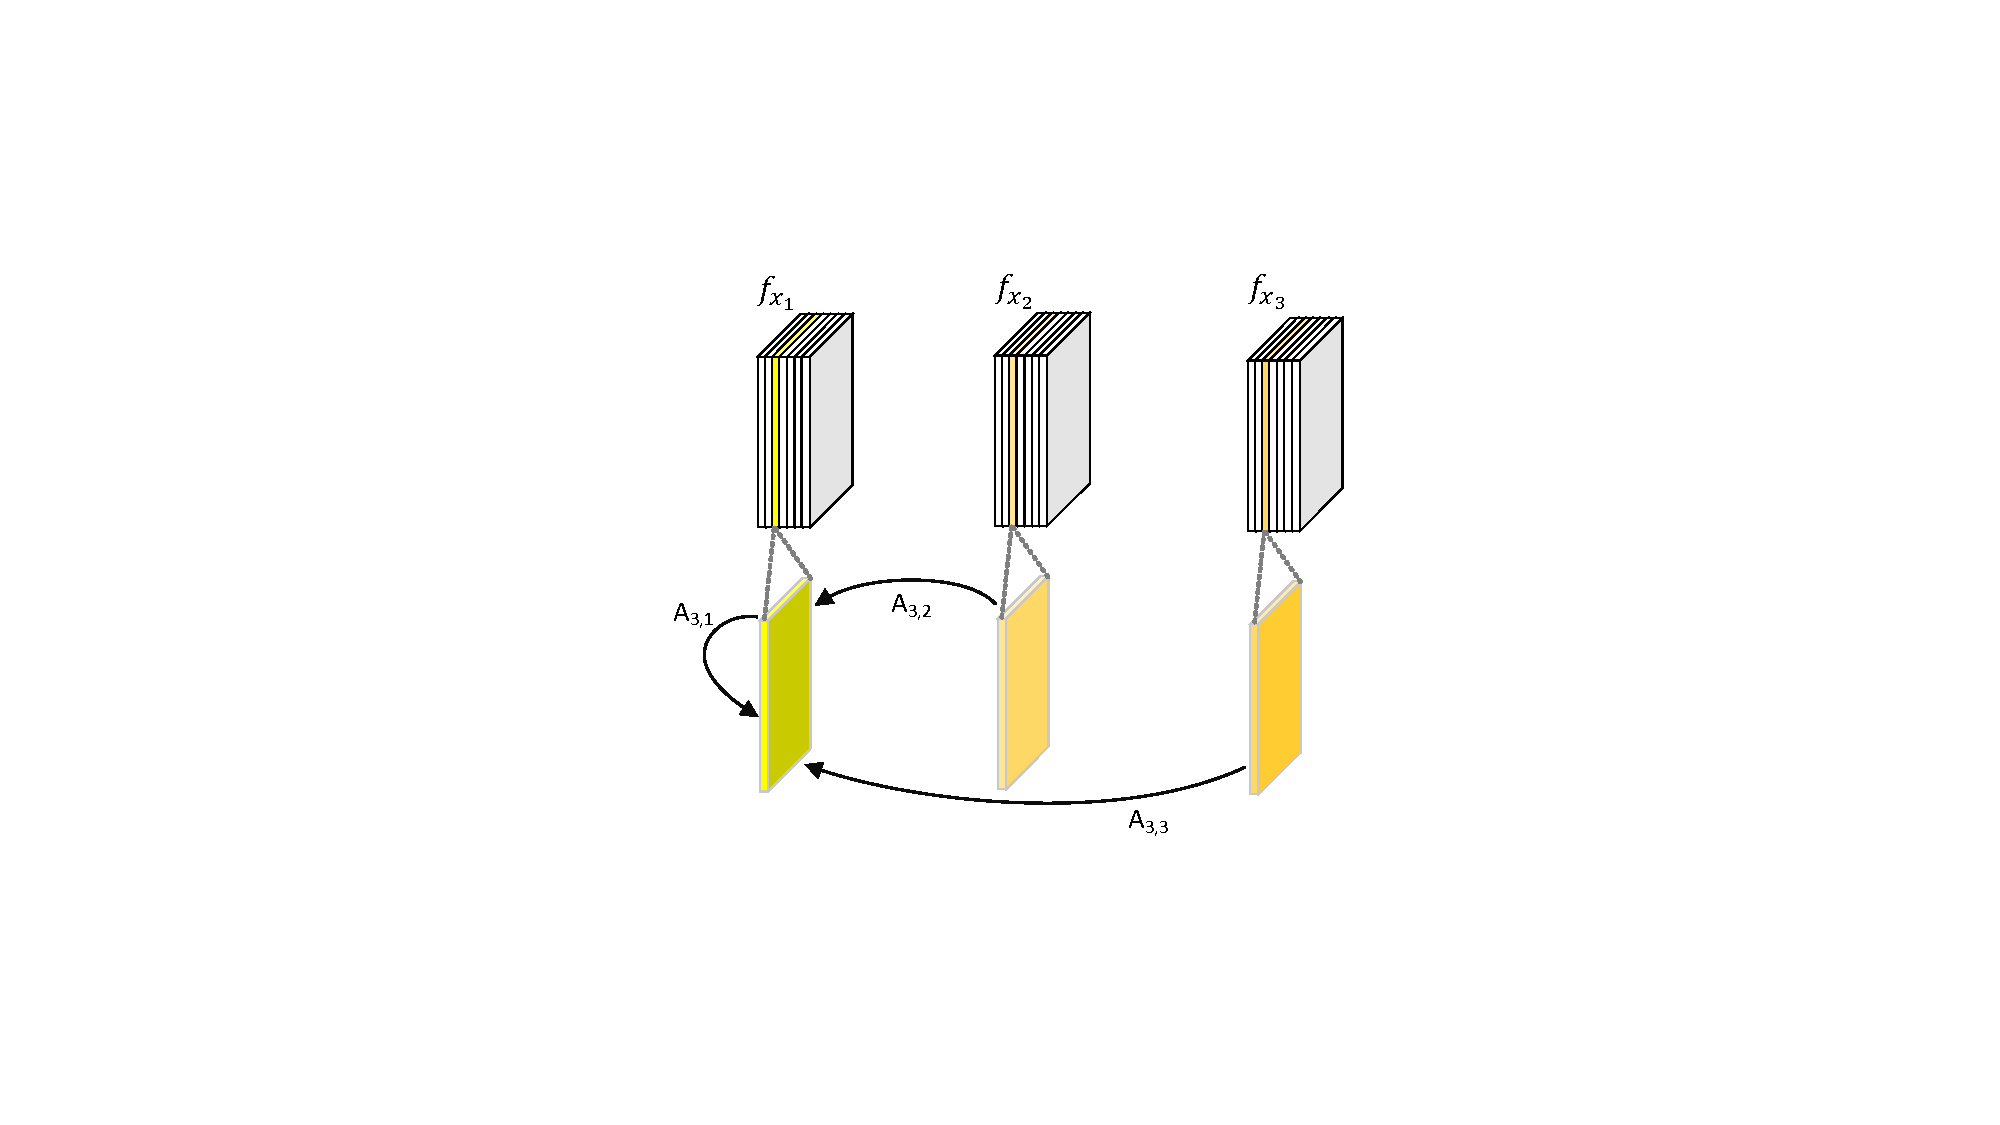
\includegraphics[width=0.8\columnwidth]{figures/JAGAN/20201109InterAttention_function_BV1_0.pdf}
	\caption[aaa]{信息互补的过程. $A_{i,j}$是$A$第$i$行第$j$的元素. 在上图中,第2种模态以权重$A_{3,2}$向第1种模态的第3个通道补充信息,第3种模态以权重$A_{3,3}$向第1种模态的第3个通道补充信息。} 
	\label{f3}
\end{figure}

\subsection{网络实现}

JAGAN由转换网络和子表示网络组成。

\textbf{网络损失} 在训练阶段,我们使用 Adam 来优化模态间注意力-GAN 的生成器 G 的总损失:
\begin{align}
	\mathcal{L}_G = \mathcal{L}_{L1} + \mathcal{L}_{GAN} + \lambda  \cdot \mathcal{L}_{intra}^{SR}
\end{align}
其中 $\mathcal{L}_{L1}$ 和 $\mathcal{L}_{GAN}$ 都是在 pix2pix 中定义的,$\lambda$ 是 $\mathcal{L}_{intra}^{SR}$ 的权重。

\textbf{转换网络} 转换网络由一个生成器和一个鉴别器组成。 我们采用70 × 70的PatchGANs\cite{pix2pix} 作为我们的鉴别器网络和来自 \cite{perceptual} 的架构用于我们的生成器。该网络包含三个用于特征提取和下采样的卷积,几个用于特征变换的残差块,以及三个用于上采样的卷积。为了适应多模态输入,我们重复构造前三个卷积 $\{Conv_1, Conv_2, Conv_3\}$ $n$ 次,形成一个多分支编码器,其中 $n$ 是输入模态的数量,$ Conv_k$ 表示第 $k$ 个卷积,每个分支以$E_i$表示。 我们将模态内注意力模块添加到 $Conv_2$ 和 $Conv_3$之间,并将模态间注意力 注意力添加到 $Conv_3$之后。为了使模型能够接收任何三种模式作为输入,我们在每个输入图像中添加目标模态的one-hot编码的mask\cite{stargan}\cite{collagan}。

\textbf{自表示网络} 自表示网络采用与生成器相同的网络结构,区别在于没有使用多分支编码器,在计算损失时没有使用 $\mathcal{L}_{GAN}$。我们将原始图像输入到自表示网络中,不添加任何mask。 实验表明,仅使用 $\mathcal{L}_{L1}$ 监督,自表示网络可以快速拟合每个数据集,并在$\mathcal{T}$的特征提取阶段提供有效的监督。


\section{实验}

\subsection{实验设置}

\subsubsection{数据集和评测标准}

\textbf{医学图像转换}
对于多模态医学图像转换任务,我们在 BraTS2020~\cite{bakas2018identifying}数据集上评测我们的方法,该数据集由四种核磁共振 (MR) 成像模式组成:T1加权成像(T1)、Gd造影剂成像(T1Gd)、T2加权成像 (T2 )和液体衰减反转恢复序列成像(T2-FLAIR)。 共有494名受试者患有低级别或高级别胶质瘤。 每个MR图像的大小为 $240\times240\times155$,体积元素大小为 $1\times 1\times 1 mm^3$ 由于这些MR图像是通过不同的临床协议和来自多个($n=19$)机构的各种扫描仪获得的,并且肿瘤实体在不同的方式下具有不同的外观,因此转换任务的难度非常大。

我们遵循BraTS2020数据集中的原始训练集测试集划分协议:369个样本作为训练集,剩下的125个样本作为测试集。

\textbf{面部图像转换}
对于多模态面部图像转换任务,我们在 Radboud Faces Database (RaFD)~\cite{langner2010presentation} 上评测我们的方法,该数据集包含八种面部表情:快乐、愤怒、悲伤、轻蔑、厌恶、中立、恐惧、惊讶;和三个注视方向:向左看、向前看、向右看。 共有67名受试者,其中男性38名,女性19名,儿童10名。

由于 RaFD 数据集的样本数量有限,我们在实验中采用了 10 折交叉验证。即90\%的数据(约 60 名受试者)构成了训练集,测试集包含剩余的 10\%(6 或 7 名受试者)数据。

\subsubsection{实现细节}
所有实验均在 PyTorch 框架下使用 NVIDIA TITAN RTX GPU 完成。我们使用动量参数 $\beta_1 = 0.5$ 和 $\beta_2 = 0.999$ 的 Adam 优化器~\cite{kingma2014adam} 优化网络参数。所有实验的批大小均设置为 1。实验过程中使用的所有图像都是空间对齐的。为了使训练更加稳定,我们先单独训练自表示网络,然后在训练转换网络时加载预先训练好的自表示网络。同时训练自表示网络和转换网络可以达到类似的准确率,但需要更多的迭代次数才能完成。

由于BraTS2020数据集中的 3D MR 图像是根据横向平面扫描的,显然它们仅在水平方向上是连续的。在这里,我们遵循扫描方向,从每个样本中提取多个切片。所有图像都缩放到 $256\times256$,并在将它们放入模型之前将像素值归一化到区间 $[-1, 1]$。超参数 $\gamma$、$\lambda$设置为 $0.5$、$0.1$、$0.1$、$3$ 和 $2$。输入和输出通道数在医学图像转换任务中为 1,在面部表情转换任务中为 3。

\subsubsection{基准方法与评测标准}

我们将我们的方法与三种最先进的基于 GAN 的图像转换方法进行比较:Pix2Pix~\cite{pix2pix}、StarGAN~\cite{stargan} 和 CollaGAN~\cite{collagan}。为了和我们的JAGAN公平比较,所有基准方法的所有结果都是在相同的数据集划分协议下训练和测试的。所有结果均来自作者提供的源代码。我们下面将从定性和定量两个角度,对我们的方法和所有基准方法进行比较。

如何评测转换图像是一个公认的难题~\cite{salimans2016improved},这是因为图像中的每个像素不是独立的,我们应该在图像维度上评测它们。因此,对于定量评测,我们采用结构相似性指标度量(SSIM)~\cite{ssim} 来评测图像级的一致性,使用特征相似性指标度量(FSIM)~\cite{fsim} 来评测特征级一致性。SSIM 和 FSIM 分数由转换后的生成图像(伪图像)及其相应的真实图像计算得出。与多模态医学图像转换任务不同,面部图像不同表情之间的运动使得很难利用 SSIM 和 FSIM 对面部图像进行定量评测。由于面部图像属于自然图像,因此,通过在ImageNet上预训练的分类模型计算得到的 Fréchet Inception Distance (FID)\cite{fid} 更适合面部图像转换任务。对于定性评测,我们将在实验部分标胶我们方法和所有基准方法的多模态图像转换结果。

\begin{figure}
	\begin{center}
		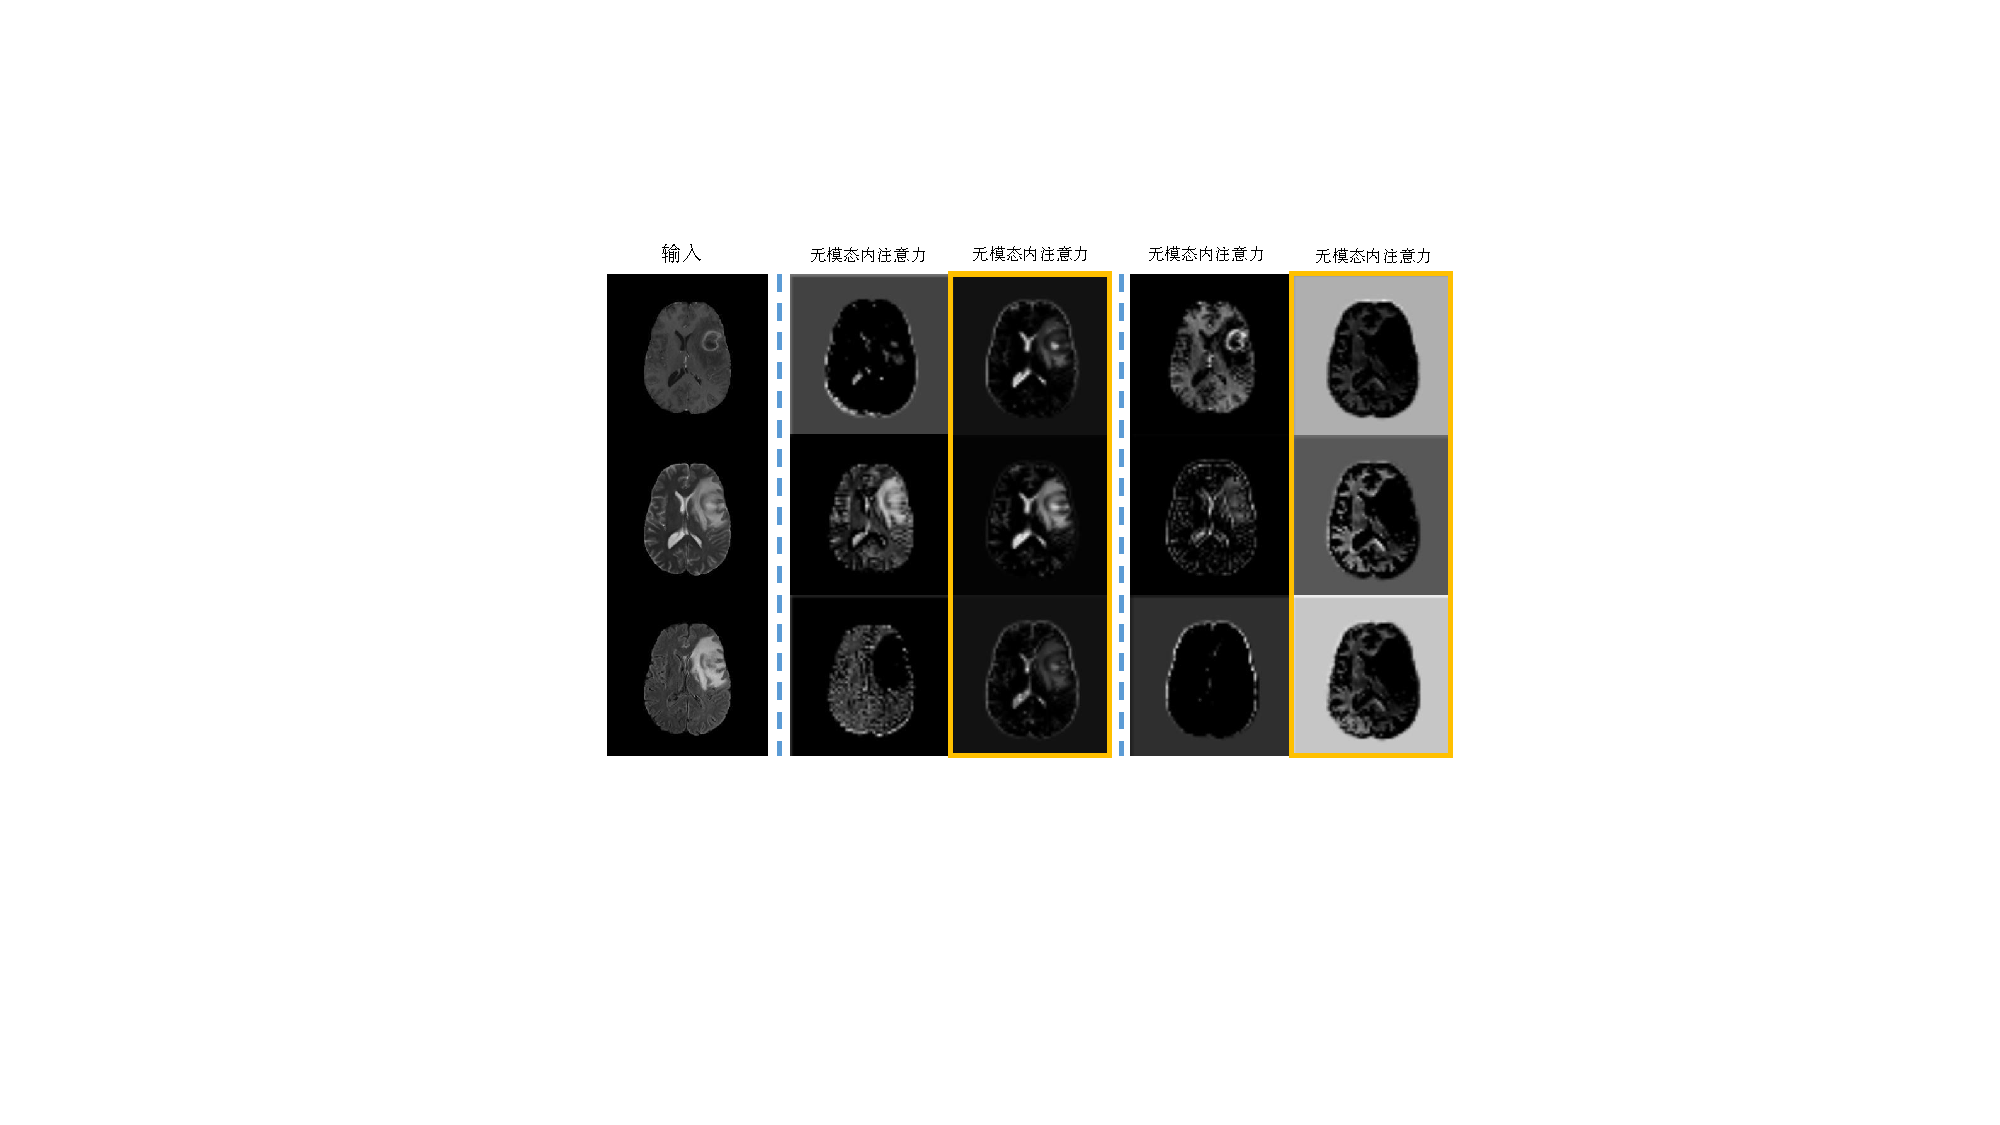
\includegraphics[width=0.8\columnwidth]{figures/JAGAN/ablation1.pdf}
	\end{center}
	\caption{特征图可视化. 同一行的特征图来源于同一个卷积核,区别在于有无自表示监督。}
	\label{fig:ablation1}
\end{figure}


\subsection{对比实验}

最近提出了各种基于 GAN 的图像转换方法。 在这些方法中,Pix2Pix~\cite{pix2pix} 是一种基于 cGAN 的方法,它是我们模型的基本架构,StarGAN~\cite{stargan} 和 CollaGAN~\cite{collagan} 提出了目标模态掩码向量和循环- 一致损失~\cite{cyclegan} 到多模态图像转换任务。因此,我们在下面的实验中将我们的方法与 Pix2Pix、StarGAN 和 CollaGAN 进行比较。

\subsubsection{MR图像转换对比}
为了评测我们所提出的方法在多模态医学图像转换上的性能,我们用Brats2020训练集中的所有数据来训练自表示网络,并从Brats2020训练集中采样三种模态的所有可能组合,作为转换网络的输入,我们可以通过这三种输入模态生成任何缺失的模态。 由于Pix2Pix和StarGAN只适合单个输入,我们选择 T2-FLAIR 作为输入,每种方法通过三个独立的 Pix2Pix 模型和一个 StarGAN 模型转换为 T1、T1Gd、T2。 因为 T2-FLAIR 可以提供肿瘤实质和水肿区域,明显大于其他三种模式。 T2-FLAIR 模态由具有独特造影剂信息的 T1Gd 模态估计。 CollaGAN 遵循与我们相同的设置。
 
 \begin{figure}
	\begin{center}
		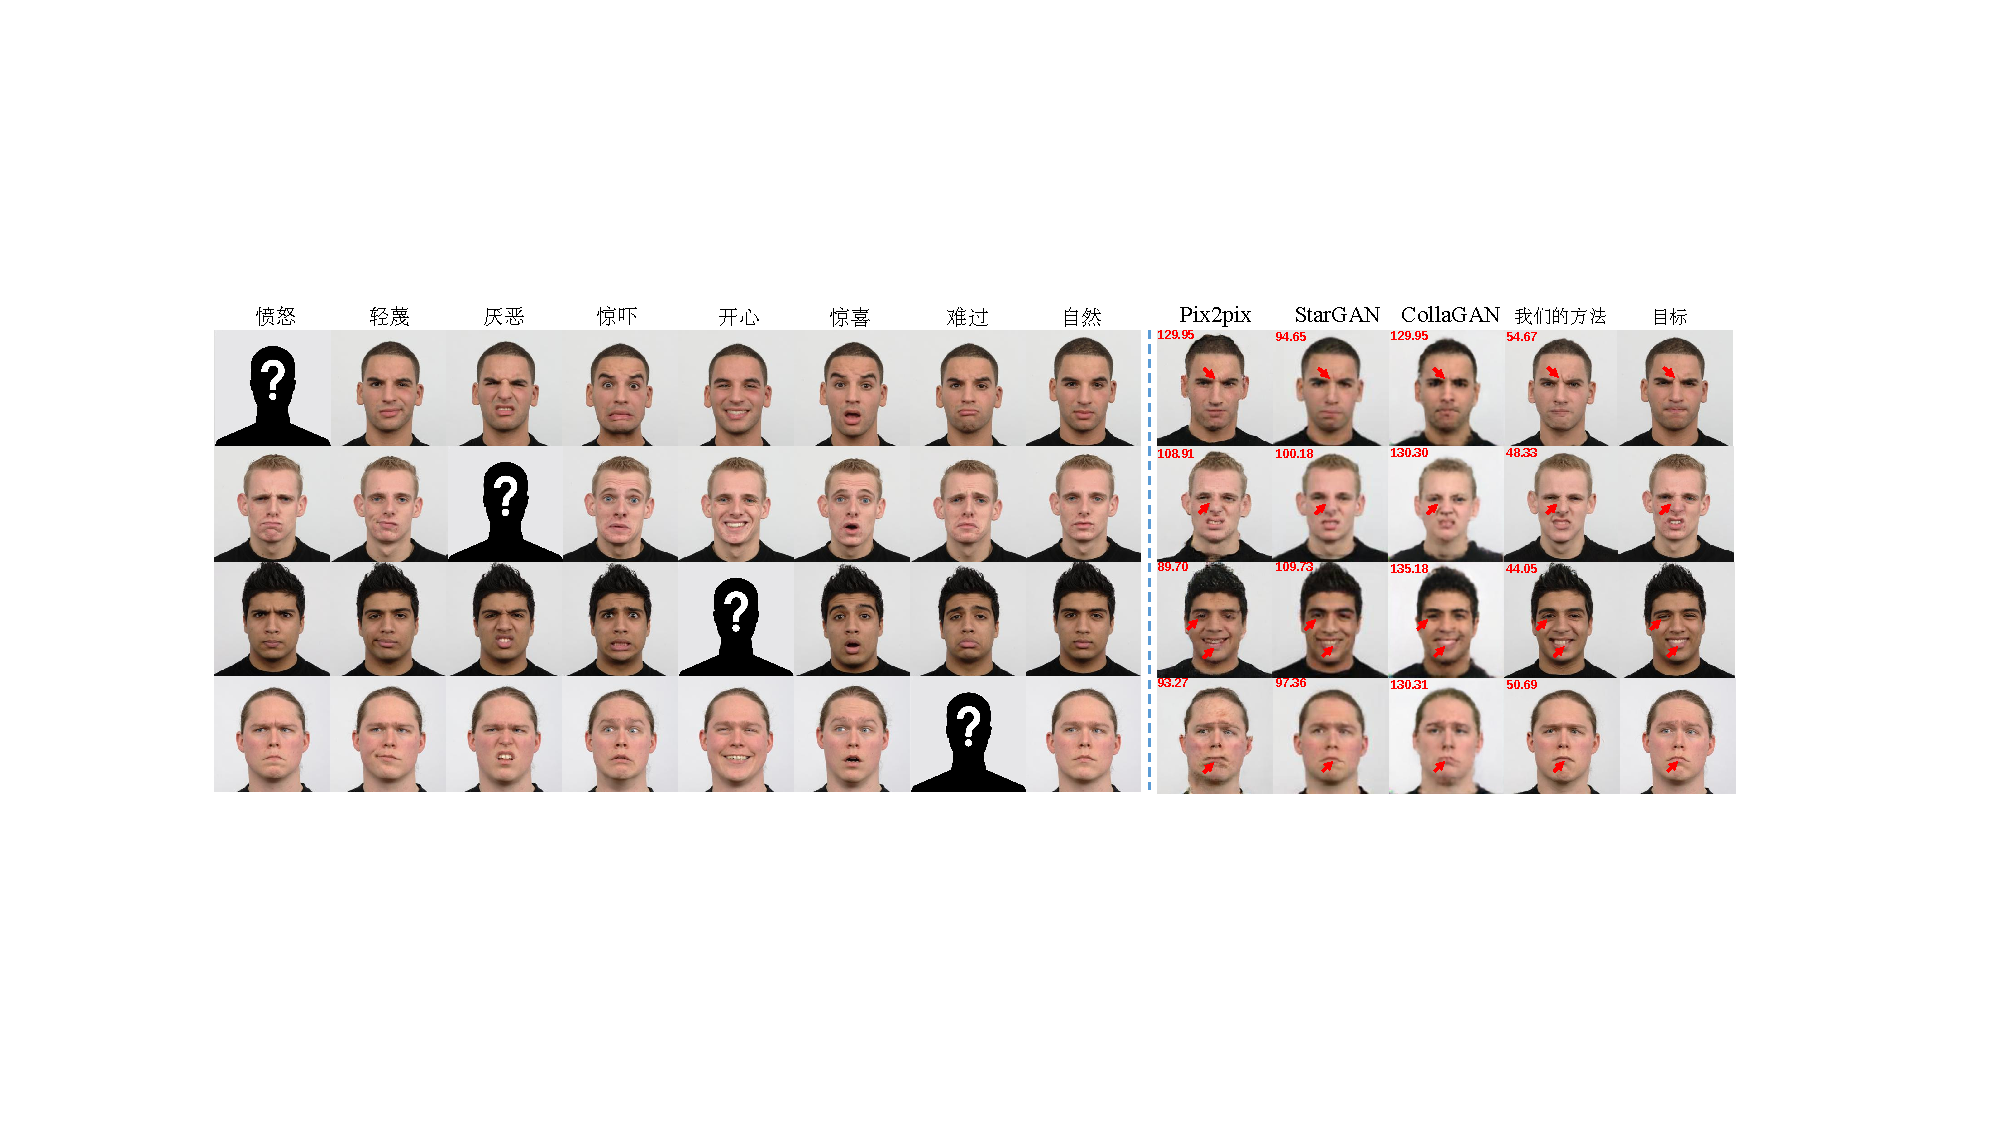
\includegraphics[width=1\columnwidth]{figures/JAGAN/comparsion_facial.pdf}
	\end{center}
	% \caption{Comparison results of our approach, Pix2Pix, StarGAN and CollaGAN on RaFD database. The red numbers are the FID scores. The arrows point out the remarkable parts of the results. For Pix2Pix and StarGAN, the pseudo images are translated from the neutral expression. Our JAGAN can generate any target modality by the remaining seven modalities.}
	\caption{我们的方法、Pix2Pix、StarGAN 和 CollaGAN 在 RaFD 数据集上的比较结果。 红色数字是 FID 分数。 箭头指出了结果的显着部分。 对于 Pix2Pix 和 StarGAN,伪图像是从中性表达转换而来的。 我们的 JAGAN 可以通过其余七种模态生成任何目标模态。}
	\label{fig:comparsion_facial}
\end{figure}

如图~\ref{fig:comparsion_medical}所示,StarGAN和CollaGAN的结果在转换T1Gd、T2和T2-FLAIR时表现出较差的感知外观。软组织细节不清晰,对比度不准确。虽然 CollaGAN 生成了可接受的肿瘤纹理,但结果嘈杂,严重降低了感知外观。 Pix2Pix 在生成 T2 和 T2-FLAIR 方面比 StarGAN 和 CollaGAN 产生更好的纹理细节,但 Pix2Pix 的结果对比不明显。与这些方法相比,我们的 JAGAN 显示出清晰的软组织纹理和明显的肿瘤病变区域。

对于定量评测,我们在每个转换样本的右下角显示了平均 SSIM 和 FSIM 分数(斜线前后)。这些报告的评测分数由转换后的图像和相应的真实图像计算得出。现有方法忽略了多模态图像中的互补信息,从而降低了定量分数。我们的 JAGAN 在完整的医学图像转换任务集上取得了最高的 SSIM 和 FSIM 分数。

请注意,由于输入限制,本实验中对 Pix2Pix 和 StarGAN 进行了多次训练。 CollaGAN 占用的计算资源比我们的多得多,但获得的结果却很模糊。作为比较,我们的 JAGAN 可以通过统一模型中的剩余数据生成任何目标医疗模式。该实验中的定量和定性比较通过显示更精确和更现实的结果证明了我们方法的优越性。

\subsubsection{面部表情转换对比}
评测所提出的多模态医学图像转换方法,我们取 RaFD 数据集训练集中的所有数据~\cite{langner2010presentation} 来训练自表示网络,并从 RaFD 数据集的训练集中选择七种模态的所有可能组合作为输入转换网络。
然后,我们可以将任何七个面部表情图像转换为剩余的目标面部表情。 Pix2Pix 和 StarGAN 的输入设置为面部表情中性,因为中性和其他样本的差异很小。 CollaGAN 适用于多个输入,因此,它与我们的共享相同的设置。

如图~\ref{fig:comparsion_facial},由于不同面部表情之间的肌肉运动,图像无法严格对齐。由于 Pix2Pix 需要配对数据,因此 Pix2Pix 在这些未对齐的面部表情图像上的转换面部图像包含很大的变形,导致感知外观较差。 StarGAN 和 CollaGAN 适用于未配对数据,因此,转换的面部表情通常是可以接受的。然而,纹理细节是模糊的,这降低了感知外观。我们提出的方法生成具有正确表情的逼真面部图像。

\begin{figure}
	\begin{center}
		\includegraphics[width=1\columnwidth]{figures/JAGAN/comparsion_medical.pdf}
	\end{center}
	% \caption{Comparison results of our approach, Pix2Pix, StarGAN and CollaGAN on BraTS2020 database. The yellow numbers are the SSIM and FSIM scores. The arrows point out the remarkable parts of the results. For Pix2Pix and StarGAN, the pseudo T1/T1Gd/T2 figures/JAGAN are translated from a T2-FLAIR image, and the T2-FLAIR image is translated from T1Gd. Our JAGAN generates any target modality by the remaining three modalities.}
	\caption{我们的方法、Pix2Pix、StarGAN 和 CollaGAN 在 BraTS2020 数据库上的比较结果。 黄色数字是 SSIM 和 FSIM 分数。 箭头指出了结果的显着部分。 对于 Pix2Pix 和 StarGAN,生成的T1/T1Gd/T2模态图像是从真实的T2-FLAIR模态图像转换而来,T2-FLAIR模态图像则是从T1Gd模态转换而来。 我们的JAGAN是通过其余三种模态生成目标模态。}
	\label{fig:comparsion_medical}
\end{figure}

对于定量评测,FID 分数显示在每个样本的左上角。分数越低意味着效果越好。 StarGAN 和 CollaGAN 的转换结果是模糊的,这导致了高 FID 分数。虽然 Pix2Pix 的结果包含更大的变形,但细节比 StarGAN 和 CollaGAN 更真实。与这些最先进的方法相比,我们的方法以最低的 FID 分数实现了最佳的定量评测。

类似于多模态医学图像转换任务,我们的方法可以通过统一模型中的其他七个面部表情生成任何面部表情。这种多模态面部表情转换实验也证明了所提出的 JAGAN 的有效性。

\subsection{消融实验}

我们对提议的框架进行了消融研究,以量化两个关键概念对整体性能的贡献。以下实验结果表明模态内注意力和模态间注意力都对改进我们的模型有效,我们由模态内注意力和模态间注意力组成的联合注意力为多模态图像转换任务产生了高质量的结果。

我们采用不同的实验设置来验证每个模块的有效性:没有模态内注意力和模态间注意力的 JAGAN、没有模态内注意力的 JAGAN 和没有模态间注意力的 JAGAN。这些方法的一些结果如图~\ref{fig:ablation}所示。基准方法方法是没有 模态内注意力 和模态间注意力的转换网络。如图~\ref{fig:ablation}(a)所示,转换后的医学图像对比度不准确,肿瘤区域估计也不准确。合成面部表情 \textit{contemptuous} 更类似于 \textit{neutral}。通过添加模态间注意力,该模型可以更好地估计医学图像的肿瘤区域,以及更准确的面部表情的嘴巴和皱纹,如图~\ref{fig:ablation}(b) 所示。这表明模态间注意力可以有效地融合模态间互补信息。然而,细节并非模糊不清。图~\ref{fig:ablation}(c)是使用模态内注意力模块的基准方法模型的结果,估计的医学图像对比度更准确,面部图像的眼睛等细节纹理更逼真。这验证了模态内注意力可以提供更多的兼容性信息。通过结合 模态内注意力 和模态间注意力,如图~\ref{fig:ablation}(d) 所示,完整的 JAGAN 模型成功地为估计的医学图像生成了最准确的对比度和肿瘤区域,以及最逼真的面部纹理表达转换。

\begin{figure}
	\begin{center}
		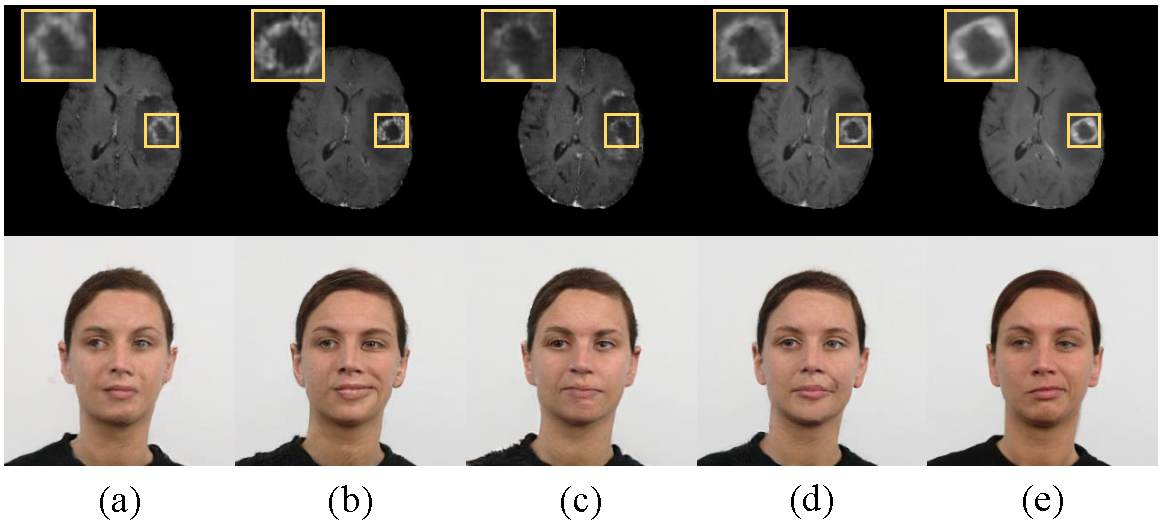
\includegraphics[width=0.8\columnwidth]{figures/JAGAN/ablation.pdf}
	\end{center}
	\caption{消融实验. (a) 没有模态内注意力和模态间注意力的JAGAN实验结果。 (b) 没有模态内注意力的JAGAN实验结果。 (c) 没有模态间注意力的JAGAN实验结果。 (d) JAGAN的实验结果。(e) 真实图像。}
	\label{fig:ablation}
\end{figure}

由于采用自表示网络来保持转换网络中间特征图的目标特定一致性。 在这里,我们探讨了自表示 (SR) 网络对不同编码器分支的卷积核的有效性。 如图~\ref{fig:ablation1}所示,在没有SR网络的情况下,由相应编码器分支从不同输入提取的特征图差异很大。 在SR网络的约束下,从同一个卷积核中提取的特征图满足具有相似外观的跨模态一致性。

为了定量评测SR网络对转换网络的约束效果,利用t-SNE~\cite{maaten2008visualizing}将提取的特征图嵌入到二维空间中,如图~\ref{fig:regression}。每种颜色代表特征图源自的编码器分支。左子图显示了从没有 SR 网络约束的某个卷积核中提取的特征图的 t-SNE 分布,右子图显示了从同一卷积中提取的特征图的 t-SNE 分布具有 SR 网络约束的内核。我们从每个编码器中选择六个卷积核。对于多模态医疗人物/JAGAN,总共有四组输入和四个编码器。因此,每个子图中有 96 个点。如图~\ref{fig:ablation1}所示,使用SR网络训练的特征图分布比没有SR网络的特征图分布更接近。特征外观和 t-SNE 分布证明了所提出的跨模态一致性的有效性。

\begin{figure}
    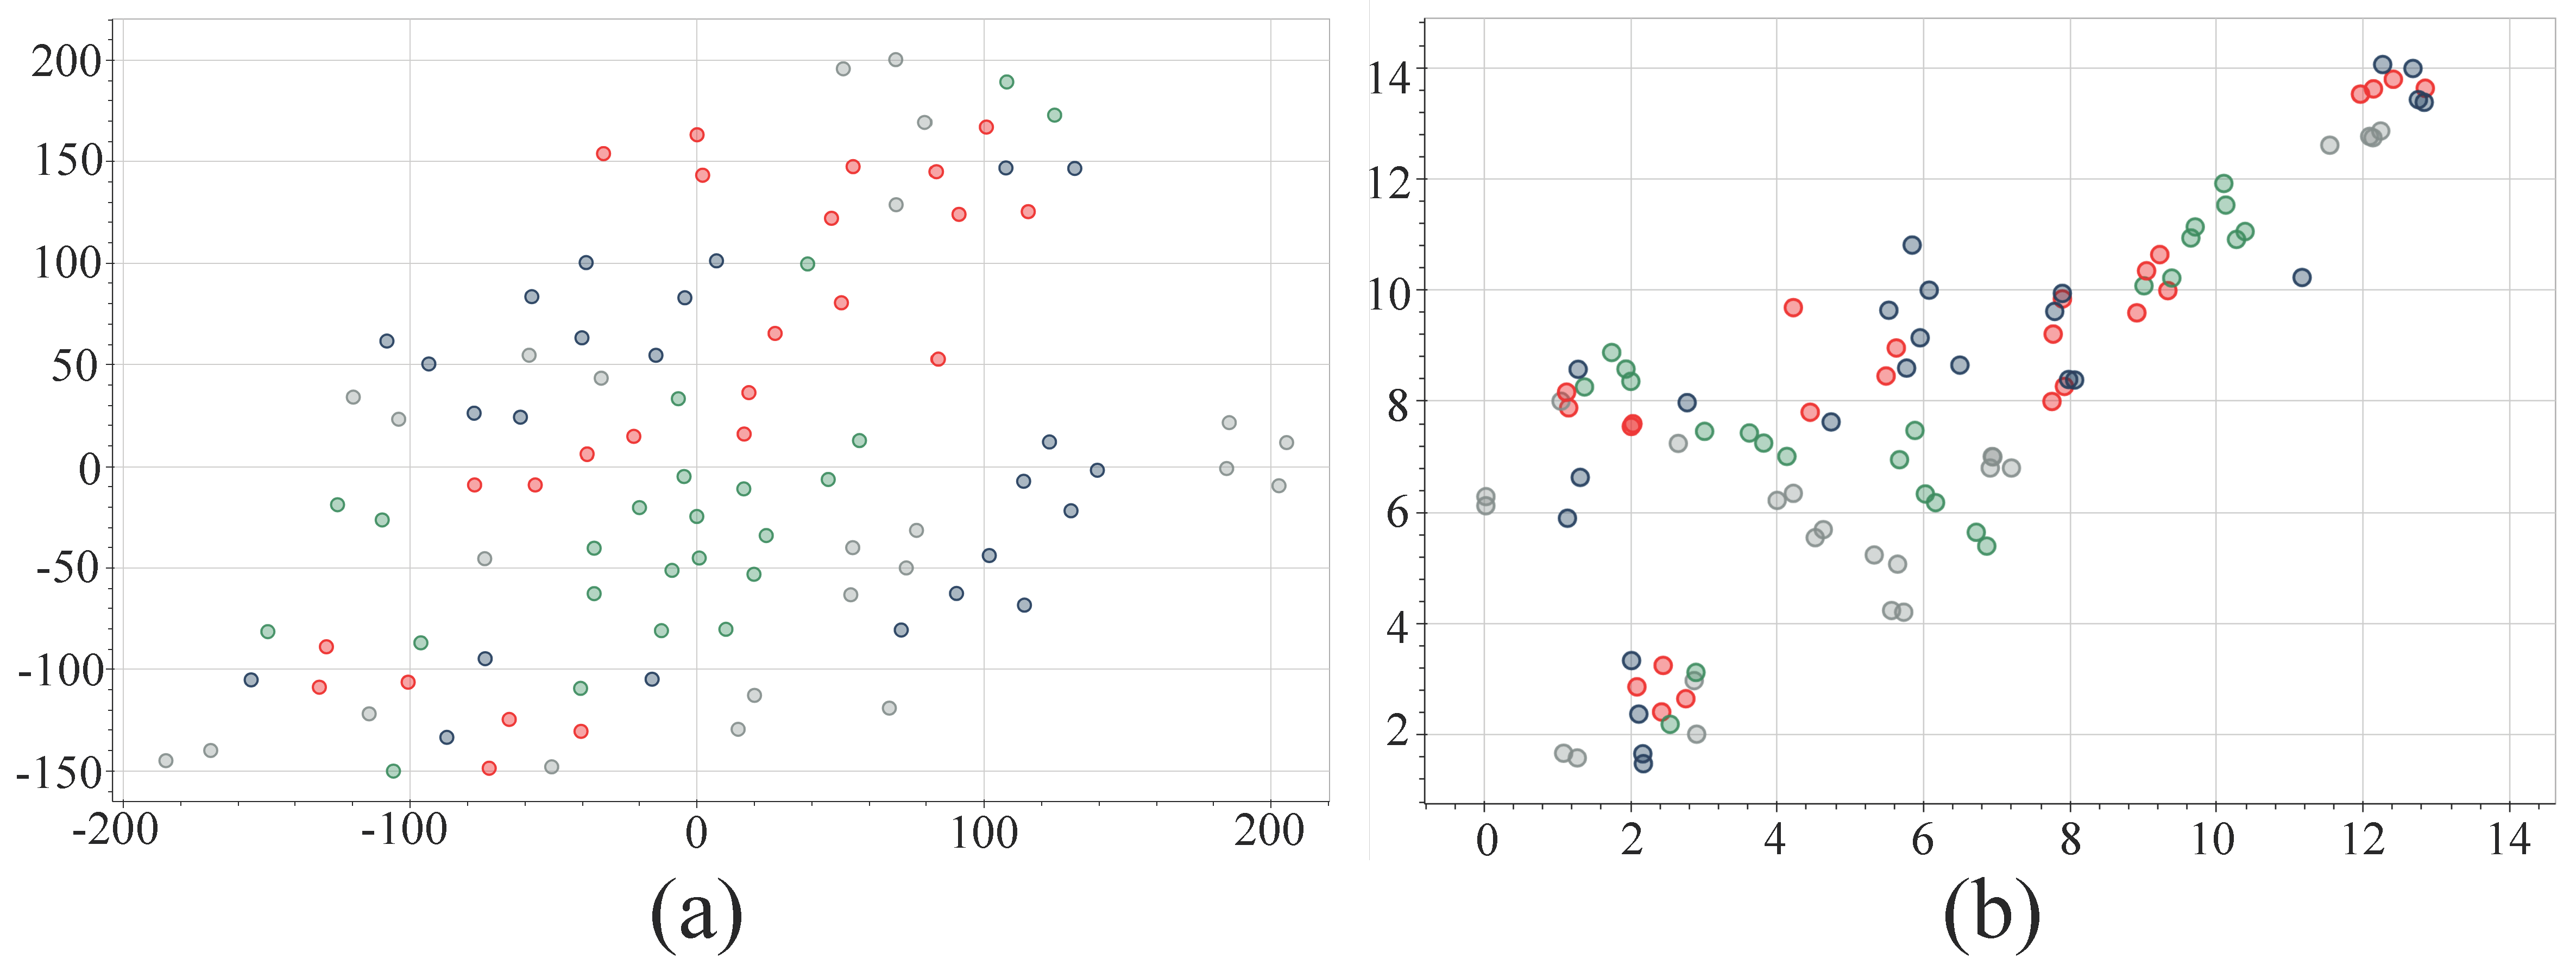
\includegraphics[width=1\columnwidth]{figures/JAGAN/regression.png}
	\caption{特征图的二维可视化。每个圆点表示一个特征图,不同的颜色表示其来源自不同的编码器分支。(a)是没有模态内注意力的结果, (b) 则是有模态内注意力的结果。}
	\label{fig:regression}
\end{figure}


\section{本章总结}

在本文中,我们提出了一种用于多模态图像转换的联合注意力 GAN。 我们的方法利用自编码器网络进行自监督学习,为多模态转换网络提供跨模态一致性指导。 我们将模态内兼容性、模态间互补性和跨模态一致性合并到一个统一的生成框架中。
自表示学习框架利用来自多种模态的多方面信息。 设计的多分支编码器和模态掩码向量使我们的 JAGAN 能够在单个统一模型中生成任何缺失的模态,进一步保证其通用性。

虽然我们提出的 JAGAN 与其他最先进的技术相比实现了卓越的性能,但存在一些局限性。例如,在训练阶段,所提出的框架需要更多的计算资源和计算时间。 未来,我们将探索更高效的网络架构。

\clearpage{\pagestyle{empty}\cleardoublepage}
\chapter{总结与展望}

\section{全文总结}

生成式对抗网络(GANs)自提出以来就一直是深度学习乃至人工智能领域的热门话题。在近几年研究人员的持续努力之下,GANs在训练稳定性、生成图像的质量方面取得了长足的进步。随着GANs生成图像真实度越来越接近真实图像,研究人员开始探索GANs的具体应用。本文梳理了GANs的发展历程和应用领域,就图像编辑和多模态图像转换展开了讨论,指出目前所存在的问题,并给出了相应的解决方案。

为了隐空间编辑语义耦合的问题,并更准确地控制生成图像的属性,本文提出了属性一致生成对抗网络(Attribute Consistent Generative Adversarial Networks),简称ACGAN。为了证明ACGAN可基于任意非条件GANs实现,本文在StyleGAN2和文献~\cite{lwgan}提出的轻量级GANs的基础上实现了ACGAN,分别用于人脸属性编辑和自然风景属性编辑。为了全面分析与展示ACGAN在属性编辑方面的优越性,本文对这两种场景下的属性编辑均设计了对应的定量与定性两类实验,其中不乏人脸属性编辑中的属性编辑成功率与保留率,和自然风景属性编辑中属性增益这样原创性的评价指标。为了将ACGAN拓展到现有的二值属性标注数据集,本文还提出了一种属性量化策略,用于生成连续的伪标签。

为了解决难以对多模态输入之间相关性建模的问题,本文提出了一种联合注意力生成式对抗网络 (Joint Attetion Generative Adversarial Networks, JAGAN),探索了如何通过注意力机制通过挖掘模态间的一致性与互补性,提出了模态内注意力和模态间注意力两种注意力机制,高效实现了利用多模态图像补全缺失的模态图像。本文在医学图像转换和面部图像转换两个场景下做了实验,展示了JAGAN相对于现有图像转换方法在多模态场景下的优越性。然后,本文通过消融实验证明了两种注意力机制的有效性,和两种注意力结合使用的必要性。

本文的贡献可归纳为以下几点:

(1)第三章提出了属性一致生成对抗网络ACGAN:GAN的隐空间被分解为内容空间和正交的语义空间,为解决隐空间编辑语义耦合问题提供了理论上的保障。本文提出属性一致性损失,引入属性回归器在训练阶段监督输入属性与生成图像属性之间的一致性。ACGAN统一了GANs生成图像与属性控制两个任务,使生成器天然具有控制生成图像属性的能力。

(2)在第三章中,为了将ACGAN应用于更常见的二值属性数据集,本文设计了一种属性量化方法,来获得连续属性伪标签。这种属性量化方法可以灵活地与现有方法集成以提高属性编辑性能。

(3)第四章提出了联合注意力生成式对抗网络JAGAN。针对多模态图像转换,提出跨模态一致性和模态间互补性的概念,指出现有方法的不足。模态内注意力依据跨模态一致性,借助自表示网络来引导生成器的训练,在特征提取阶段过滤掉无关信息,并模态信息互补提供了所需的特征兼容。模态间注意力依据模态间互补性,为每个输入模态补充生成目标模态所需要的信息。

\section{展望}

虽然我们在第三章提出的 ACGAN 与现有的隐空间编辑和图像转换方法相比实现了更加卓越的性能,但仍存在一些局限性。例如,在计算属性一致性损失时,从均匀分布采样可能会采样到矛盾的属性组合,使用图卷积神经网络(GCN)辅助采样将是非常值得尝试的方案。 此外,对真实图像的编辑十分依赖GAN逆映射(GAN inversion)的效果,这通常需要复杂的 GAN 架构,如StyleGAN2 。然而,使用StyleGAN2 实现ACGAN需要大量的训练时间。第四章提出的 JAGAN 同样存在类似的问题:JAGAN与其他最先进的技术相比实现了卓越的性能,但需要更多的计算资源和计算时间。未来,我们将探索更高效的GAN架构。

除了本文所提到的GANs在图像编辑和多模态图像转换方面的应用外,GANs实际上还有许多方面的应用,如国际计算机视觉大会(ICCV)2019最佳论文SinGAN~\cite{singan}使用单一GANs模型实现了图像相关的5种任务。除图像外,GANs还可用于语音、音乐的合成~\cite{voice1,voice2,voice3}。GANs在特定领域的应用方兴未艾,存在大量问题需要解决,值得所有GANs研究人员继续努力。
\clearpage{\pagestyle{empty}\cleardoublepage}
%%%%%%%%%% 正文部分内容  %%%%%%%%%%

%%%%%%%%%%  参考文献  %%%%%%%%%%
\defaultfont
\bibliographystyle{references/TJUThesis}
\phantomsection
\markboth{参考文献}{参考文献}
\addcontentsline{toc}{chapter}{参考文献}          % 参考文献加入到中文目录
% \nocite{*}                                       % 若将此命令屏蔽掉,则未引用的文献不会出现在文后的参考文献中。
\bibliography{references/reference}

\clearpage{\pagestyle{empty}\cleardoublepage}
% !Mode:: "TeX:UTF-8"

\markboth{发表论文和参加科研情况说明}{发表论文和参加科研情况说明}
\addcontentsline{toc}{chapter}{发表论文和参加科研情况说明}
\chapter*{发表论文和参加科研情况说明}
\setlength{\parindent}{0em}
% \textbf{(一)发表的学术论文}
% \begin{publist}
% \item XXX,XXX. Density and Non-Grid based Subspace Clustering via Kernel Density Estimation[C]. ECML-PKDD 2012, Bristol, UK.(Submitted, Under review)
% \item XXX,XXX. A tree parent storage based on hashtable for XML construction[C]. Communication Systems, Networks and Applications, Hongkong, 2010: 325-328. (EI DOI: 10.1109/ICCSNA.2010.5588732)
% \end{publist}

\vspace*{1em}
\textbf{(一)申请及已获得的专利(无专利时此项不必列出)}
\begin{publist}
\item [1]朱鹏飞, 刘家旭, 汪廉杰,等. 一种人机协同的图像目标检测数据半自动标注方法。
\end{publist}
\vspace*{1em}
% \textbf{(三)参与的科研项目}
% \begin{publist}
% \item	XXX,XXX. XX~信息管理与信息系统, ~国家自然科学基金项目.课题编号:XXXX.
% \end{publist}
\vfill
\hangafter=1\hangindent=2em\noindent

\setlength{\parindent}{2em}                   % 发表论文和参加科研情况说明
\clearpage{\pagestyle{empty}\cleardoublepage}
\markboth{致\quad 谢}{致\quad 谢}
\addcontentsline{toc}{chapter}{致\qquad 谢} %添加到目录中
\chapter*{致\qquad 谢}

在这里,我首先要感谢导师朱鹏飞副教授。朱老师是我科研道路上的引路人,在如何阅读文献、如何寻找科研灵感、如何设计实验等十分重要的科研技能方面给予了我全方位的指导。朱老师本人博学的知识,对科研事业的坚持,深深的感染了我,使我对科研产生既有严谨的态度,又有充足的热情。朱老师培养了我扎实的科研基础与严谨的科研习惯,并为了我规划了科研的方向。

然后我要感谢曹兵老师。成功的科研工作背后有无数细节上的困难,曹老师去年刚刚博士毕业,每当遇到细节上的困时,活跃在科研一线的曹老师都会与我讨论,帮我分析问题,并得出切实可行的方案。当我实验失败,情绪低落时,曹老师会以讲他本硕期间的经历、带我打羽毛球放松等方式鼓励我。总之,感谢曹兵老师这几个月以来的授业解惑。

最后我要感谢家人和同学,正是有了你们的鼓励与支持,我才能无惧困难,以积极的态度、饱满的的热情完成本文中的两个工作。我相信致谢不是别离,我希望在今后的日子里,能与各位老师、同学保持紧密的联系,共创更加美好的未来!
               % 致谢
\clearpage
\end{document}                                 % 结束全文
